%
% you should only have one "documentclass" line.  the following lines
% are samples that give various options.  the nofrontmatter option is
% nice because it suppresses the title and signature pages when you want
% to focus only on the main body of the thesis
%
% Friday April 10 2010 Ray Hylock <ray-hylock@uiowa.edu>
% documentclass options:
%   abstractpage            if you want to add an internal abstract (optional)
%   ackpage                 if you would like to add an acknowledgements page (optional)
%   algorithms              if you want a list of algorithms (optional)
%   appendix                if you have an appendix (optional)
%   copyrightpage           if you wish to copyright your thesis (optional)
%   dedicationpage          if you wish to make a dedication (optional)
%   epigraphpage            if you would like to add an epigraph to the beginning of your thesis (optional)
%   examples                if you want a list of examples (this uses the ntheorem package)
%   exampleslemmas          if you want a combined list of examples and lemmas (this uses the ntheorem package) (optional)
%   examplestheorems        if you want a combined list of examples and theorems (this uses the ntheorem package) (optional)
%   exampleslemmastheorems  if you want a combined list of examples, lemmas, and theorems (this uses the ntheorem package) (optional)
%   figures                 if you have any figures (this is required if you have even one figure)
%   lemmas                  if you want a list of lemmas (this uses the ntheorem package) (optional)
%   lemmastheorems          if you want a combined list of lemmas and theorems (this uses the ntheorem package) (optional)
%   nofrontmatter           suppresses the title and signiture pages for working on the body
%   tables                  if you have any tables (this is required if you have even one table)
%   theorems                if you want a list of theorems (this uses the ntheorem package) (optional)
%   phd                     if phd student; this will add the doctoral abstract (mandatory for PhD and DMA thesis candidates only)
%

% full options
%\documentclass[phd,abstractpage,copyrightpage,dedicationpage,epigraphpage,ackpage,figures,tables,lemmas,appendix]{uithesis}

% common options
%\documentclass[phd,dedicationpage,ackpage,figures,tables,appendix]{uithesis}

% example
\documentclass[phd,appendix,figures]{uithesis}

%=============================================================================
% User packages
%=============================================================================
\usepackage{bookmark}		% [recommended] for PDF bookmark generation
\usepackage{blindtext} 	% example text generation

%\usepackage{geometry}                % See geometry.pdf to learn the layout options. There are lots.
%\geometry{letterpaper}                   % ... or a4paper or a5paper or ... 
%\geometry{landscape}                % Activate for for rotated page geometry
%\usepackage[parfill]{parskip}    % Activate to begin paragraphs with an empty line rather than an indent
\usepackage{graphicx}
\usepackage{amsmath}
\usepackage{amssymb}
\usepackage{epstopdf}
\usepackage{hyperref}
\usepackage{float}
\usepackage{dblfloatfix}
\usepackage{tabularx}
\usepackage[nottoc,numbib]{tocbibind}
\usepackage{textcomp}
\usepackage{caption}
\DeclareGraphicsRule{.tif}{png}{.png}{`convert #1 `dirname #1`/`basename #1 .tif`.png}

\newcommand{\ra}{\ensuremath{\rightarrow}}
\newcommand{\bstt}{\symbol{92}}
\newcommand{\tildett}{\raise.17ex\hbox{$\scriptstyle\mathtt{\sim}$}}

%=============================================================================
% prelude
%=============================================================================

\title{Development And User Testing Of New User Interfaces For Mathematics And Programming Tools}
\author{Benjamin Berman}
\dept{Computer Science}

% multipleSupervisors=true for two advisors
\setboolean{multipleSupervisors}{false}
\advisor{Associate Professor Juan Pablo Hourcade}
% for multiple advisors; change <value> to line up the names
%\setboolean{multipleSupervisors}{true}
%\advisor{Advisor 1\\\hspace{<value>mm}Advisor 2...}
%
% edit the names below to have your committee members names appear
% on the signature page.  memberOne should be your advisor.
%
\memberOne{Juan Pablo Hourcade}
\memberTwo{Member Two}
\memberThree{Member Three}
\memberFour{Member Four}
\memberFive{Member Five}
\submitdate{September 2014}
\copyrightyear{2014}

\Abstract{
\blindtext
}

%\dedication{Dedication here (optional)}

%\epigraph{Epigraph here (optional)}

%\acknowledgements{Acknowledgements here (optional)}

\begin{document}

\frontmatter

%=============================================================================
\chapter{Introduction}
%=============================================================================

The general principle behind this dissertation is that in order to accomplish difficult tasks, one generally needs to make these tasks easy--for moving boulders you might want some leverage.  The significance of this principle was demonstrated to me when, a long time ago, my cello teacher pointed out that the way to play a difficult passage of music is not simply to grit one's teeth and keep practicing but to also figure out how playing those notes could, for instance, be made less physically awkward by changing the position of one's elbow.  In general, when it comes to ``virtuosic'' tasks--tasks that require large amounts of skill--it is easy to ignore this ``making things easy'' principle and focus on putting more time and effort into practicing or studying, even though following the principle is often a requirement for success.  The major goal of this dissertation is to apply the principle in the context of the virtuosic tasks that are involved in interactive theorem proving: I intend to show ways to make the difficult task of using interactive theorem provers easier by improving their user interfaces.  As well as solving serious usability problems for important and powerful tools for creating machine-checked proofs, many of the techniques I am developing and testing are widely applicable to other forms of coding.

My work has focused on the \textit{Coq} proof assistant\cite{Coq} \footnote{``Proof assistant'' and ``interactive theorem prover'' are synonymous}. In chapter~\ref{chapter:coqandtheneed}, this is justified by arguing that Coq is a particularly important and powerful, but complex and hard-to-use, interactive theorem prover.  More specifically, in chapter~\ref{chapter:coqandtheneed} I first give a description of Coq, including its significance, an example of theorem proving using the tool, a description of current user interfaces,  and some usability problems that I find particularly striking.  I continue with a description of a survey (including its results) on user interfaces for Coq that was sent to subscribers to the Coq-Club mailing list. Chapter~\ref{chapter:relatedwork} gives further motivation by summarizing related work.

The core research involved in this dissertation is described primarily in chapter~\ref{chapter:coqedit} and chapter~\ref{chapter:kcmsth}.  Chapter~\ref{chapter:coqedit} describes ``CoqEdit'', a new theorem proving environment for Coq, based on the jEdit text editor.  CoqEdit mimics the main features of existing environments for Coq, but has the important property of being relatively easy to extend using Java.  Chapter~\ref{chapter:coqedit} continues with a description of prototypes of two potential extensions to CoqEdit.  The chapter concludes with a description of a user study examining how these two extensions help, and potentially hinder, novice Coq users.

Chapter~\ref{chapter:kcmsth} describes a third prototype.  Although this prototype has not been tested with users, it presents a new, \textit{general} scheme for manipulating text that I hope may be built upon and widely applied.  The scheme involves the combination of two relatively novel ideas: ``Keyboard-Card Menus'' and ``Syntax Tree Highlighting''.  I describe both these two ideas and how they may be combined to help, for instance, introductory logic students using a particular subset of Coq.

There are several points that I hope will become clear in this dissertation.  First is how the research makes a \textit{positive} contribution to society.  While Coq is a powerful tool, and is already being used for important work, its power has come at the cost of complexity, which makes the tool difficult to learn and use.  Finding and implementing better ways of dealing with this complexity through the user interface of the tool can allow more users to perform a greater number, and a greater variety, of tasks.  At a more general level, the research contributes to a small but growing literature on user interfaces for proof assistants.\footnote{The research draws from and contributes to two generally separate sub-disciplines of computer science, namely programming languages theory and human-computer interaction.  I have Professors Juan Pablo Hourcade and Aaron Stump to thank for facilitating, and being involved with, unusual interdisciplinary work.}  The work this literature represents can be viewed as an extension of work on proof assistants, which in turn can be viewed as an extension of work on symbolic logic:  symbolic logic aims to make working with statements easier, proof assistants aim to make working with symbolic logic easier, and user interfaces for proof assistants aim to make working with proof assistants easier.  These all are part of the (positive, I hope we can assume) academic effort to improve argumentative clarity and factual certainty.  
	
In addition, generalized somewhat differently, the research contributes to our notions of how user interfaces can help people write code with a computer.  The complexities of the tool in fact help make it suitable for such research, since a) they are partly the result of the variety of features of the tool and tasks for which the tool may be used (each of which provides an opportunity for design) and b) the difficulties caused by the complexity may make the effects of good user interface design more apparent.  Furthermore, although Coq has properties that make it very appealing for developing programs (in particular, programs that are free of bugs), it also pushes at the boundaries of languages that programmers may consider practical for the time-constrained software development of the ``real world''.  However, if, as in the proposed research, we design user interfaces that address the specific problems associated with using a language, perhaps making the user interface as integral to using the language as its syntax, these boundaries may shift outward.  This means that not only are we improving the usability of languages in which people already are coding, we are also expanding the range of languages in which coding is actually possible.

The second point that I hope will become clear in this dissertation is that this research is an \textit{intellectual} contribution, i.e. that the project requires some hard original thinking.  User interface development is sometimes ``just'' a matter of selecting some buttons and other widgets, laying them out in a window, and connecting them to code from the back end.  While this sort of work can actually be somewhat challenging to do right (just one of the hurdles is that testing is difficult to automate), the project goes well beyond this by identifying specific problems, inventing novel solutions, and testing these solutions with human subjects.

The third and final point to be made clear in this dissertation is simply that developing and testing new user interfaces for mathematics and programming tools is a rich area of research.  Further important and interesting questions can be both raised and answered.


%=============================================================================
\chapter{Coq and the Need for Improved User Interfaces}
\label{chapter:coqandtheneed}
%=============================================================================

%%================================
\section{Basic Theorem Proving in Coq}
\label{examplesection}
%%================================

Basic theorem proving in Coq can be thought of as the process of creating a ``proof tree'' of inferences.  The user first enters the lemma (or theorem) he or she wishes to prove.  The system responds by printing out the lemma again, generally in essentially the same form; this response is the root ``goal'' of the tree.  The user then enters a ``tactic''--a short command like ``apply more\_general\_lemma''--into the system, and the system will respond by producing either an error message (to indicate that the tactic may not be applied to the goal) or by replacing the goal with zero or more new child goals, one of which will be ``in focus'' as the ``current'' goal.  Proving all of these new child goals will prove the parent goal (if zero new child goals were produced, the goal is proved immediately).  Proving the current goal may be done using the same technique used with its parent, i.e. entering a tactic to replace the goal with a (possibly empty) set of child goals to prove, and which goal is the current goal changes automatically as goals are introduced and eliminated.  The original lemma is proved if tactics have successfully been used to create a finite tree of descendants, i.e. when there are no more goals to prove.

One example useful in making this more clear can be found in Huet, Kahn, and Paulin-Mohring's Coq tutorial \cite{huet1997coq}. Assume, for now, that we are just using Coq's read-eval-print loop, ``\texttt{coqtop}''.  Consider the lemma
\begin{equation}\label{exampleLemma}(A \ra B \ra C) \ra (A \ra B) \ra A \ra C\end{equation}
where $A$, $B$, and $C$ are propositional variables and ``\ra'' means ``implies'' and is right-associative\footnote{So this lemma is equivalent to $(A \ra (B \ra C)) \ra ((A \ra B) \ra (A \ra C))$} (I discuss later how improved user interfaces may assist users, particularly novice users, in dealing with operator associativities and precedences).  Assuming, also, that we have opened up a new ``section'' where we have told Coq that $A$, $B$, and $C$ are propositional variables, when we enter this lemma at the prompt, Coq responds by printing out
\begin{quote}
\texttt{ \\
%1 subgoals \\
A : Prop \\
B : Prop \\
C : Prop \\
\_\_\_\_\_\_\_\_\_\_\_\_\_\_\_\_\_\_\_\_\_\_\_\_\_\_\_\_\_\_\_\_\_\_\_\_\_\_ \\%(1/1) \\
(A -> B -> C) -> (A -> B) -> A -> C \\}

\end{quote}


% Consider a lemma, call it \texttt{SimpleLemma} that states
%\begin{quote}
%\texttt{(A -> B -> C) -> (A -> B) -> A -> C}
%\end{quote}
%where \texttt{A}, \texttt{B}, and \texttt{C} are propositions (abbreviated in Coq as ``\texttt{Prop}''), and \texttt{->} is interpreted as ``implies'' and is right %associative (so the lemma may equivalently be written 
%\begin{quote}
%\texttt{(A -> (B -> C)) -> ((A -> B) -> (A -> C))}
%\end{quote}
%I discuss later how improved user interfaces may assist users, particularly novice users, in dealing with operator associativities and precedences).  Coq users generally think of this lemma as the sequent
For the purposes of this example, I will write such ``sequents'' using the standard turnstile ($\vdash$) notation.  The response then becomes: 
\begin{equation}\label{initialGoal}A : Prop, B : Prop, C : Prop \vdash (A \ra B \ra C) \ra (A \ra B) \ra A \ra C\end{equation}
%\[A : Prop, B : Prop, C : Prop \vdash (A \ra B \ra C) \ra (A \ra B) \ra A \ra C\]

In general, the statements to the left of the $\vdash$, separated by commas, give the ``context'' in which the provability of the statement to the right of the turnstile is to be considered.\footnote{Another list of statements, Coq's ``environment,'' is implicitly to the left of the turnstile.  The distinction between environment and context is that statements in the context are considered true only locally, i.e. only for either the current section of lemmas being proved or for the particular goal being proved.  Generally, the environment is large, and contains many irrelevant statements, so displaying it is not considered worth the trouble.}  Another way to think about the sequent is that the statements to the left of the turnstile, taken together, entail the statement to the right (or, at least, that is what we would like to prove).  In this example sequent's context, the colon indicates type, so for instance ``$A : Prop$'' just means ``$A$ is a variable of type $Prop$'' or, equivalently, ``$A$ is a proposition.''

Note that this is an extremely simple example; one could actually use Coq's \texttt{auto} tactic to prove it automatically.  Theorems and lemmas in Coq typically involve many types and operators besides propositions and implications.  Other standard introductory examples involve natural numbers and lists, along with their associated operators and the other usual operators for propositions (e.g. negation).  In fact, Coq's \textit{Gallina} language allows users to declare or define variables, functions, types, constructors for types, axioms, etc., allowing users to model and reason about, for instance, the possible effects of statements in a programming language, or more general mathematics like points and lines in geometry.

The sequence of tactics, ``\texttt{intro H}'', ``\texttt{intros H' HA}'', ``\texttt{apply H}'', ``\texttt{exact HA}'', ``\texttt{apply H'}'', and finally ``\texttt{exact HA}'' can be used to prove the sequent above (\texttt{H}, \texttt{H'}, and \texttt{HA} are arguments given to \texttt{intro}, \texttt{intros}, \texttt{apply}, and \texttt{exact}).  The first tactic, ``\texttt{intro H}'', operates on \eqref{initialGoal}, moving the left side of the outermost implication (to the right of the turnstile) into the context (i.e. the left side of the turnstile).  The new subgoal, replacing \eqref{initialGoal}, therefore is
\begin{equation}\label{introHResult}A : Prop, B : Prop, C : Prop, H : A \ra B \ra C \vdash (A \ra B) \ra A \ra C\end{equation}
%\[A : Prop, B : Prop, C : Prop, H : A \ra B \ra C \vdash (A \ra B) \ra A \ra C\]
The colon in the statement ``$H : A \ra B \ra C$'' is generally interpreted differently, by the user, than the colons in ``$A : Prop, B : Prop, C : Prop$''.  Instead of stating that ``$H$ \textit{is of type} $A \ra B \ra C$'', the user should likely interpret the statement as ``$H$ \textit{is proof of} $A \ra B \ra C$''.  However, for theoretical reasons, namely the Curry-Howard correspondence between proofs and the formulas they prove, on the one hand, and terms\footnote{``Terms,'' such as the ``$A$'' in ``$A : Prop$'', are roughly the same as terminating programs or subcomponents thereof; they may be evaluated to some final value.  Note also that, in Coq, the types of terms are terms themselves and have their own types (not all terms are types, however).  A type of the form $\it{\Phi} \ra \it{\Theta}$, where both $\it{\Phi}$ and $\it{\Theta}$ are types that may or may not also contain \ra~symbols, is the type of a function term from terms of type $\it{\Phi}$ to terms of type $\it{\Theta}$.  For instance, a term of type $nat \ra nat$ would be a function from natural numbers to natural numbers.} and types they inhabit, on the other, Coq is allowed to ignore this distinction and interpret the colon uniformly.  If fact, in proving a theorem, a Coq user actually constructs a program with a type corresponding to the theorem.  This apparent overloading of the colon operator may be a source of confusion for novice users and while there are no implemented plans in this dissertation for directly mitigating the confusion, extensions to the described user interfaces might do so by marking which colons should be interpreted in which ways.  Furthermore, by clarifying other aspects of the system, I hope to free up more of novice users' time and energy for understanding this and other important aspects of theorem proving with Coq that may not be addressable through user interface work. 

Tactics allow users to reason ``backwards''--if the user proves the new sequents(s), then the user has proved the old sequent.  In other words, the user is trying to figure out what could explain the current goal, instead of trying to figure out what the current goal entails.\footnote{Another possible point of confusion for novice users:  when the differences between the old and new sequents are in the contexts, rather than the succedents (i.e. on the left of the turnstiles rather than on the right) we may say we are doing forward reasoning, even though we are still adding new goals further away from our root goal.  This may make most sense when one views a sequent as a partially completed Fitch-style proof---this forward reasoning is at the level of statements within sequents, rather than at the level of sequents.}  Above, the (successful) use of the ``\texttt{intro}'' tactic allows the user to state that {\bf if} given a context containing that $A$, $B$, and $C$ are propositions \textit{and} $A \ra B \ra C$ it is necessarily the case that $(A \ra B) \ra A \ra C$, {\bf then} given a context containing only that $A$, $B$, and $C$ are propositions it is the case that $(A \ra B \ra C) \ra (A \ra B) \ra A \ra C$.  The fact that the tactic produced no error allows the user to be much more certain about the truth of this statement than he would if he just checked it by hand.\footnote{In general some uncertainty remains when using computer programs to check proofs. One danger is the possibility of mistranslating back and forth between the user's natural language and the computer program's language--this might happen, for instance, if a novice user were to assume an operator is left-associative when it is actually right-associative.  Another related danger, perhaps even more serious, is the possibility of stating the wrong theorem, or set of theorems.  For instance, a user might prove that some function, $f$, never returns zero, but that user might then forget to prove that some other function, $g$, also never returns zero.  An important role of theorem prover user interfaces is to mitigate these dangers by providing clear feedback and by making additional checks easier (e.g. quickly checking that $f(-1) = 1$, $f(0) = 1$, and $f(1) = 3$ might help the user realize that the property of $f$ that he actually wants to prove is that its return value is positive, not just nonzero).}

%proving that various functions defined in terms of $f$ and $g$ have the properties we expect them to have gives us additional confidence that $f$ and $g$ are acceptably defined).

%the possibility of misstating the theorem to be proved, for instance, is a serious danger

The tactic ``\texttt{intros H' HA}'' is equivalent to two intro tactics, ``\texttt{intro H'}'' followed by ``\texttt{intro HA}'', so it replaces \eqref{introHResult} with
\begin{equation}\label{introsResult}A : Prop, B : Prop, C : Prop, H : A \ra B \ra C, H' : A \ra B,  HA : A \vdash C\end{equation}
%\[A : Prop, B : Prop, C : Prop, H : A \ra B \ra C, H' : A \ra B,  HA : A \vdash C\]

Next, the tactic ``\texttt{apply H}'' replaces \eqref{introsResult} with \textit{two} new subgoals:
\begin{equation}\label{applyHresult1}A : Prop, B : Prop, C : Prop, H : A \ra B \ra C, H' : A \ra B,  HA : A \vdash A\end{equation}
%\[A : Prop, B : Prop, C : Prop, H : A \ra B \ra C, H' : A \ra B,  HA : A \vdash A\]
and
\begin{equation}\label{applyHresult2}A : Prop, B : Prop, C : Prop, H : A \ra B \ra C, H' : A \ra B,  HA : A \vdash B\end{equation}
%\[A : Prop, B : Prop, C : Prop, H : A \ra B \ra C, H' : A \ra B,  HA : A \vdash B\]
This successful use of ``\texttt{apply H}'' says that the proof $H$, that $A \ra (B \ra C)$, (parentheses added just for clarity) can be used to prove $C$, but, in order to do so, the user must prove both $A$ and $B$.  Note that, in contrast with use of the \texttt{intro} tactic, after using the \texttt{apply} tactic the contexts in the child goals are the same as in the parent.  Also note that the first of these two becomes the current goal.

The next tactic, ``\texttt{exact HA},'' eliminates \eqref{applyHresult1} without replacing it with any new goal (which makes sense, since if there is already proof of \texttt{A}, in this case \texttt{HA} in the context, then there is nothing left to do;  ``\texttt{apply HA}'' would have the same effect), and focus moves automatically to \eqref{applyHresult2}.  The tactic ``\texttt{apply H'}'' replaces \eqref{applyHresult2} with a new goal, but this new goal is identical to \eqref{applyHresult1} (we can use $A \ra B$ to prove $B$ if we can prove $A$), and so ``\texttt{exact HA}'' can be used again to to eliminate it.  Since there are no more goals, the proof is complete.

%%================================
\section{Coq's Significance}
%%================================

The example above is intended to give some sense of what interactive theorem proving with Coq is all about, and the complexities that novice users face, but it barely scratches the surface of Coq's full power and complexity.  It also does little to suggest Coq's significance.    Most of the applications accounting for this importance can be divided into those relating (more directly) to computer science and those relating to mathematics.\footnote{See the categorization of user contributions on the Coq website:  http://coq.inria.fr/pylons/pylons/contribs/bycat/v8.4}

On the computer science side, Coq has an important place in research on ensuring that computer software and hardware is free of bugs.  Given the increasing use of computers in areas where bugs (including security vulnerabilities) can have serious negative consequences (aviation, banking, heath care, etc.), such research is becoming increasingly important.  Given, also, that exhaustive testing of the systems involved in these areas is generally infeasible, researchers have recognized the need to actually prove the correctness of these systems (i.e. that the systems conform to their specifications and that the specifications themselves have reasonable properties). While fully-automatic SAT solvers (for propositional satisfiability) and SMT (satisfiability modulo theory) solvers are being used to implement advanced static analysis techniques with promising results (e.g. \cite{gulwani2008program,dillig2011small}) and can determine the satisfiability of large numbers of large formulas, keeping humans involved in the theorem proving process allows the search for a proof to be tailored to the particular theorem at hand, and therefore allows a wider range, in a sense, of theorems to be proved.  Furthermore, contrary to what might have been suggested by the step-by-step detail of the example above, many subproblems can be solved automatically by Coq and other interactive theorem provers, and work is being done to send subproblems of interactive theorem provers to automatic tools \cite{bohme2010sledgehammer} in order to combine the best of both worlds.  Notable computer science-related achievements, some in industrial contexts, for Coq and other interactive theorem provers include verification of the seL4 microkernel \cite{klein2010sel4} in Isabelle\cite{Isabelle}, the CompCert verified compiler\cite{leroy2009formal} for Clight (a large subset of the C programming language) in Coq, Java Card EAL7 certification\cite{gemaltogemalto} using Coq, and, at higher levels of abstraction, verification of the type safety of a semantics for Standard ML \cite{lee2007towards} using Twelf\cite{Twelf} and use of the CertiCrypt framework \cite{CertiCrypt} built on top of of Coq to verify cryptographic protocols (e.g. \cite{barthe2010machine}).\footnote{An earlier version of this paragraph, from which come most of the included references, was written by Dr. Aaron Stump for an unpublished research proposal.  Many of the references from the next paragraph also come from this proposal.}

On the mathematics side, Coq is being used to formalize and check proofs of a variety of mathematical sub-disciplines, as demonstrated by user contributions listed on the Coq website.  Perhaps Coq's most notable success story is its use in proving the Four Color Theorem \cite{gonthier2005computer}.  Other interactive theorem provers are also having success in general mathematics.  For instance, Matita \cite{Matita}, which is closely related to Coq, was used in a proof of Lebesgue's dominated convergence theorem \cite{coen2008constructive}.  There are in fact efforts to create libraries of formalized, machine-checked mathematics, the largest of which is the Mizar Mathematical Library \cite{geuvers2009proof}.  ITPs are also a potential competitor for computer algebra systems (e.g. Mathematica) with the major advantage that they allow transparency in the reasoning process, a significant factor limiting computer algebra use in mathematics research according to \cite{bunt2009friend}.

The potential for transparency also helps make interactive theorem provers, like Coq, a potentially useful tool in mathematics, logic, and computer science education.  Rather than simply giving students the answers to homework problems, interactive theorem provers might be used to to check students' work, find the precise location of errors and correct misconceptions early.  Interest in adapting theorem provers for educational purposes can be seen in many references listed later in this document; Benjamin Pierce et al.'s \textit{Software Foundations}\cite{pierce2010software}, a textbook, written mostly as comments in files containing Coq code and which includes exercises having solutions that may be checked by Coq, serves as an example of how the tool can be effectively used in education.  More general interest in educational systems that check student work can be seen in logic tutorial systems such as \textit{P-Logic Tutor} \cite{lukins2002tutorial}, \textit{Logic Tutor} \cite{lesta2002intelligent}, \textit{Fitch} (software accompanying the textbook \textit{Language, Proof, and Logic} \cite{barwise2000language}), and \textit{ProofMood}\cite{ProofMood}.

The part of the case for Coq's significance that is presented above is more a case for interactive theorem provers in general than Coq in particular; after reading it one may wonder, why try to improve Coq usability instead of usability for some other proof assistant?  The answer is that it is already one of the most powerful and successful such tools.  Adam Chlipala, in the introduction to his book \textit{Certified Programming with Dependent Types} \cite{chlipala2011certified}, presents a list of major advantages over other proof assistants in use:  its use of a higher-order language with dependent types, the fact that it produces proofs that can be checked by a small program (i.e. it satisfies the ``de Bruijn criterion''), its proof automation language, and its support for ``proof by reflection.''
\footnote{Basically, this is proof by providing a procedure to get a proof.  Coq allows one to prove that these procedures produce correct proofs.}  As further evidence of its resulting success, note that Coq was awarded both the 2013 ACM SIGPLAN Programming Languages Software Award \cite{CoqSIGPLANAward} and the 2013 ACM Software System Award \cite{CoqACMSoftwareSystemAward}.

%%================================
\section{Current User Interfaces and Problems They Present to Novice Users}
\label{currentUIproblems}
%%================================

The example presented earlier can be used to illustrate some more of the common challenges for users.  For novice users, one of the biggest challenges is to discover exactly what Coq's tactics do when applied to various arguments and goals.   Only four tactics were used in the example, but many more are standard (the Coq Reference Manual\cite{Coq:manual} lists almost 200 in its tactics index), and Coq allows new tactics to be defined.  Other challenges, for both novice and expert users, will be discussed below, but the lack of support for users trying to understand tactic effects is, by itself, probably sufficient justification for the development of new user interfaces.

The two major user interfaces for Coq are currently \textit{Proof General}\cite{ProofGeneral,aspinall2000proof} and \textit{CoqIDE} (which is available from the Coq website\cite{Coq}, and is bundled with Coq).  Interacting with Coq using one of these interfaces is quite similar to interacting with Coq using the other, the main difference being that Proof General is actually an Emacs mode (and so has the advantages and disadvantages of the peculiarities of the Emacs text editor, e.g. numerous shortcuts and arguably a steep learning curve).

\autoref{fig:simple1_1} and \autoref{fig:simple1_2} show the CoqIde user interface as it appears while entering the proof from the the earlier example (that $(A \ra B \ra C) \ra (A \ra B) \ra A \ra C$ ) into Coq.\footnote{Note that ``\texttt{simple1}'', in ``\texttt{Lemma simple1 : (A -> B -> C) -> (A -> B) -> A -> C.}'', is the identifier we are binding to the \textit{proof} of the lemma, and not to the lemma itself.  Without recognizing this, the fact that the keyword ``\texttt{Lemma}'' could have been replaced by the keyword ``\texttt{Definition}'' may be yet another source of confusion since it suggests that Coq thinks lemmas and definitions are basically the same thing!  As one might expect, we could also bind an identifier to the lemma itself.  If we were to bind the identifier ``\texttt{SimpleLemma}'' to this lemma, we would most likely use the \texttt{Definition} keyword in combination with ``\texttt{:=}'', and write \\``\texttt{Definition (SimpleLemma : Prop) := (A -> B -> C) -> (A -> B) -> A -> C.}''}  
The larger panel, on the left, shows a script that will in general contain definitions, theorems, and the sequences of tactics used to create proofs of these theorems.\footnote{Here the declaration of A, B, and C, and the definition of the proof of the lemma are within a section that has been named ``\texttt{SimpleExamples}.''  This sets the scope A, B, and C to just the section.  Outside of the section, reference to simple1 is allowed.  However, simple1 is changed to a proof that $\forall (A : Prop), (\forall (B : Prop), (\forall (C : Prop), ((A \ra B \ra C) \ra (A \ra B) \ra A \ra C)))$, generally written \texttt{forall A B C : Prop, (A -> B -> C) -> (A -> B) -> A -> C}.}
A portion of this script, starting at the beginning, may be highlighted in green to show that it has been successfully processed by Coq. Another portion of the script, following this green highlighting or starting at the beginning if there is no green highlighting, may be highlighted in blue to show where the ``sentences'' of the script are either being evaluated or have been queued for evaluation (sentences in the script are separated by periods followed by whitespace, as in English).  Whenever Coq is not already processing a sentence, and there are queued sentences, the first sentence in the queue is automatically dequeued and sent to Coq, so if there is a first blue-highlighted sentence, Coq is trying to evaluate it.



If a sentence is successfully processed, its highlighting changes to green and the output resulting from the successful processing is printed in one of the two panels on the right side of the window.  Assuming the system is in ``proof mode'' (e.g. after processing the sentence ``\texttt{Lemma simple1}...'' in \autoref{fig:simple1_1} and \autoref{fig:simple1_2}, but before evaluating ``\texttt{Qed.}''), the top panel displays the current goal, including its context, followed by just the consequents of any remaining goals.  The bottom panel is used to display various messages, e.g. error messages and acknowledgements of successful definitions. Otherwise, if processing of a sentence results in an error, all sentences queued for processing are removed from the queue, the blue highlighting representing that queue is removed, and the font of the offending part of the offending sentence is changed to bold, underlined red.  In general, processing a sentence is not guaranteed to produce a result of any kind (error or otherwise) in any specified amount of time (some sentences are semi-decision procedures), so CoqIde allows users to interrupt the processing of a sentence.  This also has the effect of removing all sentences from the processing queue and removing all blue highlighting. Frequently, however, processing is fast enough that the blue highlighting is never actually visible to the user.

\begin{figure}[H]
  \center
  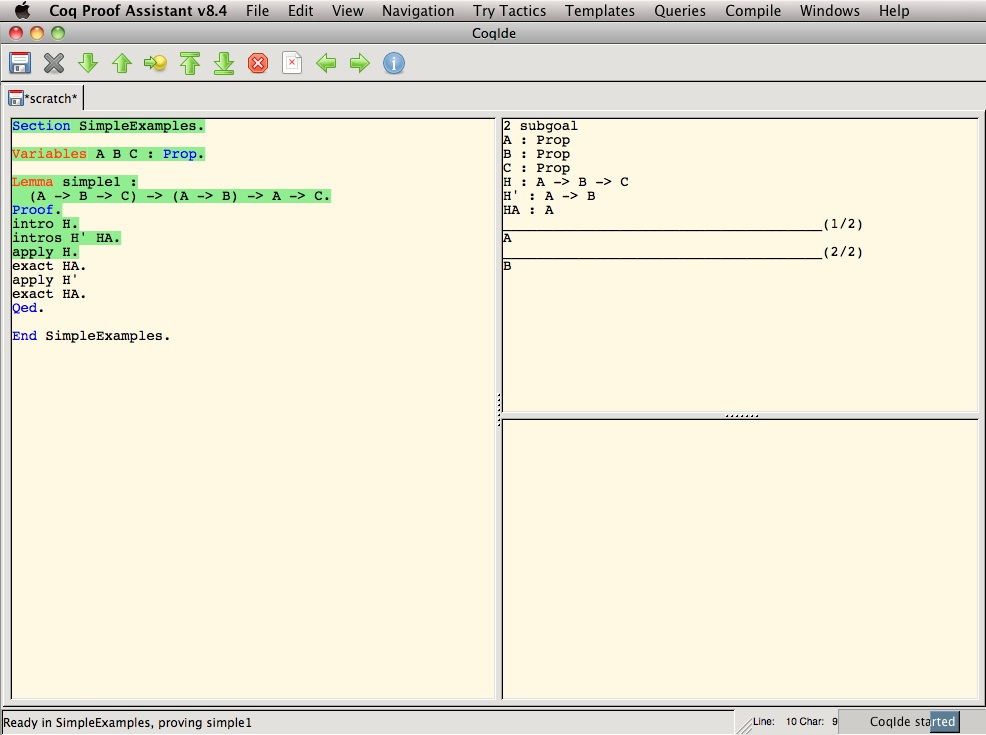
\includegraphics[width=\linewidth]{simple1_1.jpg}
  \caption{CoqIde, displaying the result of entering the tactic ``\texttt{apply H}'' in the top-right panel within the proof of \texttt{(A -> B -> C) -> (A -> B) -> A -> C}.}
  \label{fig:simple1_1}
\end{figure}

\begin{figure}[H]
  \center
  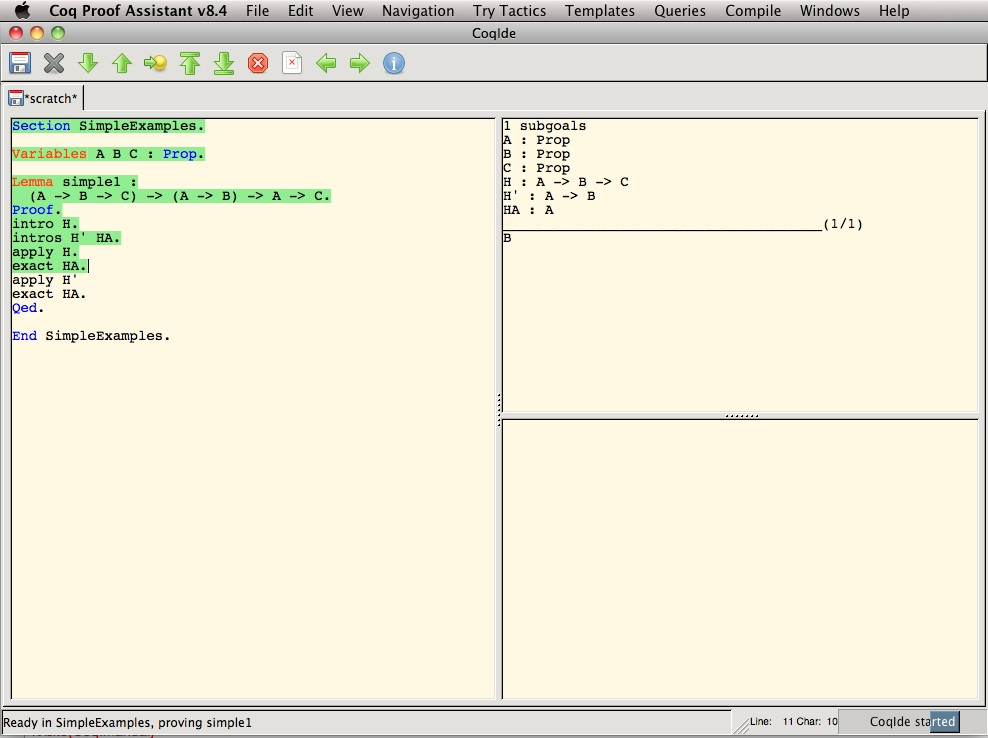
\includegraphics[width=\linewidth]{simple1_2.jpg}
  \caption{CoqIde after moving the end of the evaluated portion of the script forward by one sentence from the state shown in \autoref{fig:simple1_1}.}
  \label{fig:simple1_2}
\end{figure}


Users can extend the highlighted region both forward, to evaluate unhighlighted sentences, and backwards, to undo the effects of evaluation.  Users can instruct the system to extend the highlighting forward by one sentence, to retract it back by one sentence (though in the latest version of Coq, this sometimes will actually move the highlighting back several sentences), to extend or retract it to the cursor, to remove all of it (i.e. retract it to the start of the script), and to extend it to the end of the script.  These instructions can be entered into the system using toolbar buttons, drop-down menu items, or keyboard shortcuts.

\autoref{fig:simple1_1} and \autoref{fig:simple1_2} illustrate some of these points.  In \autoref{fig:simple1_1}, in the top right, we see the the result of evaluating ``\texttt{apply H}''.  In \autoref{fig:simple1_2}, we see the highlighting extended and the result of ``\texttt{exact HA} in the top right, namely the elimination of the first of the two subgoals in \autoref{fig:simple1_1} and the change in focus to the second.

This interface is problematic for novices trying to learn the effects of tactics.  Unfortunately, because the particular example being discussed is so simple, the severity of the problem may not be immediately apparent.  In \autoref{fig:simple1_1}, the two goals resulting from using the tactic ``apply H'' (the statement at the end of the highlighted region) appear to be displayed in the top right panel.  In fact, as mentioned earlier, only the first goal is fully displayed--the context for the second is not.  (In this case, the contexts for both are identical, but this is not always what happens).  To see the context of the second goal, probably the easiest, or at least most natural, thing for the user to do is highlight forward through all the tactics used to prove the first goal (just one tactic here, but potentially many in general).  It is up to the user to determine how far to highlight (or un-highlight, if looking at an earlier sibling goal) by keeping track of the list of goals in the top-right panel.  

In addition to the fact that users must move through the script to fully see siblings, no distinction is made between sibling and non-sibling goals in the list presented.  For instance, instead of using ``\texttt{exact HA}'' to transition to \autoref{fig:simple1_2}, the user could have used a tactic that produced two new goals.  The list of goals would then contain three goals, but only the first two would be siblings.  The user interface leaves it up to the user, however, to determine this by keeping track of the number of goals.\footnote{This sort of debugging gets even harder when one introduces proof automation features that allow combinations of basic tactic use attempts.}

Proof General does introduce a few features not present in CoqIde.  For instance, instead of making the highlighted region un-editable (``locking'' it), typing in the highlighted region retracts the highlighting back to the end of the sentence that is immediately before the cursor.  Unfortunately, these features are not really aimed at showing the effects of tactics.  A third user interface, \textit{Proof Web}\cite{ProofWeb} does make a serious attempt.  ProofWeb, for the most part, is a web-based version of CoqIde.  However, it has a major improvement, shown in the bottom right of \autoref{fig:proofweb}: a visualization of the partially completed proof tree.  

ProofWeb's display of the tree follows the convention where inferences are drawn with a horizontal line separating horizontally listed premises, above, from the conclusion below, and where each horizontal line is labeled with the name of the corresponding inference rule (or, in the case of Coq, by the corresponding tactic name) to the right of the line.  These inferences can be chained together so that the root of the proof tree is drawn at the bottom and the leaves are drawn at the top.  As an example, the portion of the proof tree constructed by ProofWeb that corresponds to ``\texttt{apply H}'' is shown in \autoref{fig:applyH} (the ellipses indicate that the child nodes are still unproved), and \autoref{fig:fulldisplaypartialtree} fully displays the partially completed tree.  The user is able to much more directly see the goal to which \texttt{apply H} is applied and the goals this application produces.

\begin{figure}[H]
  \center
  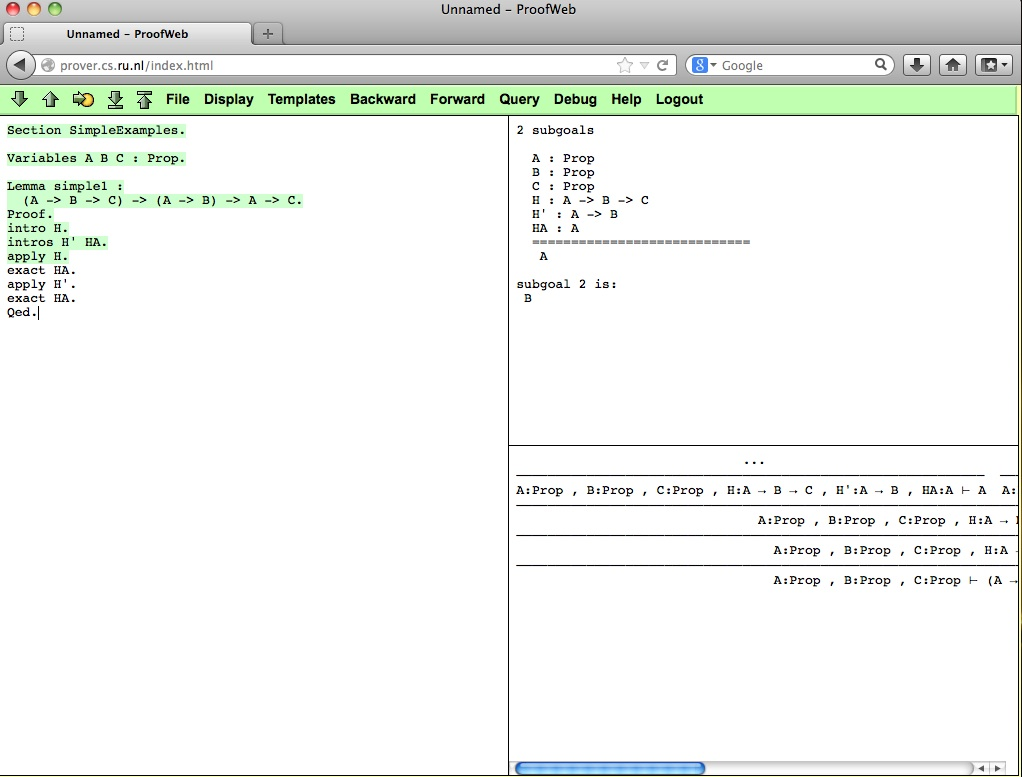
\includegraphics[width=\linewidth]{ProofWeb.jpg}
  \caption{ProofWeb, with a partial proof tree displayed in the bottom right.}
  \label{fig:proofweb}
\end{figure}



Unfortunately, as one can probably already tell, this sort of visualization does not scale particularly well.\footnote{Later in this document I provide what I hope is a clearly better alternative.} Contexts may may have dozens of items, many of which may be much longer than ``\texttt{H : A -> B -> C}'', and the number of nodes in the proof tree may also be very large.  As a result, the user may have to pan around the window to see the effect of a tactic; this is especially likely if one is looking at a tactic used near the root of the tree, since the width of the tree at its leaves forces apart nodes near the root.  Even if the user does not need to pan (ProofWeb has a feature that allows the tree to be displayed in a separate window, which can sometimes make panning unneccessary), the distances at which nodes with sibling and parent-child relationships must sometimes be placed may make it difficult for the user to compare such sequents and to determine if a direct relationship in fact exists (e.g. determine if two sequents that are printed next to one another are siblings or ``cousins'').  The latter task is possibly especially difficult using this visualization since it involves checking for gaps in co-linear line segments and the human brain tends to connect such lines.\footnote{This is the Gestalt law of ``good continuation; see, for instance, \cite{field1993contour}.}  The proof tree visualization, especially if there is a need to pan, is also not particularly helpful in showing the location of the current goal (users may have to search the leaves of the tree to find the leftmost ellipsis).

\begin{figure}[H]
  \center
  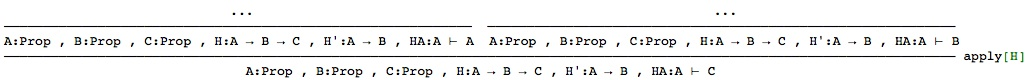
\includegraphics[width=\linewidth]{applyH.jpg}
  \caption{The portion of ProofWeb's tree visualization corresponding to the tactic ``\texttt{apply H}''.}
  \label{fig:applyH}
\end{figure}

\begin{figure}[H]
  \center
  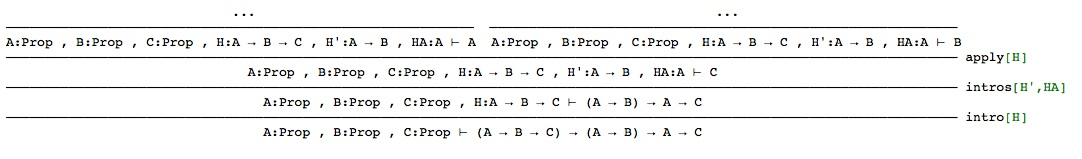
\includegraphics[width=\linewidth]{fullDisplayPartialTree.jpg}
  \caption{The partially completed tree from \autoref{fig:proofweb}, fully displayed.}
  \label{fig:fulldisplaypartialtree}
\end{figure}

The problems with current user interfaces that are discussed above are with respect to the scenario in which a novice user is inspecting an existing proof in order to determine the effects of various tactics under various conditions.  Many other scenarios with overlapping and related challenges also exist.  Such challenges include, but are not limited to,
\begin{itemize}
	\item locating particular items in a context (or in the larger environment)
	\item finding similar nodes in a proof tree
	\item deciding which tactic to apply
	\item keeping track of different proof attempts
	\item optimizing a proof or organizing a set of definitions, theorems and proofs for human understanding
	\item doing all these things efficiently. 
\end{itemize}



%%================================
\section{Coq User Interface Survey}
%%================================
Section \ref{currentUIproblems} described some usability problems that I, as a novice Coq user, noticed.  In this section, I describe an online survey (and its results) that Professor Juan Pablo Hourcade, Professor Aaron Stump, and I, in December 2011, invited subscribers to the Coq-Club mailing list to fill out.  This survey asked Coq users for their opinions and experiences regarding existing Coq user interfaces, and for their ideas regarding new interfaces.  Our motivation was both to validate our own ideas about new Coq user interfaces and to generate new ones.  We received 48 responses, including many detailed responses to the essay questions in the survey.

The survey consisted of 19 questions, of which 13 were multiple choice and the rest short answer or essay. The questions can be divided into three groups:  7 questions asking for background information on the respondent and how the respondent uses Coq, 9 questions asking for various ratings of the interface respondents use, and 3 open-ended questions directly related to the development of new user interfaces.  To these open-ended questions, we received many lengthy and thoughtful responses. \footnote{A more detailed survey report can be found at http://www.cs.uiowa.edu/~baberman/coquisuvey.html.}

The responses to the first group of questions showed a full range of (self-reported) Coq expertise levels, although a majority of responses indicated a high degree of expertise (on a scale going from 1=�novice� to 5=�expert�, 2 respondents rated themselves at level 1, 12 at level 2, 9 at level 3, 17 at level 4, and 8 at level 5).  9 respondents indicated they had been using Coq for less than 1 year, 27 for 1-5 years, 7 for 5-10 years, and 5 for more than 10 years.  Users of Proof General outnumbered users of CoqIDE 31 to 16.  24 respondents indicated using Coq for programming language or program verification research, 10 indicated using Coq for formalization of mathematics, and 8 indicated �teaching.� 

In the second group, to the question ``How satisfied are you with the interface you typically use?'', respondents gave a slightly positive average response (4.6 on a 1 to 7 point scale).  This was somewhat surprising to us at first, but it may have been an artifact of how the the question was asked.  For one thing, we did not present any sort of alternative interface, and current interfaces are, in fact, a significant improvement over the basic command prompt.  A second factor may be that many respondents have become accustomed to their current interface and may have viewed the question as asking how willing they would be to learn to use a new interface.  More than 25\% of respondents, however, did indicate some level of dissatisfaction.  Furthermore, answers to four questions revealed difficult tasks for users.  These questions asked users how difficult it is, using the interface they typically use, to 
\begin{itemize}
\item understand the relationships between subgoals, 
\item switch back and forth between potential proofs of a subgoal, 
\item compare similar subgoals, and 
\item tell what options for proving a subgoal are available. 
\end{itemize}
On a scale where 1=``Very Difficult'' and 7=``Very Easy'', the mean values for the answers to these questions were 2.74, 3.46, 2.35, and 2.57, respectively.   Responses to a fifth question, �How difficult is it for you to (mentally) parse Coq syntax?�, produced a mean value of 5.02 on the same scale, with only 4 responses indicating �Difficult� or �Somewhat difficult�.  Again, this may have been an artifact of the way the question was asked (e.g. to what the task might or might not in comparison be difficult was left unspecified).

In the third group, we received almost 4,500 words (total) in response to the questions  
\begin{itemize}
\item ``What information would you like to have more readily available when working with Coq?'',
\item ``What do you think are the hardest parts of learning interactive theorem proving with Coq?'', and
\item ``What advice/requests/ideas do you have for creating better Coq user interfaces?''
\end{itemize}
Because of this volume, I (very roughly) categorized the responses to each question.

For the first question, the first category was ``library documentation.'' Respondents noted that Coq's ``\texttt{SearchAbout}'' command is a little hard to use, that they would like more simple examples of using Coq commands, that theorem names are not very readable, and that they would like integration of documentation, a la the Eclipse IDE's javadoc support.\footnote{For the reader not familiar with Integrated Development Environments, they are essentially text editors with features specialized to programming in various languages.  Eclipse\cite{Eclipse} is one of the more popular IDEs for Java programming.}  The second category was ``available tactics''/``relevant lemmas, relevant definitions'': respondents wanted the names of previously proved statements they could apply and, additionally, whether a tactic could be used to automatically prove either the the current goal or its negation.  The third category was information on terms, e.g. the type of a term, the value to which it reduces, or other implicit information (such information can already be made available by using commands like ``\texttt{Check}'' and ``\texttt{Print}'').  The fourth category was proof structure, including information on the relationships both between goals within a proof and between theorems and definitions.  Miscellaneous responses included similarities between terms, differences between terms and expected terms, and tactic debugging with custom breakpoints.

For the question ``What do you think are the hardest parts of learning interactive theorem proving with Coq?'', the first category of response was type theory-- that learning the type theory behind Coq is one of the hardest parts.  The second category was with lack of good tutorials.  The third category was that there are numerous poorly documented commands (the need for simple examples was mentioned again).  Finally, the fourth category was proof readability, e.g. lack of support for mathematical notation and proof script organization.

For the question ``What advice/requests/ideas do you have for creating better Coq user interfaces?'', the first category was programming IDE features (e.g. auto-indentation, safe and correct renaming of identifiers, refactoring of tactics and groups of tactics, and background automation).  The second category was proof structure: representing proof structure by, for instance, grouping sibling goals, and allowing more flexibility to the order in which one works on goals.  The third category was syntax, which included having better ways to indicate where one wants to rewrite part of a term or where one wants to unfold a definition and automatic naming of hypotheses.  Some miscellaneous suggestions were to make more use of the mouse, avoid unnecessary re-execution of potentially long-running commands, and to have different editing and presentation tools.   

Even given the responses from self-described novice Coq users, the group of respondents is still heavily biased towards acceptance of arcane, complicated software.  The responses summarized above demonstrate that, even by this group, room for improvement is seen.


%=============================================================================
\chapter{CoqEdit, Proof Previews, and Proof Transitions}
\label{chapter:coqedit}
%=============================================================================

\section{Software Description}

\subsection{Basic CoqEdit}

The basic version of CoqEdit is a jEdit plugin providing a new user interface to Coq that is intended to imitate CoqIDE (see \autoref{fig:simple1_1}), Proof General, and ProofWeb (see \autoref{fig:proofweb}), described in \autoref{currentUIproblems}.  A significant difference between it and these previous user interfaces, however, is the use of two different shades of green, as seen in \autoref{fig:coqedit}:  all sentences highlighted with (some sort of) green are ones that have been successfully evaluated and cached, but the sentence highlighted with dark green has the result of its evaluation displayed in one of the two sub-windows on the right.  The user can move the dark green sentence around in this cached area.   This is in contrast to user interfaces like CoqIDE where there is only one shade of green, the evaluation result displayed on the right is always that of the last green sentence, and there is no caching of output.  Using CoqIDE, to check the result of an sentence evaluated earlier one must actually undo the evaluation of subsequent sentences (Proof General, like CoqEdit, caches evaluated sentence output, but has users hover over the evaluated sentence to see its result).  CoqIDE gets away with this because, frequently, re-evaluating a sentence is instantaneous.  However, this is not always the case, especially when using tactics that automatically search for proofs for goals (in general these are actually semi-decidable).  

\begin{figure}[H]
  \center
  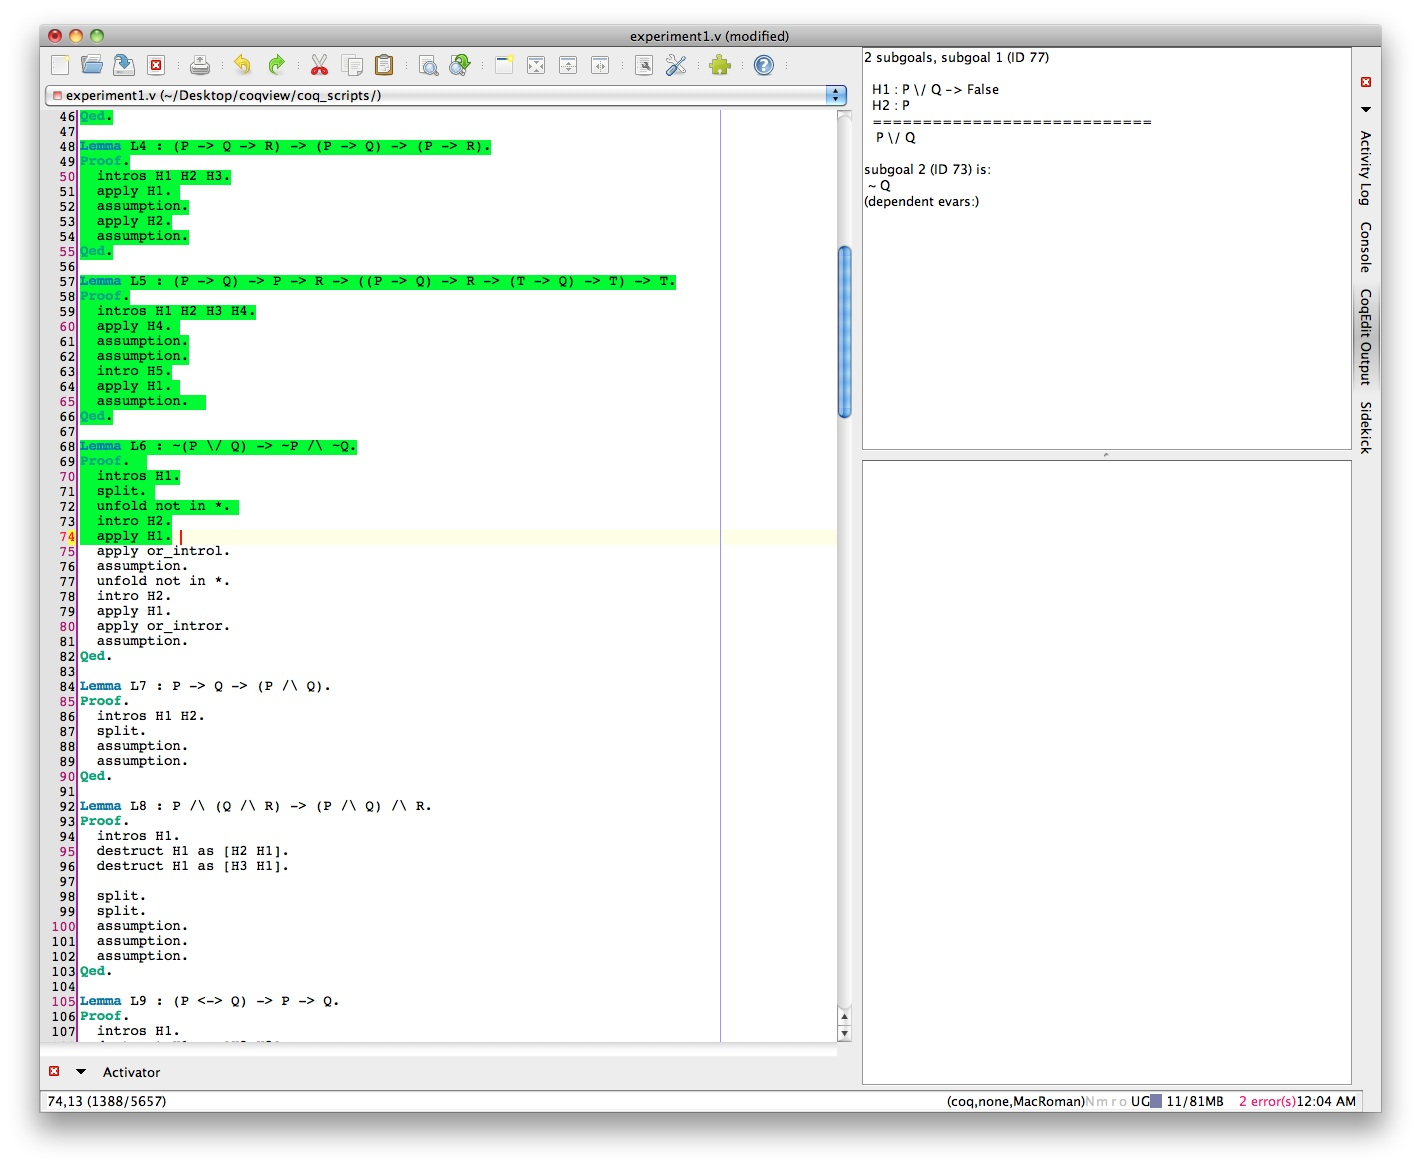
\includegraphics[width=\linewidth]{coqedit.jpg}
  \caption{The basic CoqEdit user interface}
  \label{fig:coqedit}
\end{figure}

To move the dark green highlighting forwards or backwards, one can select drop-down menu items (not shown in \autoref{fig:coqedit}, accessible through the ``CoqEdit'' submenu added to jEdit's top-level ``Plugins'' menu.  However, it is expected that generally users will use shortcuts which can be added and customized through the jEdit options menu (e.g. Ctrl-N for ``Forward one sentence'' and Ctrl-P for ``Back one sentence'').  There are 5 other menu items, which I hope are fairly self-explanatory:

\begin{itemize}
\item ``Show CoqEdit Output Panel,''
\item ``Go to cursor,''
\item ``Go to start,''
\item ``Go to end,'' and
\item ``Interrupt evaluation''
\end{itemize}

There are a few details regarding the user interface which may be unclear from the labels.  ``Forward one sentence'' moves the dark green highlighting forward within the light green section \textit{and}, when the dark green sentence is at the end of the green section, extends a purple section forward as seen in \autoref{fig:coqeditpurple}.  This purple section shows the sentence currently being evaluated and the subsequent sentences queued for processing.  

Frequently, evaluation occurs quickly enough that the purple section is invisible, but, as mentioned earlier, long-running and non-terminating commands may be encountered.  For these cases, the ``Interrupt evaluation'' menu item is provided which, in addition to interrupting any current sentence processing, removes all sentences from the queue of sentences to process and removes all purple highlighting.

\begin{figure}[H]
  \center
  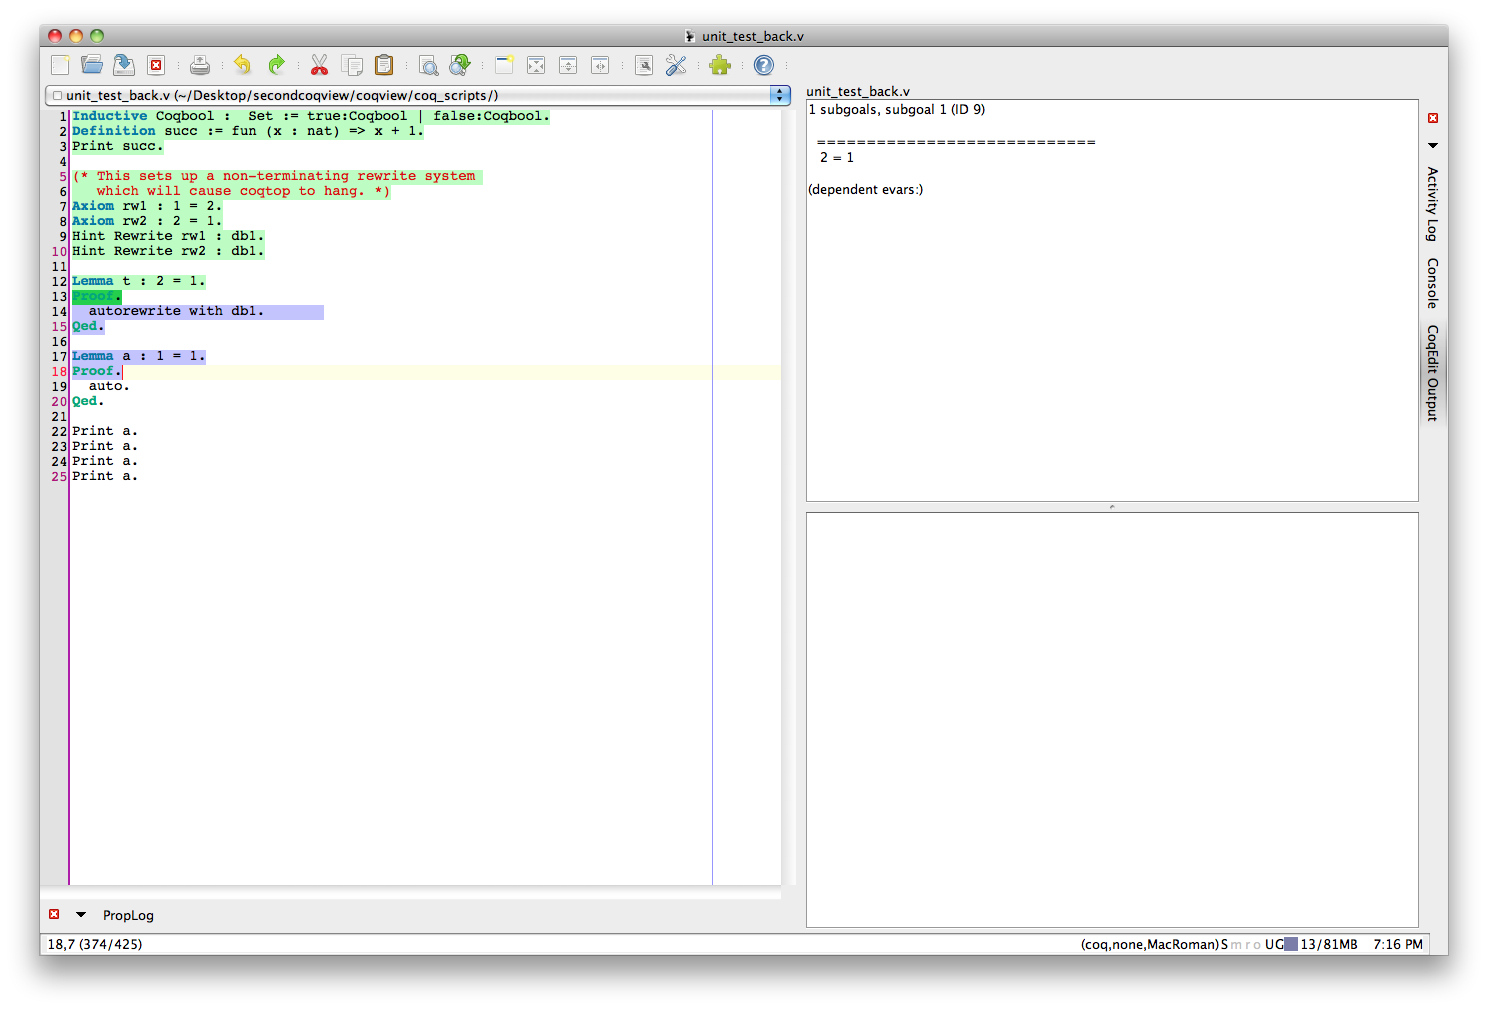
\includegraphics[width=\linewidth]{CoqEditProcessingVisualization.jpg}
  \caption{The basic CoqEdit user interface, when the first sentence highlighted with purple is being evaluated and the subsequent purple-highlighted sentences are queued for processing.  Thanks go to Harley Eades for providing this example of a non-terminating tactic.}
  \label{fig:coqeditpurple}
\end{figure}

The ``Interrupt evaluation'' menu item is not strictly necessary; an equivalent result could be achieved by inserting a character into the first purple sentence (and then deleting that character).  In general, typing into a highlighted region, green, purple, or red (used to indicate errors--see \autoref{fig:coqeditred}), undoes the evaluation/partial processing/queuing of the sentence into (from) which characters were inserted (deleted), and from all subsequent sentences.  To reflect this, the highlighting from these sentences is removed.\footnote{Typing into the sequence of tactics used to prove an earlier theorem or lemma actually causes the highlighting to be moved to just before the start of the lemma; this reflects the behavior of the underlying command line tool.}

\begin{figure}[H]
  \center
  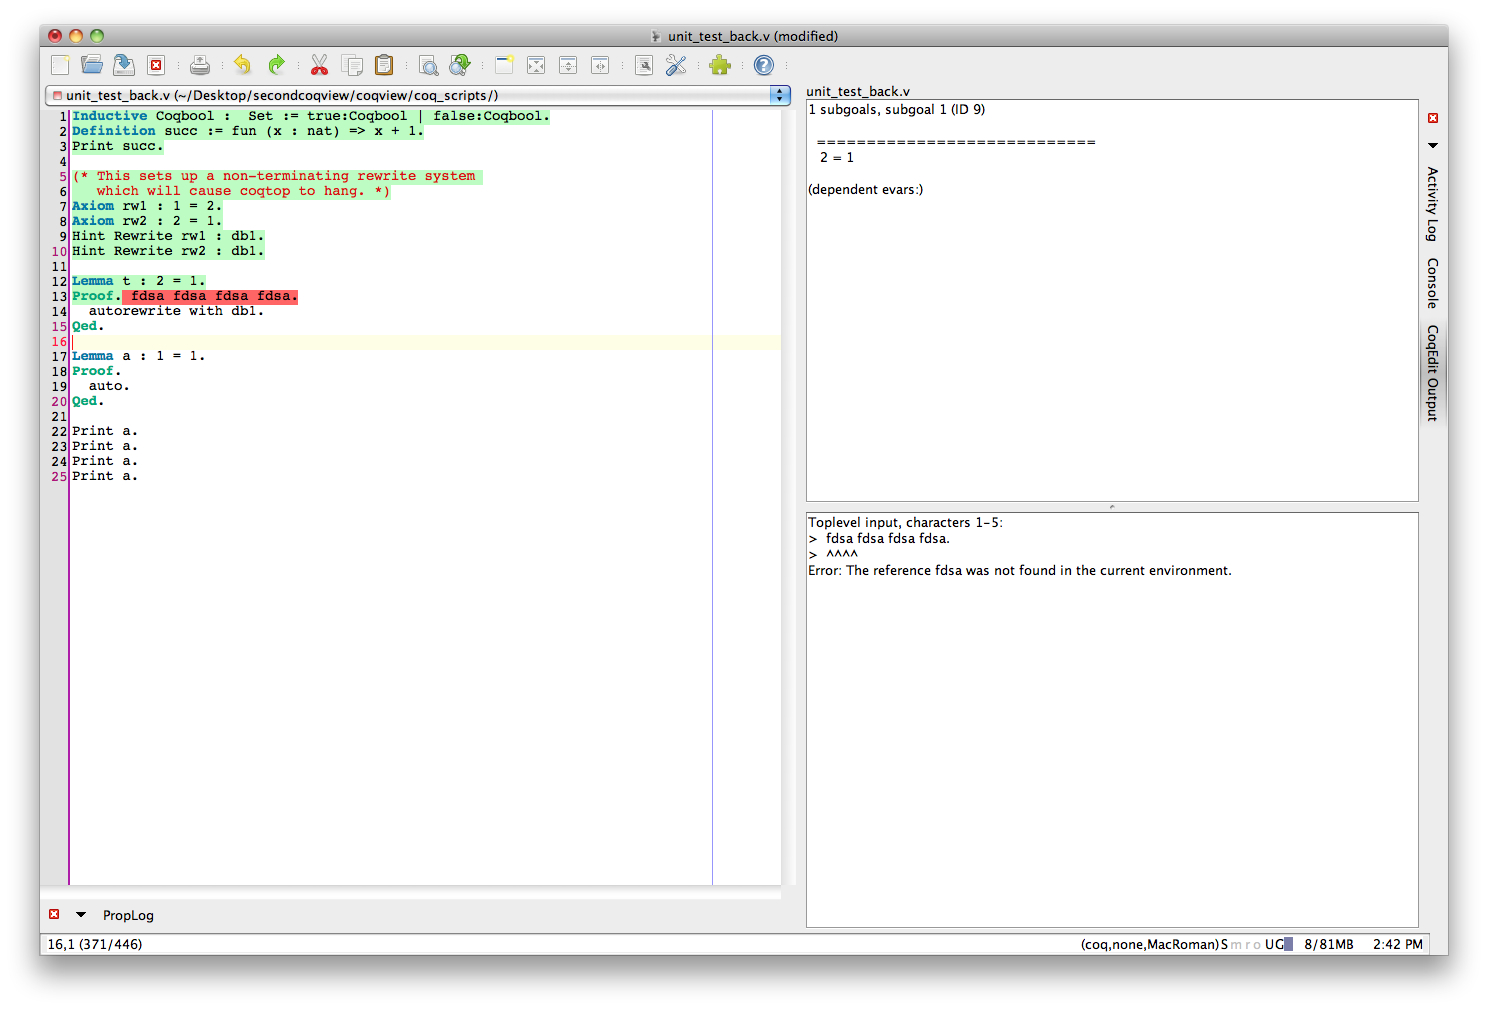
\includegraphics[width=\linewidth]{CoqEditErrorVisualization.jpg}
  \caption{The basic CoqEdit user interface, with an error-producing sentence highlighted in red.}
  \label{fig:coqeditred}
\end{figure}

To try to evaluate all sentences in the buffer, the user can use the ``Go to end'' menu item.  This of course may not always be successful since non-terminating and error sentences may be encountered, as in \autoref{fig:coqeditpurple} and \label{fig:coqeditred}.  Note that when an error is processed, processing stops, the sentences-to-process queue is emptied, and the highlighting is updated to reflect this.  Users are thus informed of incorrect proof attempts.  

``Go to end'' is effectively the same as repeated invoking ``Forward one sentence'' until there are no more sentences that can be queued for evaluation.  Similarly, ``Go to start'' is effectively the same as invoking ``Back one sentence'' repeatedly until the dark green highlighting is at the first sentence of the buffer, and ``Go to cursor'' attempts to move the dark green highlighting forwards or backwards to the sentence containing the cursor by invoking either ``Forward one sentence'' or ``Back one sentence'' repeatedly (when the first purple sentence is evaluated, the dark green highlighting will move to it).  

The navigational commands have the side effect of moving the cursor either to the end of the purple section (if moving forward) or to the end of the dark green sentence.  Moving the cursor in turn has the side effect of automatically scrolling the window so as to keep the cursor (and the most recently changed highlighting) visible.  This turns out to be highly convenient, allowing the user to avoid a large amount of manual scrolling.

As a jEdit plugin, CoqEdit lives in an ecosystem of other plugins which may have specified dependencies on one another.\footnote{If plugin A is specified (in its properties file) as depending on plugin B, then loading plugin A will automatically load plugin B (if it can be found among the downloaded plugins and is not already loaded) and unloading plugin B will (with a warning popup window) unload plugin A.}  One can view jEdit plugins that depend on CoqEdit as plugins to the plugin.  The next subsections describe two ideas for such plugins that were developed, and the next section describes how these ideas were tested with users in an experiment.

\subsection{Proof Transitions}

``Proof Transitions'' is a prototype for a proof tree visualization plugin for CoqEdit (or a similar plugin-based user interface for Coq or Coq-like proof assistants).  As a jEdit/CoqEdit plugin it would function in a manner similar to that of the proof tree visualization of ProofWeb (see \autoref{fig:proofweb}, \autoref{fig:applyH}, and \autoref{fig:fulldisplaypartialtree}):  as sentences of the buffer are evaluated and highlighted in green, nodes are added to the proof tree visualization.  However, the actual system, in its current prototype state at least, exists as a limited set of visualizations of complete proofs generated by.\footnote{More specifically, I reverse-engineered parts of Coq's tactic system and pretty printing system so that the fairly complex visualizations for several large propositional logic proofs could be generated relatively easily from an initial goal's syntax tree and a tree of tactics used to prove the initial goal.}   A fully developed plugin is beyond the scope of the research presented here--the goal of this research is to provide ideas for and insight into future work on such visualizations.\footnote{User interface development, particularly for proof assistants it seems, presents a chicken-and-egg problem:  back-end developers would like to avoid providing access to information that front-end developers don't use, but front-end developers have a hard time saying if they need access to that information until they test interfaces that use that that access.} 

\begin{figure}[H]
  \center
  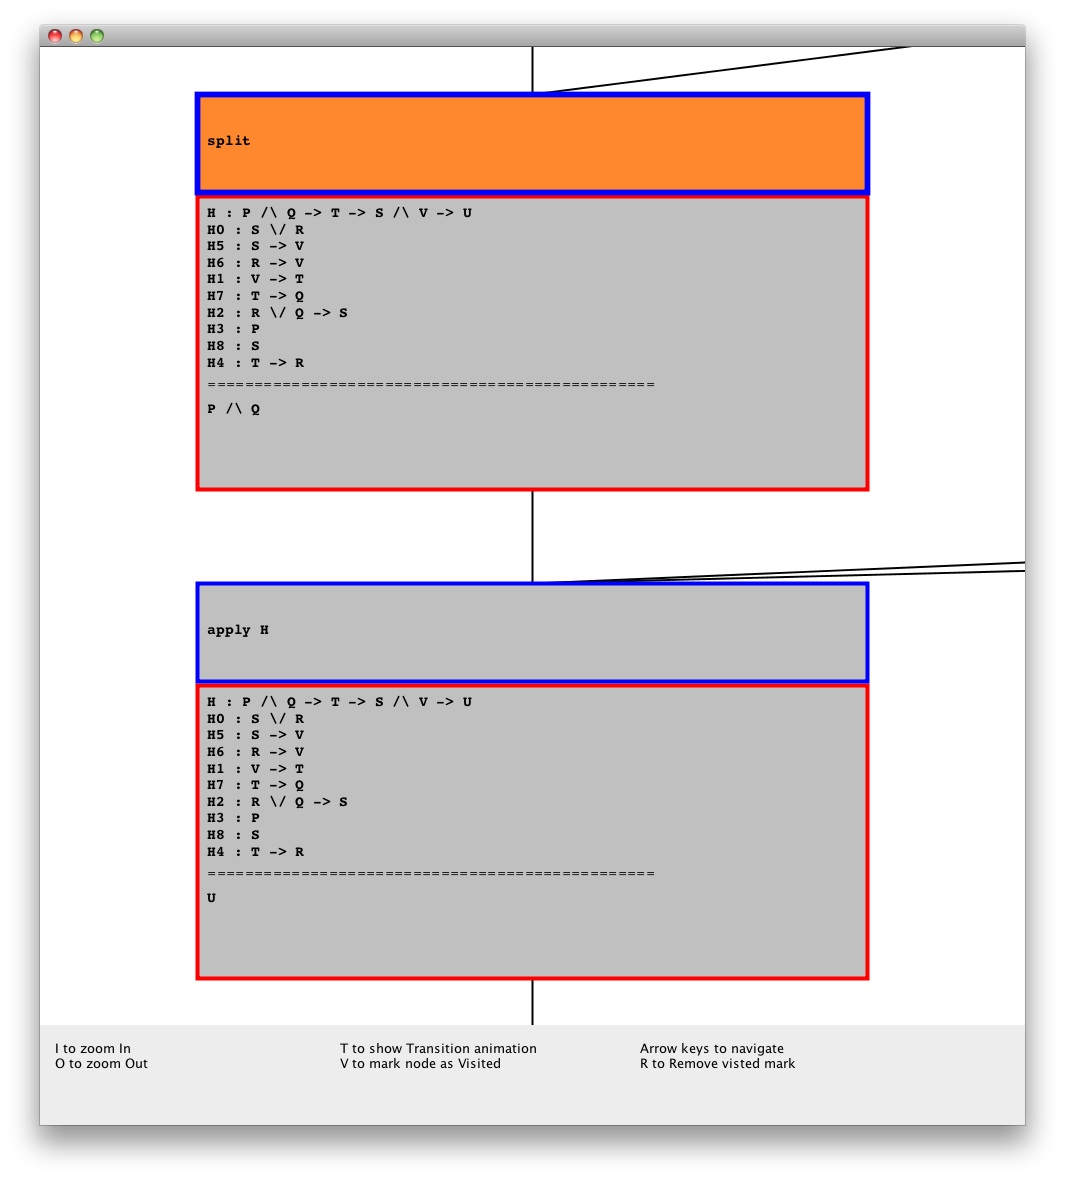
\includegraphics[width=\linewidth]{ptfirstchildzoomedin.jpg}
  \caption{}
  \label{fig:ptfirstchildzoomedin}
\end{figure}

Proof Transitions provides a zoomed-in and a zoomed-out level for viewing proofs. \autoref{fig:ptfirstchildzoomedin} shows the zoomed-in level.  Each node contains two parts:  the bottom box, outlined in red, contains the text of the goal, while the smaller top box, outlined in blue, contains the tactic used on that goal.

At the zoomed-in level two nodes are always visible:  the ``current'' node, which has its top box colored orange, and the current node's parent node, or, if the current node is the root node, the root node and its left-most child.  As one can see in \autoref{fig:ptfirstchildzoomedin}, the visualization follows the convention where parent nodes are displayed below their children. 

\autoref{fig:ptfirstchildzoomedout} shows how the proof tree is displayed when the user zooms out from the current node in \autoref{fig:ptfirstchildzoomedin}. At the bottom of the window in both \autoref{fig:ptfirstchildzoomedin} and \autoref{fig:ptfirstchildzoomedout} is a ``cheat sheet'' for the key presses used to manipulate the visualization.  From this, the user can learn or be reminded that the I and O keys are used to zoom in and out respectively.  Since there are only two zoom levels, pressing I while zoomed in, or O while zoomed out, does nothing.

\autoref{fig:ptsecondchildzoomedout}, \autoref{fig:ptthirdchildzoomedout}, and \autoref{fig:ptfourthgrandchildzoomedout} show what happens when one uses the arrow keys to move the current node to the sibling directly to right, twice, and then to the left-most child of the third of the three siblings (right arrow key, right arrow key, up arrow key).  Repeatedly using the left and right arrow keys will cycle through the current set of siblings.  

As shown, the visualization moves nodes so as to keep the current node above its parent (so that both the current node and its parent are visible when one zooms in).  To try to keep the shape of the tree relatively stable (i.e. to help users know which nodes are the same in \autoref{fig:ptfirstchildzoomedout}, \autoref{fig:ptsecondchildzoomedout}, \autoref{fig:ptthirdchildzoomedout}, \autoref{ptfourthgrandchildzoomedout}, for instance), the subtrees under the siblings, ``uncles'', ``great uncles'', etc., are each moved as a unit with each subtree getting its own allotment of space horizontally, \textit{and}, except for the parent of the current node, each parent node is kept centered above its left-most child (moving to the parent node from a child node other than the left-most requires shifting the subtree under the parent to the right to maintain this property).   

To make it even more clear that one is looking at the same set of nodes when one moves to a sibling, child, or parent node, the sliding around of nodes is animated over a fraction of a second.  \autoref{fig:ptdestructortransition} shows a snapshot of what moving to a sibling looks like when zoomed in.  Note that this animation does not limit the speed at which one can move from node to node (pressing, say, the right arrow key, while an animation is playing moves the nodes to where they would be at the end of that animation and then starts the new animation).

\begin{figure}[H]
  \center
  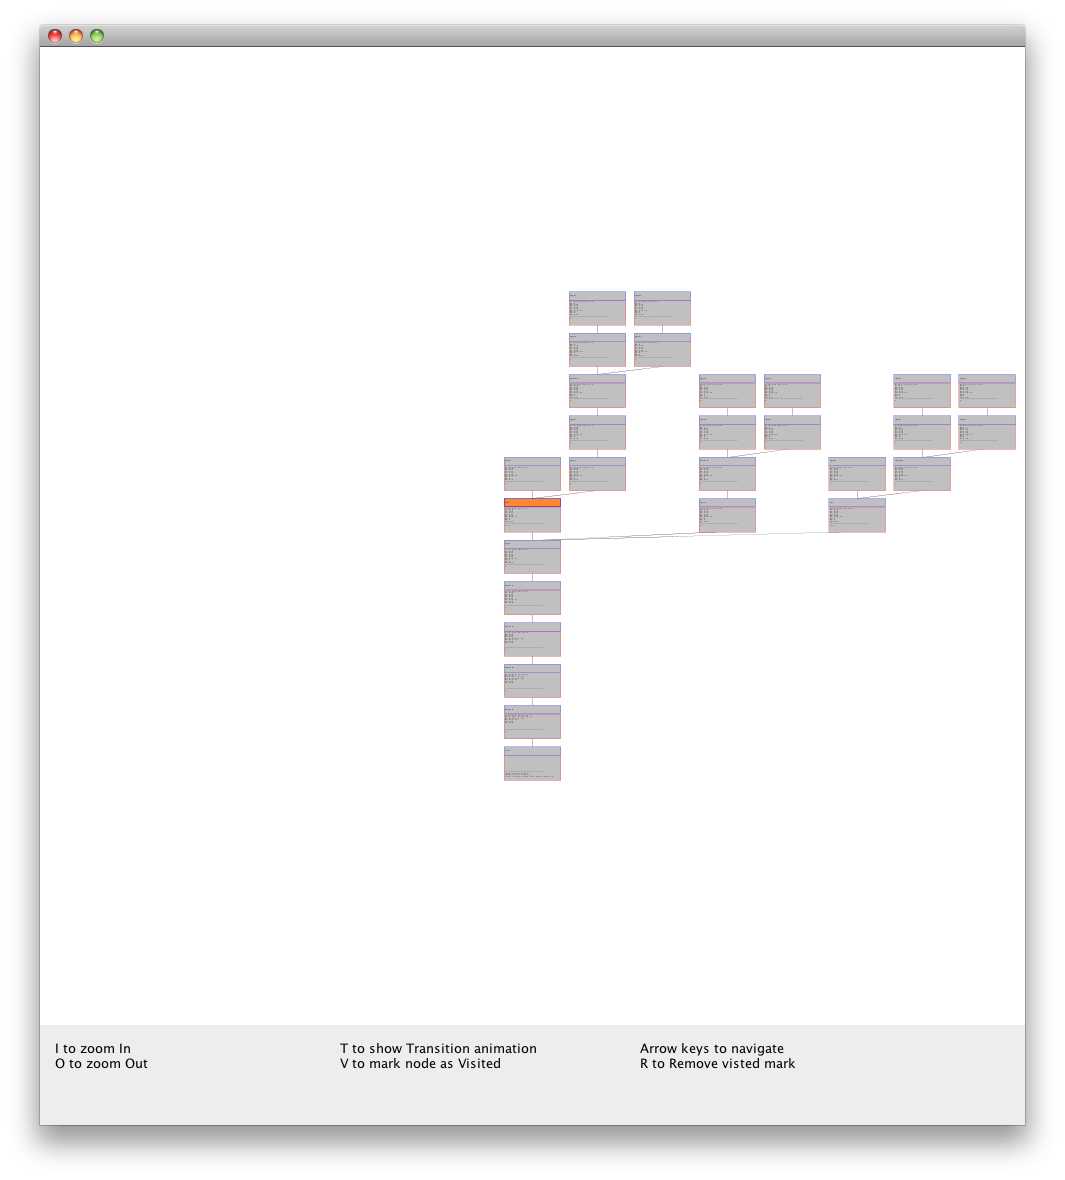
\includegraphics[width=\linewidth]{ptfirstchildzoomedout.jpg}
  \caption{}
  \label{fig:ptfirstchildzoomedout}
\end{figure}


\begin{figure}[H]
  \center
  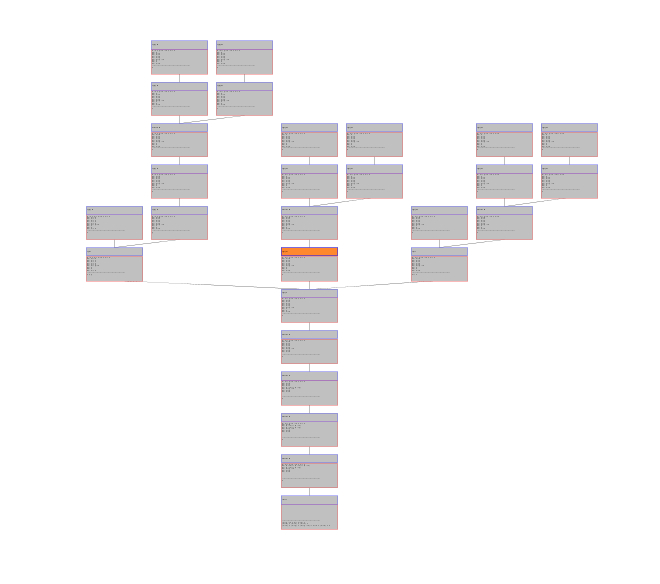
\includegraphics[width=.6\linewidth]{ptsecondchildzoomedout.jpg}
  \caption{}
  \label{fig:ptsecondchildzoomedout}
\end{figure}

\begin{figure}[H]
  \center
  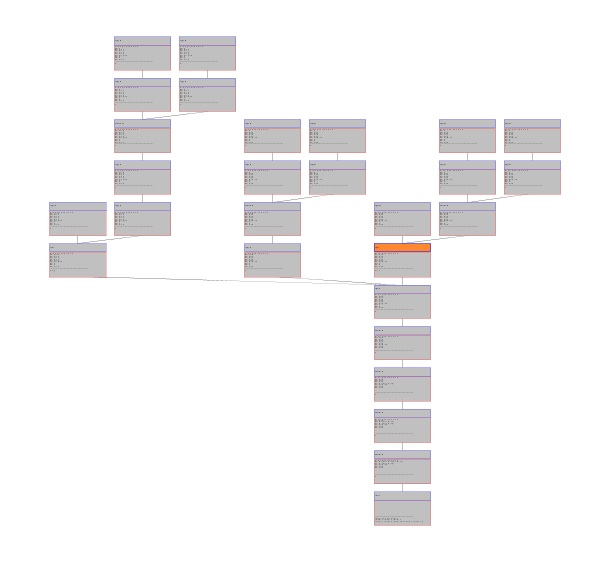
\includegraphics[width=.6\linewidth]{ptthirdchildzoomedout.jpg}
  \caption{}
  \label{fig:ptthirdchildzoomedout}
\end{figure}

\begin{figure}[H]
  \center
  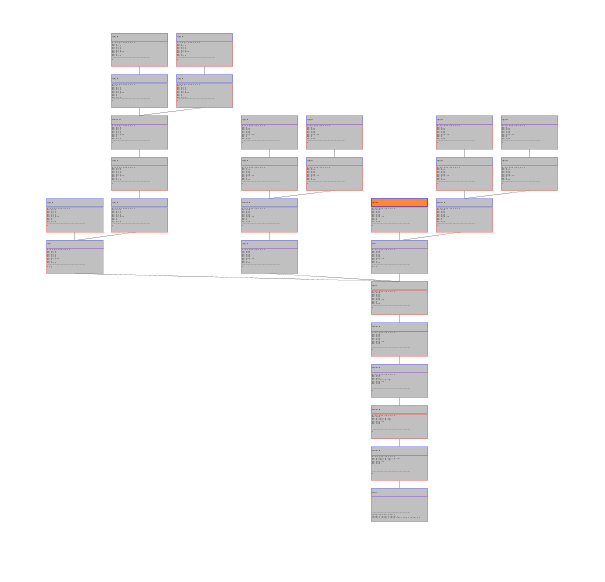
\includegraphics[width=.6\linewidth]{ptfourthgrandchildzoomedout.jpg}
  \caption{}
  \label{fig:ptfourthgrandchildzoomedout}
\end{figure}

\begin{figure}[H]
  \center
  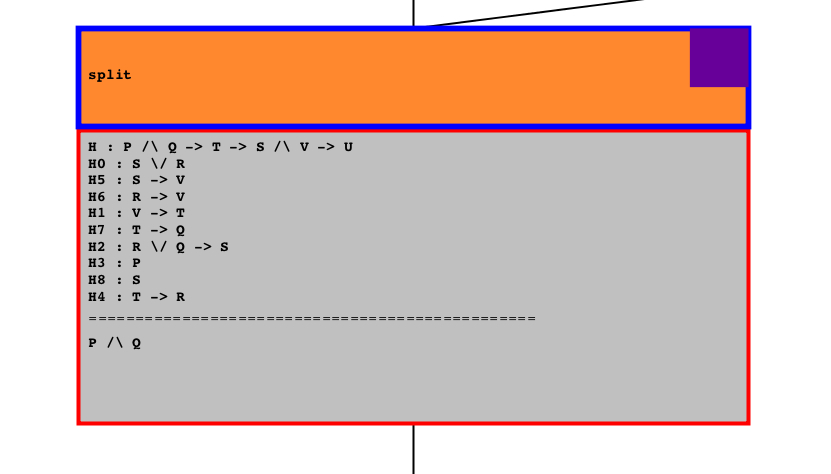
\includegraphics[width=\linewidth]{ptvisitednode.jpg}
  \caption{}
  \label{fig:ptvisitednode}
\end{figure}

One problem that became evident in initial ``pilot'' testing was that it was hard for users to keep track of which nodes they had inspected.  Users both visited nodes to which they had already been, thinking that they had not been there before, and they missed branches, thinking that explored them when in fact they had not.  To combat this problem, users are given the ability to add a small purple square to the upper right corner of a node to mark it as visited.  This is shown in \autoref{fig:ptvisitednode}; these purple squares are also visible when zoomed out.  Adding a purple square to the current node is accomplished by pressing the V key and removing a purple square (that might accidentally have been added) is a accomplished by pressing the R key.  These marks can be added and removed both while zoomed out and while zoomed in.  

In \autoref{fig:ptdestructand} through \autoref{fig:ptdestructor5} we see the other major feature of Proof Transitions---transition highlighting and animation.  Pressing the T key has the following effects:

\begin{itemize}
\item If the user is not already zoomed in, the visualization zooms in as if the I key were pressed.
\item The view shifts upwards so that the current node (which, recall, has the orange tactic box) is in the bottom half of the window and its left-most child is in the top half; see \autoref{fig:ptdestructand} and \autoref{fig:ptdestructor0}.
\item In the bottom node, text that disappears completely in every child node is highlighted in red.  In \autoref{fig:ptdestructand} this happens to be a conjunction symbol (``/\textbackslash'') whereas in \autoref{fig:ptdestructor0} through \autoref{fig:ptdestructor6} (which all show the same parent and set of children) it is a disjunction symbol (``\textbackslash/'').  This highlighted difference is actually the reason one child node is created by the ``destruct'' tactic seen in \autoref{fig:ptdestructand} in contrast to the the two nodes created by the same destruct tactic (albeit with a different argument) in \autoref{fig:ptdestructor0} through \autoref{fig:ptdestructor5}.
\item At the same time that the red highlighting is added to the parent node, green highlighting is added to each child node to mark text that is new in the child node (i.e. does not correspond in some way with text in the parent node).  Note that while there is green highlighting in \autoref{fig:ptdestructand}, since ``H7 : '' does not appear anywhere in the bottom node, there is no green highlighting in any of the child nodes in \autoref{fig:ptdestructor0} through \autoref{fig:ptdestructor5} since each child is entirely the result of removing and rearranging text from the parent node.
\item Blinking yellow highlighting is used to show where the tactic is finding or producing matching text.  For the sake of brevity, this is only shown in \autoref{fig:ptdestructor0} through \autoref{fig:ptdestructor5} and not in \autoref{fig:ptdestructand}.  Blinking occurs at a rate of two blinks per second and each matching pair gets five blinks.  Pressing T again, or moving to a different node, clears the red and green highlighting and stops the animation.
\end{itemize}


\begin{figure}[H]
  \center
  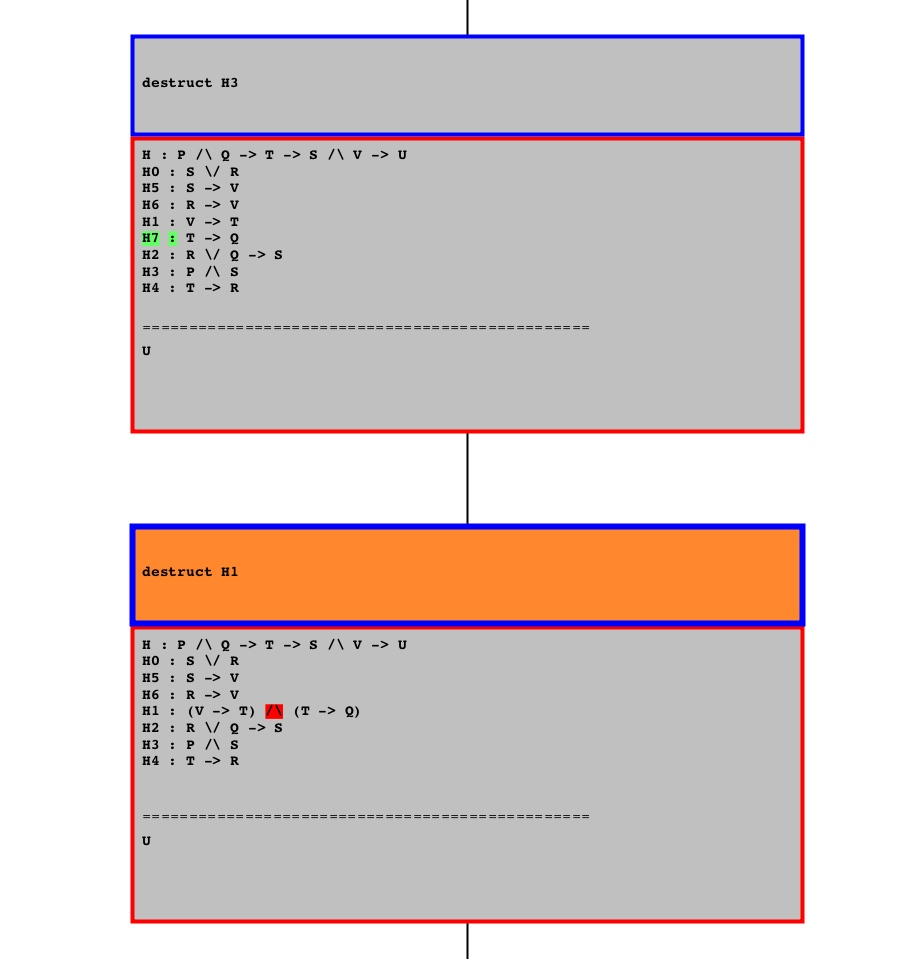
\includegraphics[width=\linewidth]{ptdestructand.jpg}
  \caption{The red highlighting marks text in the parent that does not occur in the (or, more generally, any) child node.  The green highlighting marks text occuring in the (each) child node that does not match text in the parent.  Note that the gray background, while perhaps somewhat unpleasing aesthetically, was selected so that all the highlighting colors would be visible.}
  \label{fig:ptdestructand}
\end{figure}


\autoref{fig:ptdestructor0} through \autoref{fig:ptdestructor5} document how the text-matching works in detail.  In \autoref{fig:ptdestructor0}, the animation ignores the child nodes altogether and uses the blinking yellow text to point out that the ``H0'' argument to the destruct tactic matches the H0 variable in the goal's context.  In \autoref{fig:ptdestructor1}, the blinking points out that the S on the left side of the disjunction in hypothesis H0 \footnote{As noted in the previous chapter, to be (more) pedantic we should say the S on the left side of the formula proved by the hypothesized proof labeled by H0} in the parent matches\footnote{By ``matches'' I really mean ``matches due to the way the destruct tactic works'' and not ``matches, perhaps by coincidence''. The animation does not aim to point out, for instance, that H0 and H8 in the first child's context are hypothesized proofs of the same formula.} the S of hypothesis H0 in the first child.  Similarly, in \autoref{fig:ptdestructor2} the blinking points out that the Rs match.  \autoref{fig:ptdestructortransition} is included to make clear that a fraction of a second is used to animate the movement to the second child node (and back to the first) that occurs between \autoref{fig:ptdestructor1} and \autoref{fig:ptdestructor2}.  \autoref{fig:ptdestructor3} through \autoref{fig:ptdestructor5} simply show the portions of the contexts that are unchanged between parent and children and that the goals also are unchanged (for the sake of brevity, the blinking highlighting used to show matching consequents between the parent and right node are not displayed as a figure in this document).

\begin{figure}[H]
  \center
  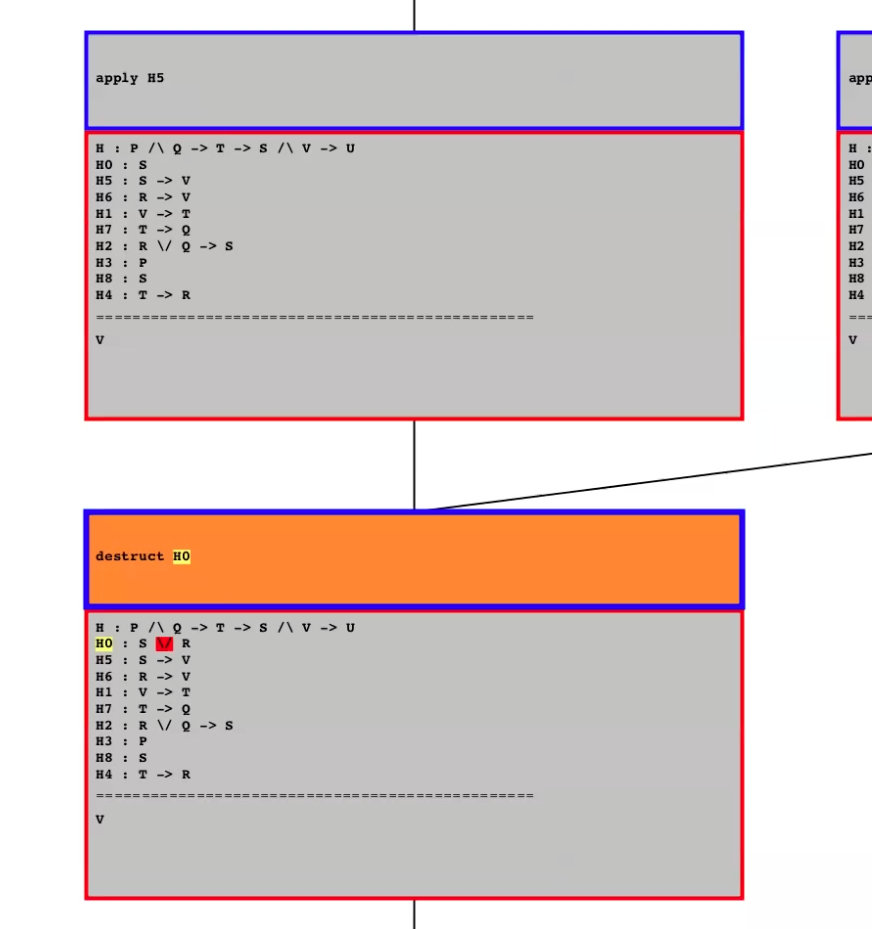
\includegraphics[width=\linewidth]{ptdestructor0.jpg}
  \caption{Blinking yellow text is used to show the context item matching the tactic argument.}
  \label{fig:ptdestructor0}
\end{figure}

\begin{figure}[H]
  \center
  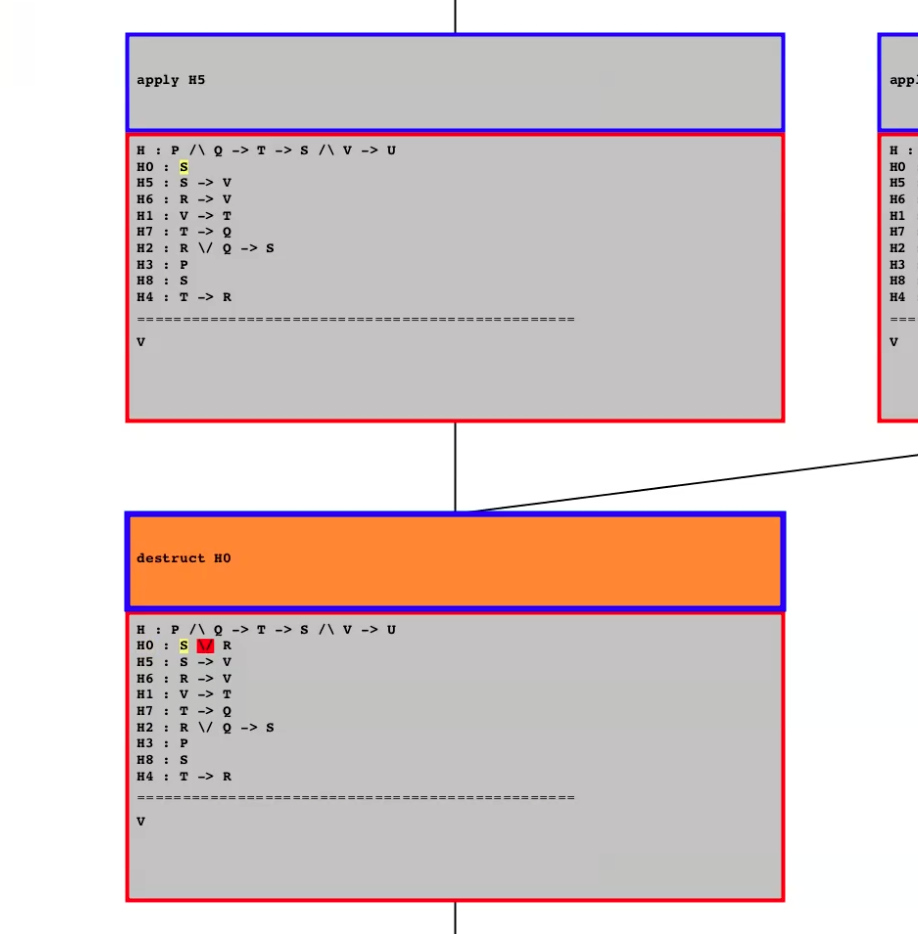
\includegraphics[width=\linewidth]{ptdestructor1.jpg}
  \caption{Blinking yellow text is used to show matching (sub)formulas in the parent and left child contexts.}
  \label{fig:ptdestructor1}
\end{figure}

\begin{figure}[H]
  \center
  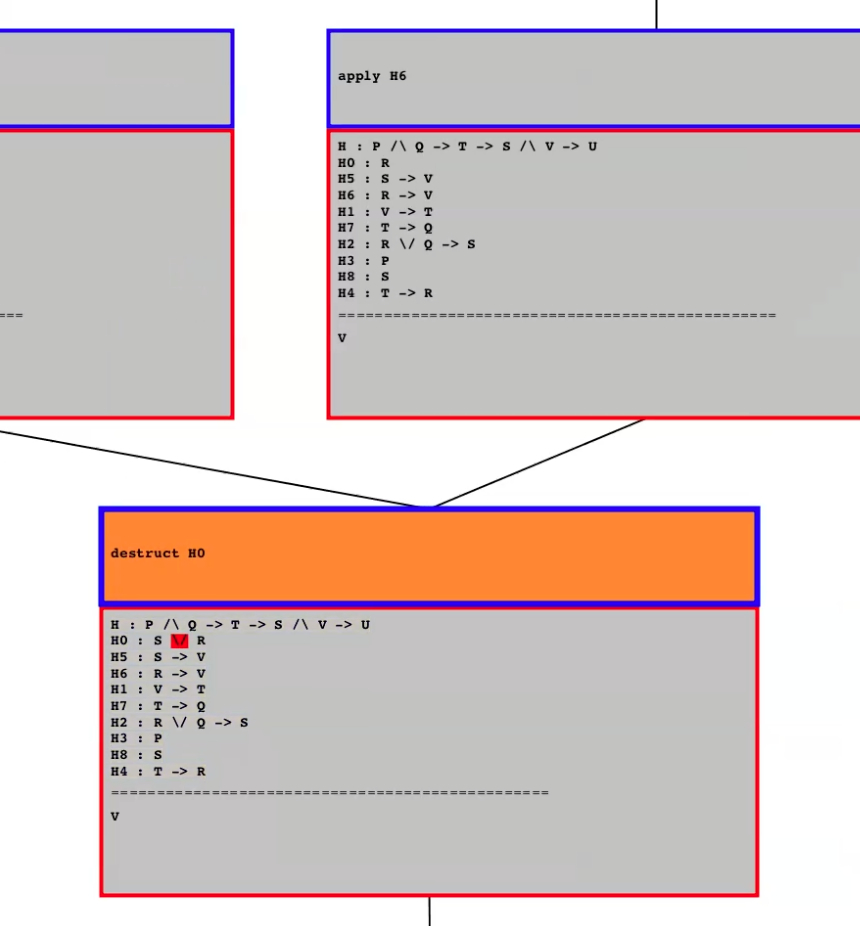
\includegraphics[width=\linewidth]{ptdestructortransition.jpg}
  \caption{The transition between \autoref{fig:ptdestructor1} and \autoref{fig:ptdestructor2} is animated}
  \label{fig:ptdestructortransition}
\end{figure}

\begin{figure}[H]
  \center
  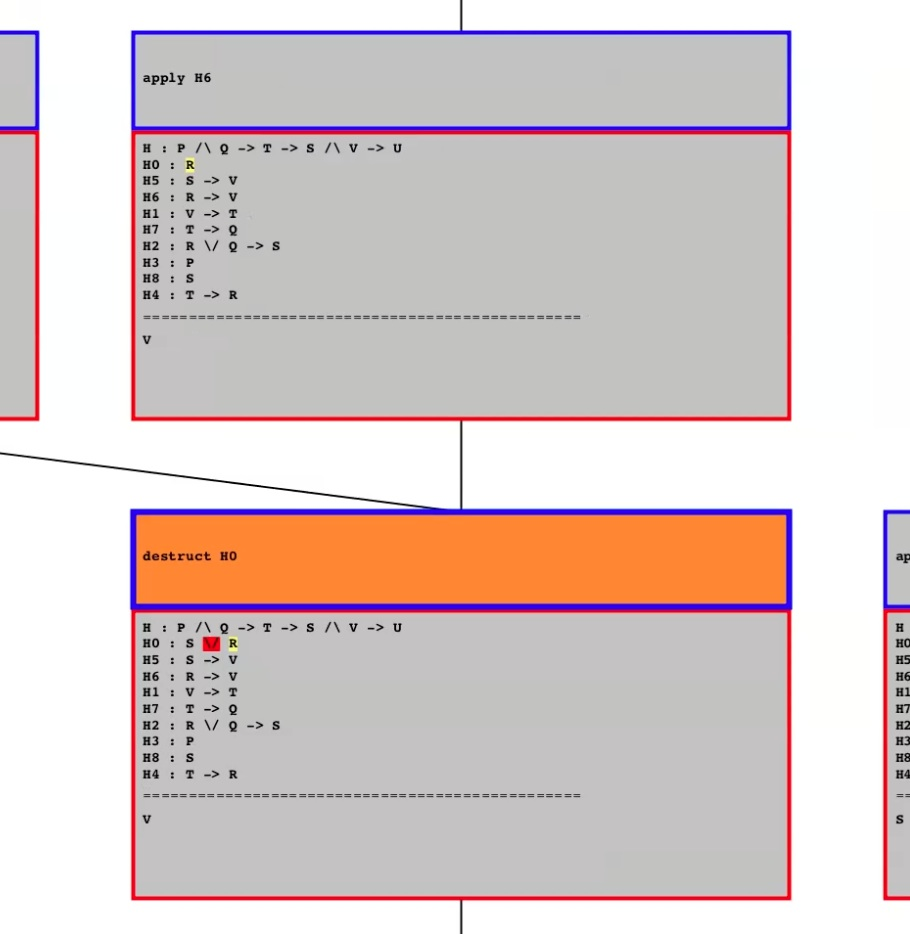
\includegraphics[width=\linewidth]{ptdestructor2.jpg}
  \caption{Blinking yellow text is used to show matching (sub)formulas in the parent and right child contexts.}
  \label{fig:ptdestructor2}
\end{figure}

\begin{figure}[H]
  \center
  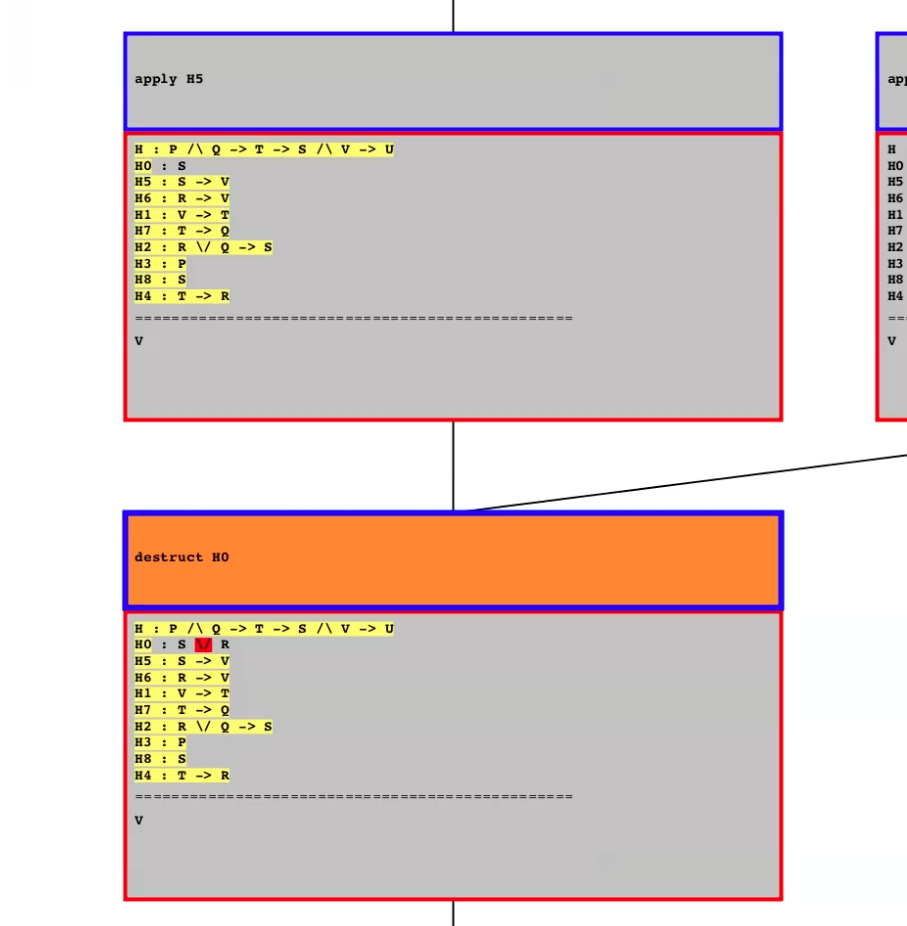
\includegraphics[width=.8\linewidth]{ptdestructor3.jpg}
  \caption{Blinking yellow text is used to show matching parts of the parent and left child contexts.}
  \label{fig:ptdestructor3}
\end{figure}

\begin{figure}[H]
  \center
  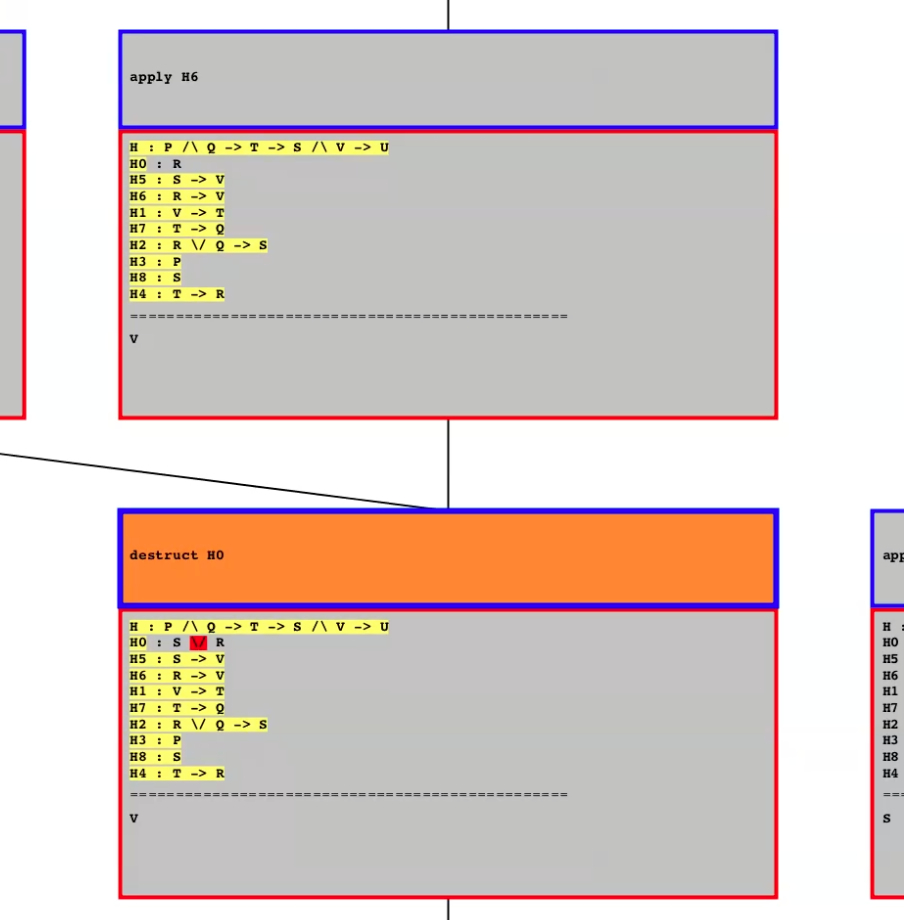
\includegraphics[width=.25\linewidth]{ptdestructor4.jpg}
  \caption{Blinking yellow text to show matching parts of the parent and right child contexts.}
  \label{fig:ptdestructor4}
\end{figure}

\begin{figure}[H]
  \center
  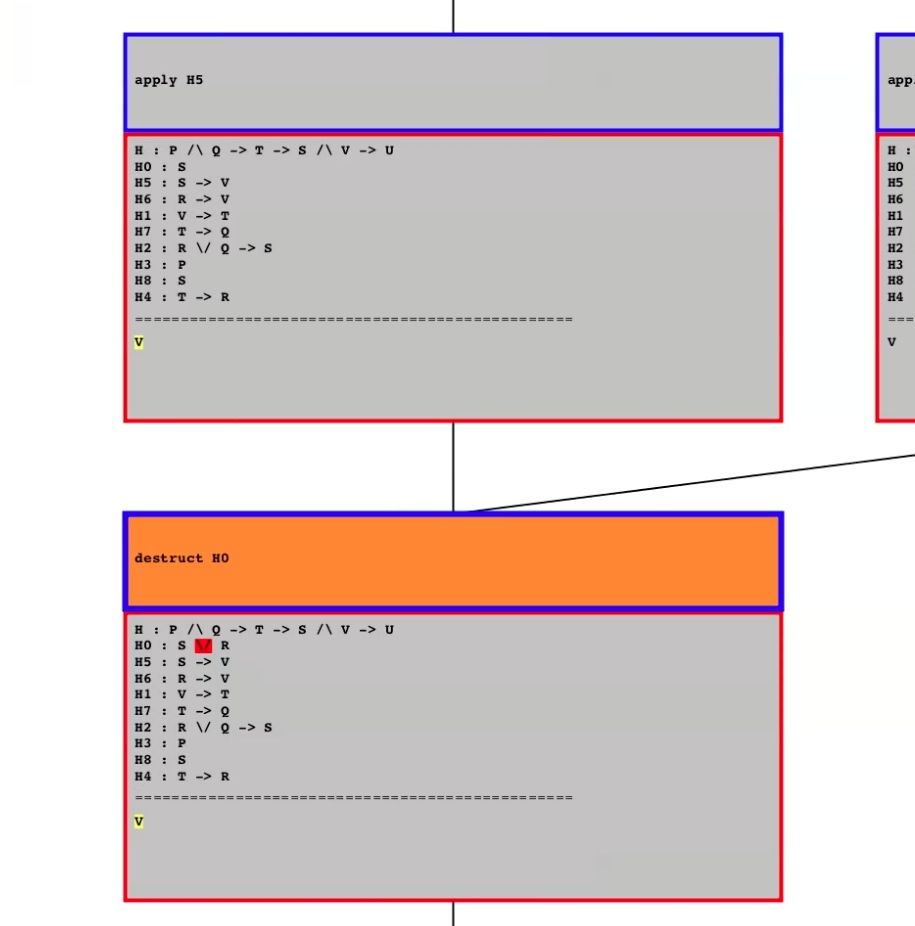
\includegraphics[width=\linewidth]{ptdestructor5.jpg}
  \caption{Blinking yellow text is used to show matching consequents for parent and left child nodes.  Blinking yellow text is also used to show matching consequents between the parent and the right child nodes.}
  \label{fig:ptdestructor5}
\end{figure}


%Goals/rationale for these designs?

What was the rationale for implementing these designs?  First, we wanted to confirm our hypothesis that a zoomable node-link view of a proof tree would help users understand the relationships between nodes and the effects of tactics--did a particular tactic produce two sibling goals or did it only produce one child goal?  We also envision(ed) such visualizations as potentially even more useful when further features are added (e.g. hiding less important branches when presenting a proof, cut/copy/paste of branches, version control for particular branches, bookmarking nodes, filtering nodes, etc.) and wanted to better understand how users deal with basic navigational issues as a preliminary step.

Second, with the transition highlighting and animation (i.e. blinking yellow text), we wanted to explore a potential way to make tactic effects easier to understand.  We were also interested in this feature because of its generalizability: one can think of this feature as a visualization of an extended version of the UNIX ``diff'' command wherein the actual editing commands, including copy as well as insert and delete, used to change document A into document B are recorded.\footnote{diff is a commonly used utility for comparing versions of documents, but only makes a best guess at where text was inserted or deleted and does not show where text was cut or copied and then pasted.}

\subsection{Proof Previews}

``Proof Previews'' is probably a more familiar sort of extension than Proof Transitions for most programmers as it is a variant of the standard ``Content Assist'' feature of Eclipse\cite{Eclipse} and other IDEs for programming.  Like Proof Transitions, it is currently quite limited compared to a fully developed plugin, but, unlike Proof Transitions, it is already set up as jEdit/CoqEdit plugin (giving evidence for the general feasibility of the modular interactive theorem prover user interface approach). 

In \autoref{fig:pp0} we see the result of invoking the ``Get Suggestions'' menu item in the jEdit plugin:  a popup listing of tactics that do not (immediately) produce errors when entered at the end of the green section.\footnote{In addition to creating the popup, it moves the dark green highlighting to the end of the green section.}  I expect (and observed in the experiment described in the next section) this to generally be invoked with a keyboard shortcut that, like the basic CoqEdit menu items, can be customized.\footnote{In the experiment, this was set to Ctrl-Space, matching the default for Content Assist in Eclipse.}


\begin{figure}[H]
  \center
  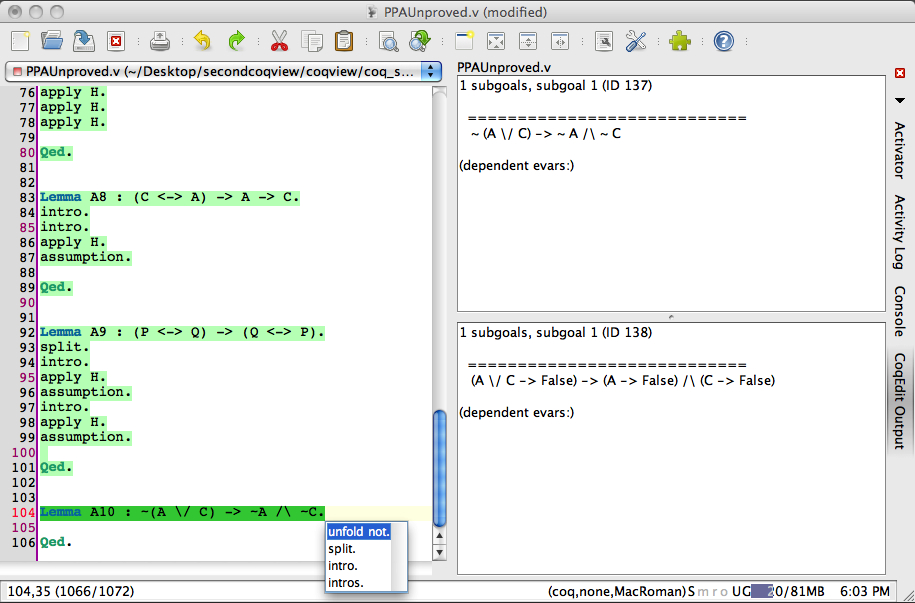
\includegraphics[width=\linewidth]{pp0.jpg}
  \caption{CoqEdit, with the Proof Previews plugin, after selecting the ``Get Suggestions'' menu item (or using an associated shortcut).  Note the popup window and the bottom-right sub-window showing the result of evaluating the tactic selected in the popup window.}
  \label{fig:pp0}
\end{figure}

The menu item only produces a popup when the last green sentence has the system in ``proof mode'' (i.e. after one has evaluated ``Lemma ... .'' but before evaluating the corresponding ``Qed.'')  A more fully developed plugin might give users the option of starting a lemma, for instance, outside of proof mode.   The menu item also does not appear if the plugin cannot find any tactics that would not immediately produce errors (which is not a guarantee that the current goal is impossible to prove).

In the bottom-right window in \autoref{fig:pp0} and \autoref{fig:pp1}, a "preview" of the result of entering and evaluating the selected tactic is displayed (hence the name ``Proof Previews'').  Users can use the arrow keys to move between popup menu items, and press the ESC key to close the popup window (using Proof Previews does not preclude normal tactic entry and evaluation).  

\begin{figure}[H]
  \center
  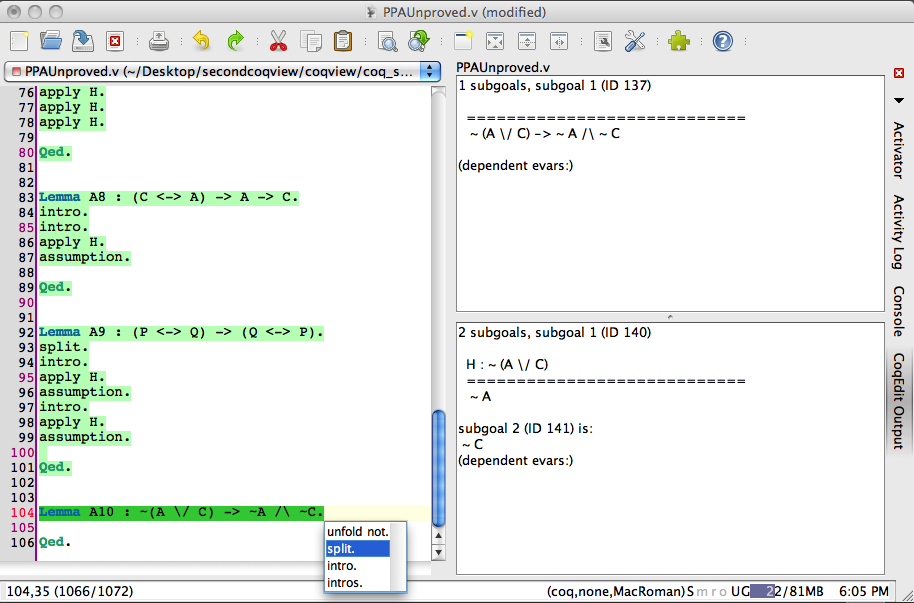
\includegraphics[width=\linewidth]{pp1.jpg}
  \caption{The result of pressing the down arrow from the state shown in \autoref{fig:pp0}.  Note that the bottom-right sub-window has changed to reflect the change in the popup window's selected item.}
  \label{fig:pp1}
\end{figure}

Pressing ENTER when the popup window is displayed will insert the selected tactic into the buffer on a new line at the end of the green region and will evaluate it (thus moving the dark green highlighting to the new tactic and the cursor to the end of the tactic's sentence); this is shown in \autoref{fig:pp2}.  As a result, some proofs can be completed simply by pressing Ctrl-Space (or whatever shortcut is used for the menu item), ENTER, Ctrl-Space, ENTER, Ctrl-Space, ENTER, etc., until there are no more subgoals.

The current version of Proof Previews, while sufficient for the experiment of the next section, is quite limited in its ability to search for potential tactics.  In particular, it does not look for theorems and lemmas from any libraries, or from the environment, to apply (it only tries to apply hypotheses in the context).  More advanced version of the plugin might search over indexed subsets of the standard library, hide any tactics producing goals with automatically provable negations, and/or do parallel searches.  The main goal of the current Proof Previews is to get a sense for how effective the user interface of an advanced
version might be.  Can Proof Previews improve the speed of text entry, and can it help users, particularly novice users, know their options options and make decisions?

\begin{figure}[H]
  \center
  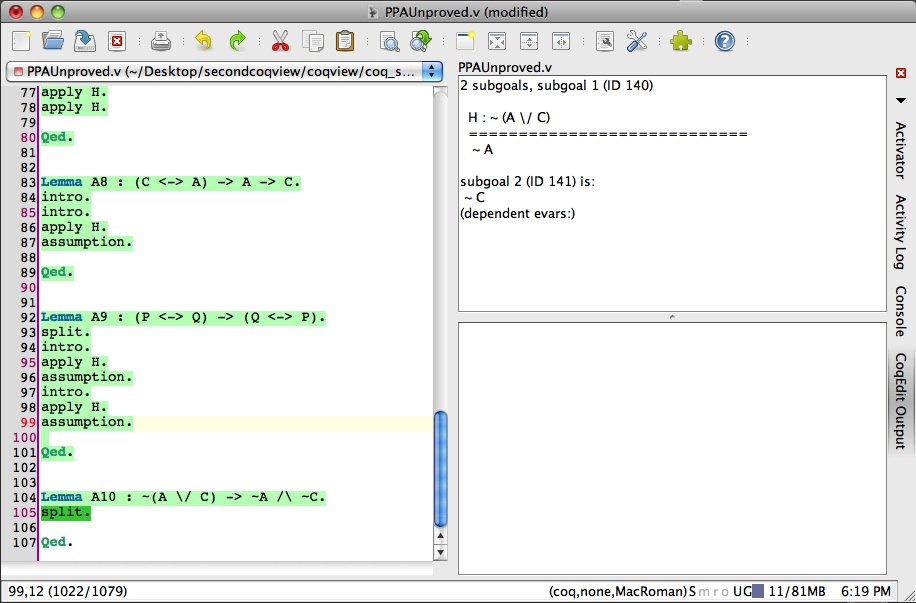
\includegraphics[width=\linewidth]{pp2.jpg}
  \caption{The result of pressing ENTER from the state shown in \autoref{fig:pp1}.  Note that the contents of the bottom-right sub-window in \autoref{fig:pp1} is now in the top-right sub-window and that the tactic that was selected in the popup window of \autoref{fig:pp1} is now inserted on a new line in the buffer and is evaluated.}
  \label{fig:pp2}
\end{figure}

\section{Experiment}

The goal of the experiment described below was to evaluate the effectiveness of Proof Transitions and Proof Previews in helping novice Coq users to understand proofs others have written and to write their own proofs.

\subsection{Experiment Design}

I conducted a 16-participant, counterbalanced within-subjects evaluation of Proof Transitions and Proof Previews.  The participants were recruited from University of Iowa Computer Science and Computer Engineering graduate and undergraduate classes and were required to have taken second semester undergraduate coursework.\footnote{Specifically, they were required to have taken 22c:019 ``Discrete Math'' and 22c:021 ``Data Structures'' at the University of Iowa, or equivalent coursework.}  The participants ranged in age from 19 to 37 (mean=23.4, standard deviation=4.1).  Three of the participants were women.  An additional 17th participant's data was excluded from the analysis as it included outlier values\footnote{Values greater than 3*(Q3-Q1) + Q3, where Q1 and Q3 are the first and third quartile values respectively, were considered outliers.}\footnote{In this particular case, the outlier values may have been attributable either to weak participant English fluency, or the fact that the participant was one of the first scheduled in the experiment.}

The experiment took place in a faculty member's office (only the participant and I were present). The single session with each participant generally lasted no more than two hours (though some participants opted to take extra time).  Participants were compensated with \$40.  During the session, participants used a 17-inch (1920 x 1200) MacBook Pro with a 2.8 GHz Intel Core 2 Duo Processor and 4 GB 1067 MHz DDR3 memory, running Mac OS X Snow Leopard.

The each session consisted of the following steps: 

\begin{enumerate}
%\item Participants were given a consent form describing the study, were given the opportunity to read it individually, and went over the most significant points (in particular, that they could stop their participation at any time without penalty) with the experimenter.  Consent was given verbally (no signature was obtained).\footnote{In accordance with the approval of the study given by the University of Iowa Institutional Review Board.}
\item After going through the consent process, participants filled out a payment form (where to send a compensation).
\item Participants filled out a demographic information form.  This asked for their ages, genders, levels of confidence in computer science skills and levels of confidence in logic skills (each on a 1-9 scale from ``Not at all'' to ``Very confident''), and which more advanced computer science courses they had passed.
\item Participants watched (and listened to) a training module.  This was a 50 minute video on proofs in propositional logic using Coq.  It covered the use of all tactics used in the rest of the experiment and presented the material using the basic CoqEdit user interface.  It also briefly introduced the Proof Transitions visualization features.  Only about 4 minutes were spent viewing proofs with the Proof Transitions interface, compared to about 40 minutes spent doing and viewing proofs using the basic CoqEdit interface (with the remaining time spent viewing slides).  Participants were reminded that they could take a break or ask questions at any time.
\item Participants were told (after watching the training video) that it would be a good time to take a break (not all did, and most who did took short < 5 minute breaks).
\item Participants were asked to navigate through two proofs that had already been completed and ``verbally explain how the proof works to the best of your ability''.  These were both presented using either the basic CoqEdit interface or Proof Transitions.  The proofs were both using only propositional logic with the first consisting of eleven nodes and the second consisting of twenty-eight nodes.  These explanations were recorded as screen-casts.
\item Participants were asked to again explain two (new) completed propositional logic proofs of the same lengths as the previous two.  If the participant had previously used Proof Transitions then in this step he used the basic CoqEdit interface and vice versa.  For this step and the previous, the four combinations (due to the two orders in which the two pairs of proofs were presented and the two orders in which the two interface types were presented) were balanced across participants.
\item Participants were asked to fill out the first two pages of a four page satisfaction and preferences questionnaire.  On the first page, participants were asked to give ratings for the first user interface they used on scales from 1 to 9 along the following axes:  terrible to wonderful, frustrating to satisfying, dull to stimulating, difficult to easy, inadequate power to adequate power, and rigid to flexible.  On the second page, participants were asked to rate the second interface they used in the same way.  On the second page they were additionally asked to give an overall preference (again on a 1 to 9 scale) between the first and second user interfaces, and a section for comments was given at the bottom of the page.
\item Participants were again prompted to take an optional break.
\item Participants were asked to prove as many of a set of 10 propositional logic lemmas as they could in a 15 minute period, using either just the basic CoqEdit or CoqEdit extended with Proof Previews.  With Proof Previews, participants were informed that they could press Ctrl-Space to get a popup window.  These lemmas all required between 3 and 10 tactics to prove.  Before starting, participants were given a paper ``cheat sheet'' reminder of tactics they could use and what the tactics would do, taken from the video tutorial.  The screen was again recorded during this and the next step.
\item Participants were asked to repeat the previous step with the user interface they had not used in the previous step and with a very similar set of ten lemmas.  (In a few cases the same lemmas were given with different variable letters).
\item Participants were asked to fill out the the last two pages of the satisfaction and preferences questionnaire.  These contained the same questions as on the first two pages.

 
\end{enumerate}

After the first eight participants, the above steps were refined:  

\begin{itemize}
\item Before starting the proof explanations, participants were presented with a guide for their explanations.  This stated ``For each tactic, please try to answer the following:  1) What nodes, if any, does the tactic produce from its goal?  2) How is each child node the same as or different from its parent?  3) Which text segments from the parent node get copied into the child nodes and where do they get copied to?''
\item Before starting the proof explanations, participants were also asked if they would like to set a timer for six minutes (generally sufficient) for each proof to ensure that the session did not last more than two hours.
\item Before starting the first of the two proof explanations using Proof Transitions, participants were asked to try using each of the features listed at the bottom of the window for at least the first three nodes in the first proof.
\item Before starting the first of the two proof explanations using the basic CoqEdit, participants were reminded of the shortcuts used to move forward and backward.
\item Before filling out each half of the satisfaction and preferences questionnaire, participants were given printed ``starter questions'' for the comments section.  Starter questions common to both comment sections were ``Why did you prefer one interface over the other?'', ``Were there any improvements that you think could be made to either interface?  How significant would these improvements be?'', ``Was there anything in particular that was confusing about either interface?'', and ``Were there any features of either interface that you could do without?  Were there any that were especially helpful?''.  Specific to the proof interpretation questions were ``In the interface with the boxes and flashing highlighting, was having to back away from leaves manually, instead of automatically moving to the next branch, something that made a big difference?'' and ``In either interface, did you find yourself getting `lost'?''  Specific to the theorem proving questions was ``When using the popup window, did you find the preview of the result, in the bottom right, helpful?''
\item Before using Proof Previews, participants were walked through how to use the extension to create a three tactic proof of A \ra (B \ra C) \ra (A \ra C) \ra C.  They were also told to use Proof Previews exclusively.
\end{itemize}


\subsection{Results}

Probably the most disappointing result turned out to be Proof Transitions' transition highlighting and animation, which went largely unused (possibly for the reasons discussed in the next subsection).  However, other results were more positive.

\begin{table}
\begin{tabularx}{\textwidth}{ |X|X|X| }
  \hline
                                                                      & \bf Average & \bf Std Dev \\
  \hline
  \bf Terrible to Wonderful                             & 6.1  & 1.5 \\
  \hline
  \bf Frustrating to Satisfying                         & 5.4 & 1.5   \\
  \hline
  \bf Dull to Stimulating                                  & 6.5  & 1.1   \\
  \hline
  \bf Difficult to Easy                                      & 5.9  & 2.5  \\
  \hline
  \bf Inadequate Power to Adequate Power  & 6.3  & 2.3  \\
  \hline
  \bf Rigid to Flexible                                    & 6.3  & 1.9    \\
  \hline
  
\end{tabularx}
\caption{Satisfaction and preferences questionnaire average results for proof interpretation using Proof Transitions.  Values go from 1 to 9 (e.g. a 9 for a Terrible to Wonderful rating would mean completely wonderful).}
\end{table}
\label{tab:ptratings}

\begin{table}
\begin{tabularx}{\textwidth}{ |X|X|X| }
  \hline
                                                                      & \bf Average & \bf Std Dev \\
  \hline
  \bf Terrible to Wonderful                             & 6.8   & 1.2 \\
  \hline
  \bf Frustrating to Satisfying                         & 7.0 & 1.6   \\
  \hline
  \bf Dull to Stimulating                                  &  5.7 & 2.0   \\
  \hline
  \bf Difficult to Easy                                      &  7.1 &  2.1 \\
  \hline
  \bf Inadequate Power to Adequate Power  &  7.1 &  1.6 \\
  \hline
  \bf Rigid to Flexible                                    &  6 & 2.1    \\
  \hline
  
\end{tabularx}
\caption{Satisfaction and preferences questionnaire average results for proof interpretation using the basic CoqEdit interface.  Values go from 1 to 9 (e.g. a 9 for a Terrible to Wonderful rating would mean completely wonderful).}
\end{table}
\label{tab:nonptratings}

\autoref{tab:ptratings} and \autoref{tab:nonptratings} show the questionnaire rating averages for the proof interpretation/explanation with Proof Transitions and the basic CoqEdit interface respectively.  The differences were statistically significant only for the Frustrating to Satisfying axis.  The overall preference rating average, again on a 1 to 9 scale but this time with 1 indicating preference towards Proof Transitions and 9 indicating preference towards the basic CoqEdit interface for explaining proofs had an average of 5.8.  This was, however, not a statistically significant difference from the middle value of 5.  In fact, five of the participants gave a number less than 5, indicating a preference towards the Proof Transitions interface, and one more gave a value of 5, indicating no preference.

%Comments on PT vs basic

Comments on Proof Transitions versus basic CoqEdit included:

\begin{itemize}
\item ``I am a programmer, so I lean towards the [basic CoqEdit interface].  However, if I was to present my findings I would use the [Proof Transitions] interface because people would find it more clear on how the flow of logic works.'' ... ``[In Proof Transitions] I found myself wanting to click left and right when I needed to move up or down''
\item ``[In Proof Transitions] too much zooming in and out required gets little confusing sometimes.  However, the animation of 2nd user interface is really cool and makes it intuitive''
\item ``[Proof Transitions] was confusing in the sense which way the proof flows''
\item ``I thought by watching the video that the first UI would be easier to understand b/c more time was spent on it, but the visual one was more intuitive''
\item ``I really liked the transition mode of [Proof Transitions], it really helped me visualize the process of solving the proofs.  I also enjoyed the first, but the second was a far better visual tool which helped me since I'm more of a visual learner.  However, in [Proof Transitions] I did get lost some times when the proof really branched out.  Finally, for the [basic CoqEdit user interface] I liked how it listed all the current subgoals which helped out since there were some times I got confused in [Proof Transitions] due to forgetting whether a subgoal had been proved yet or not.''
\item ``The first interface is very confusing, as it is not made clear that when the path branches, new goals have been added.  Not being able to see all the goals at once makes it difficult to know how far you have progressed in the total proof.''
\item ``[With Proof Transitions] I found [it] easy to get lost.''
\item ``Would like a zoom level somewhere between all the way out and all the way in.''
\item ``[Proof Transitions] allow us to view the proof more easily so that we can understand it better, but it is difficult to edit it.''
\item ``[The basic CoqEdit user interface] is straightforward''...``[Proof Transitions could] have more scales when do[ing] the zoom in/out''...``For [Proof Transitions], if the proof is complicated, the diagram could be very frustrating''...``If there is a mini map, it would help''.
\item ``I wanted both for harder proofs.  You can get lost in the leaf paths.  I prefer working with the text, out of habit, but the visual helped for backtracking.''
\item ``Should do [Proof Transitions zoom out feature] in steps until user is comfortable in reading text''...``I forgot to use `visit' option.  Might proved to be helpful.''

\end{itemize}

%Ratings for PP

\begin{table}
\begin{tabularx}{\textwidth}{ |X|X|X| }
  \hline
                                                                      & \bf Average & \bf Std Dev \\
  \hline
  \bf Terrible to Wonderful                             & 8.2  & 1.1 \\
  \hline
  \bf Frustrating to Satisfying                         & 8.0 & 1.3   \\
  \hline
  \bf Dull to Stimulating                                  & 7.4  & 2.1   \\
  \hline
  \bf Difficult to Easy                                      & 8.4  & 1.1  \\
  \hline
  \bf Inadequate Power to Adequate Power  & 8.3  & 0.7  \\
  \hline
  \bf Rigid to Flexible                                    & 7.6  & 1.7    \\
  \hline
  
\end{tabularx}
\caption{Satisfaction and preferences questionnaire average results for theorem proving using Proof Previews.  Values go from 1 to 9 (e.g. a 9 for a Terrible to Wonderful rating would mean completely wonderful).}
\end{table}
\label{tab:ppratings}

\begin{table}
\begin{tabularx}{\textwidth}{ |X|X|X| }
  \hline
                                                                      & \bf Average & \bf Std Dev \\
  \hline
  \bf Terrible to Wonderful                             & 7.1   & 1.5 \\
  \hline
  \bf Frustrating to Satisfying                         & 6.9 & 1.7   \\
  \hline
  \bf Dull to Stimulating                                  &  7.2 & 1.2   \\
  \hline
  \bf Difficult to Easy                                      &  6.4 &  1.9 \\
  \hline
  \bf Inadequate Power to Adequate Power  &  6.8 &  1.8 \\
  \hline
  \bf Rigid to Flexible                                    &  6.7 & 2.1    \\
  \hline
  
\end{tabularx}
\caption{Satisfaction and preferences questionnaire average results for theorem proving using the basic CoqEdit interface.  Values go from 1 to 9 (e.g. a 9 for a Terrible to Wonderful rating would mean completely wonderful).}
\end{table}
\label{tab:nonppratings}

\autoref{tab:ptratings} and \autoref{tab:nonptratings} show the questionnaire rating averages for the proof interpretation/explanation with Proof Transitions and the basic CoqEdit interface respectively.  Differences were statistically significant except for the Dull-Stimulating and Rigid-Flexible axes.  The overall preference rating average was 3.1 (std dev = 2.4)on a scale from Proof Previews=1 to No Proof Previews=9 (and was statistically signifiant--p<0.01).

%Comments for PP

Comments on Proof Transitions versus basic CoqEdit included:

\begin{itemize}
\item ``The recommendations in the pop-up menu...were incredibly helpful.''
\item ``There really was nothing confusing about either interface...all in all, I think the best option would be the [basic] interface with [Proof Previews] available for when the user gets stuck since it was really helpful at times for me to see what options I had available to solve the problem or figure out an error I had made.''
\item ``The dropdown menu was so useful that I sorely missed it when it was gone and had to look at the manual more frequently.''
\item ``I haven't used the (space+ctrl) as it takes more time to type it. I would prefer typing by hand over the other one.''
\item ``[The command suggestions] are pretty useful.''
\item ``Very intuitive.  The options help a lot.  Really easy.''
\item ``If it is for educational purposes, I think the second user interface might be too automatic...I don't even need to read the [goals], but proceed right away until encountered a problem that I need to choose the right answer for.''
\item ``Found myself thinking less about the actual proof [with Proof Previews], and instead just exploring options.  Was nice to have ``suggestions''.  I did not look much at the preview until I got into the more complicated proofs''
\item ``[Without Proof Previews] it is really hard to type using control N and return.''
\item ``If a user depends too much on [Proof Previews], it will lead to a dead end.''
\item ``[Proof Previews] almost took the thought and tactics out of theorem solving.''
\item ``Both were great!!''
\end{itemize}

%Objective measurements:  PT 2child observation and PP Proof speed

Proof Transitions and Proof Previews also had some benefits according to more objective measures.  For Proof Transitions, I looked at opportunities taken to explicitly make the observation that a destruct tactic produced two child subgoals.  Each participant had six opportunities to make this observation, three with Proof Transitions and three without.  With Proof Transitions, users were significantly more likely to make this observation when the opportunity presented itself, taking 33 out of 41 opportunities vs 17 out of 38 without.  (Some participants ran out of time, or their explanations were inaudible at these points). 

With Proof Previews, participants were able to complete the proofs at an overall average rate of 1.3 minutes per proof vs. 1.9 minutes without.  This was a statistically significant result (p=.039).

\subsection{Conclusions and Future Work}

% Clear benefit of Proof Tree visualization
Although on average, participants rated the proof transitions worse than the basic CoqEdit interface, Proof Transitions appear to be a promising avenue for further research for several reasons.  First, a large minority of participants indicated that they actually did prefer Proof Transitions, and it was suggested that Proof Transitions might be useful for certain tasks (like presentations) that would be less suited to the basic CoqEdit.  There was also considerable bias against Proof Transitions going into the study because the video training did not spend much time on it and because, as a prototype, it did not allow editing of proofs.  

There is also a lot of apparent room for improvement with Proof Transitions.  The blinking animation could have been replaced by (as pointed out by Professor Aaron Stump) the ability to toggle through the matching text, and could have been made more salient perhaps by text that floats up to meet the matching text, or lines, or some other way of indicating correspondence.  It was pretty clearly too slow for most users.  Other fixes might include auto-marking visited nodes, a minimap, and in-order node traversal.

The main problem with Proof Previews appears to be the Paradox of the Active User (see the next chapter)--that users are not necessarily aware of how to use it.  It does appear to have strong benefits, although how much of these to attribute to the ability to enter tactics more quickly than typing and how much to novice users not needing to look up tactics remains a question for future research.

 

% Clear benefit of Proof Previews, although the cause of this benefit is somewhat unclear.

% How to interpret low ratings for PT
	%Bias against PT because of training video
	%Indicates benefits of PT for SOME people (and perhaps some tasks)

% Observed problems and potential solutions
	%Paradox of the Active user Problem
	%Flashing highlighting too slow
		%Faster, Floating text, user controlled pace
	%Minimap rather than zooming
	%Linearization in PT
	%Auto marking visited nodes

%Other issues to explore
	%Large nodes in Proof Transitions
	%


%=============================================================================
\chapter{Keyboard-Card Menus + Syntax Tree Highlighting, Applied to Fitch-Style Natural Deduction Proofs}
\label{chapter:kcmsth}
%=============================================================================

The following section, with the exception of the ``Future Work'' subsection, is taken from a journal paper\cite{BermanHourcade2014} that my advisor, Professor Juan Pablo Hourcade, and I wrote and which has recently been published.  A shorter version of the same paper also appeared in the Interaccion 2013 conference proceedings\cite{BermanHourcade2013}.  

The second section in this chapter contains a description of a prototype system that uses Keyboard-Card Menus in combination with a structure editing system.  Although the idea can be applied generally, in this case it has been applied to a subset of Coq that might be useful for students studying propositional logic using the widely-used ``Logic in Computer Science'' by Huth and Ryan \cite{huth2004logic}.  While the prototype is not actually an extension of CoqEdit, it could easily be turned into one.\footnote{The main change needed would be to convert the highlighting used in CoqEdit to underlining, since the extension's highlighting would conflict.}

\section{Keyboard-Card Menus}
\label{section:kcm}

\subsection{Abstract}

``Keyboard-card menus'' are a new type of menu system in which potentially hundreds of menu items are arranged in sets of keyboard patterns that are designed to be navigated using only a computer keyboard's character keys, for fast access.  In selecting items from these menus, novice users physically rehearse the same actions that an expert would use.  We describe these menus and their potential applications in further detail, along with a study comparing keyboard-card menus' presentation of what are effectively shortcuts with a presentation of these same shortcuts that uses dropdown menus.    The data from our study shows that keyboard-card menus have significant advantages over dropdown menus in making the transition to expert use faster.

\subsection{Introduction}

Keyboard-card menus are a new type of menu we have developed which present menu items in computer-keyboard shaped arrangements.  They are designed to be navigated using the keyboard, and in doing so users end up learning shortcuts.
%what might be called ``rolled-chord" shortcuts--shortcuts which use the letter keys themselves as modifier keys (and which we discuss in more detail below).  
 Our testing shows significant advantages over a presentation of these same shortcuts that uses dropdown menus.   Our ultimate goal in working on keyboard-card menus  is to develop a system that avoids making tradeoffs between three properties:  how easy the system is to learn, how efficiently experts are able to select menu items, and how many menu items are easily accessible.  

While widely-used interaction techniques often support two of these three properties, they do so at the expense of the third, which can be considerably limiting for certain tasks and people.  Consider an example we had in mind while developing the menu:  undergraduate college students writing and manipulating mathematics.  Many of these students do not have the time to learn an unfamiliar, non-WYSIWYG (what-you-see-is-what-you-get) system like \textit{LaTeX}, but also need an efficient system since they are asked to write many equations in homework assignments (especially if they are asked to ``show their work"), \textit{and} they need to be able to access many mathematical symbols.  Handwriting recognition systems might be much easier to learn, but even if the system's recognition accuracy is 100\%, in our opinion handwriting speed is a low bar for efficiency (14 to 15 year old students' handwriting, when copying, has been measured as averaging only 118 characters per minute or, at 5 characters per word, 24 words per minute \cite{graham1998development}).  WYSIWYG systems like \textit{Mathematica}\cite{Mathematica} and Microsoft \textit{Word}'s\cite{MSOffice} equation editor allow use of either the mouse or keyboard shortcuts to select symbols from menus and toolbars.  Although this might be seen as supporting both novice and expert users, since keyboard shortcuts can provide speed advantages once learned, it has been shown that, in general, many users never make the transition to using shortcuts, even in heavily used applications like \textit{Word} \cite{Lane05}, and an important part of supporting novice users is helping them attain expert status.

Writing and manipulating mathematics is not the only application where the users would need to be quickly trained to efficiently select from a large number of menu items.  Novice writers of other sorts of code could benefit as well; for instance, novice HTML coders must spend considerable time learning which tags to select from the large number available.  We suspect that there are many other sorts of activities, particularly in data entry, classification, and retrieval, that could be made more practical by supporting a better balance between efficiency and learnability in applications where items must be selected from a large pool. 



In the next section, we describe how keyboard-card menus present menu items, how they are navigated, and some related work.  We go on to describe our study, which compared keyboard-card menus with dropdown menus, and discuss the study's results, which show significant advantages for keyboard-card menus. 
Keyboard navigation for keyboard-card menus (and keyboard navigation for the dropdown menus in our study) is unusual in that users are required to press and hold \textit{character} keys (i.e. to use the character keys themselves as modifier keys); we call these interactions ``rolled-chords,'' or ``rolled-chord shortcuts''.  We therefore include a discussion of the advantages and disadvantages of this approach relative to other ways the keyboard might be used in the process of navigating the menus.


% =============================================================================
\subsection{Keyboard-Card Menu Design}
% =============================================================================

Subsection \ref{subsec:Keyboard-Card Menus} describes how keyboard-card menu work.  Subsection \ref{subsec:Rolled-Chord Shortcuts} describes in more depth the ``rolled-chord shortcuts'' that keyboard-card menus are used to visualize.

% ==============================================
\subsubsection{Keyboard-Card Menus}
\label{subsec:Keyboard-Card Menus}
% ==============================================

Inspired, in part, by work on keyboard-based menus for wearable computers, seen in \cite{Lyons03}, we have developed keyboard-card menus which lay out menu items in keyboard patterns that \textit{show} users what keys to press, instead of simply listing menu items with shortcut key names; at least in principle users do not even need to know the name of the key they want to press.  (An example keyboard-card menu--one used in the study described below--is shown in the lower half of \autoref{fig:kcmidahooxford}, and in \autoref{fig:kcmoxfordzoom}).   

More specifically, the menu system consists of colored ``keyboard-cards'', each of which serves as a submenu (except for one card that serves as a root menu).  Each keyboard-card has printed on it a set of squares arranged in a keyboard pattern.  Printed on top of some (potentially all) of these squares are the menu items that can be selected by pressing the corresponding keys.  To make the affordances of the menu system more obvious to users, squares with menu items are also lighter in color than the rest of the card and each square corresponding to a submenu has an arrow in the bottom right corner.  As a secondary mechanism for associating the menu item with the key, and to make it even more obvious to users that they should use the keyboard rather than the mouse, each square with a menu item also has the corresponding key's character printed in white in a large font, behind the menu item text.


\begin{figure}
  \center
  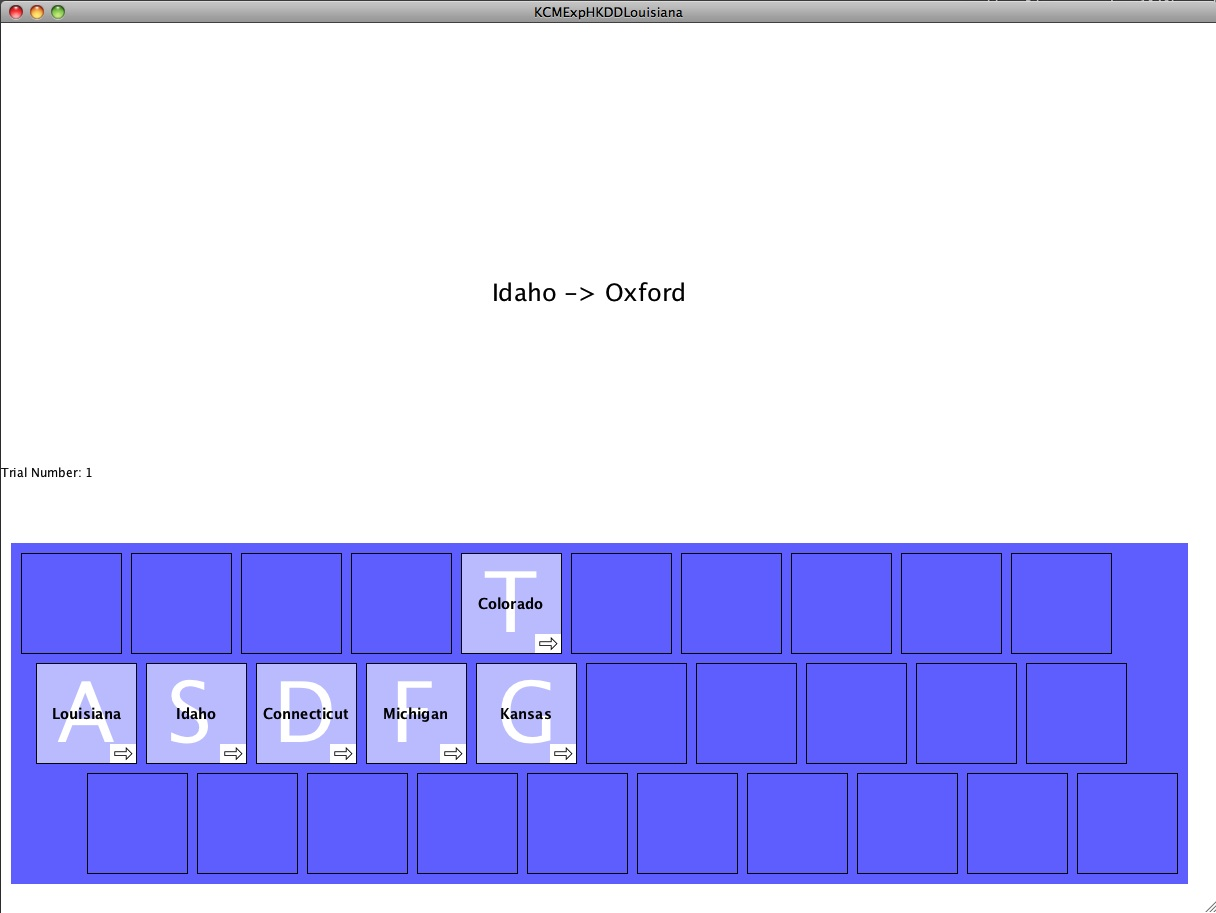
\includegraphics[width=\linewidth]{KCMIdahoOxford.jpg}
  \caption{In the study, described later in this paper, participants used a keyboard-card menu system, shown in the bottom half of the window, to select state-town pairs.  Seen here is actually the "root keyboard-card" of the menu system.  The small arrows in the corners of the keys indicate that there is a submenu associated with that key (a detail the participants did not have to rely on). When a user presses one of these keys, a child keyboard-card, such as the one seen in \autoref{fig:kcmoxfordzoom} appears. }
  \label{fig:kcmidahooxford}
\end{figure}

\begin{figure*} [t]
  \begin{center}
  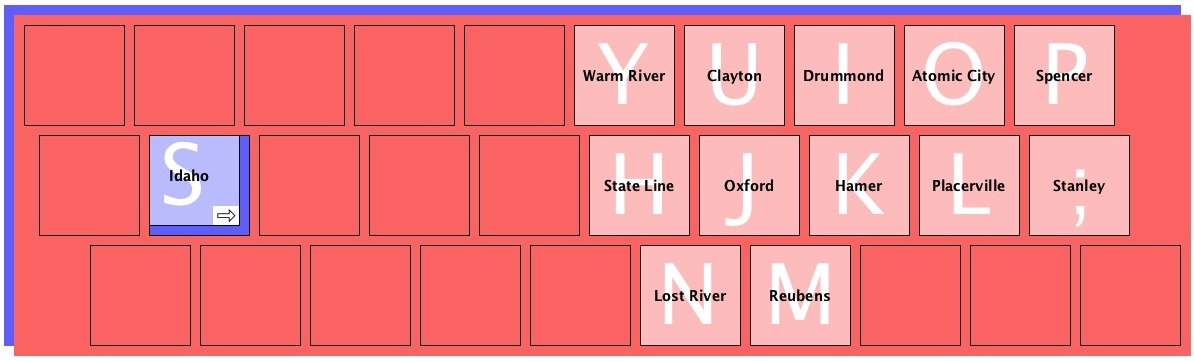
\includegraphics[width=\textwidth]{KCMOxfordZoom.jpg}
  \caption{The keyboard-card menu from \autoref{fig:kcmidahooxford} with the S key pressed.  Note how a hole has been ``punched out'' of the card.}
  \label{fig:kcmoxfordzoom}
  \end{center}
\end{figure*}

\begin{figure}
  \center
  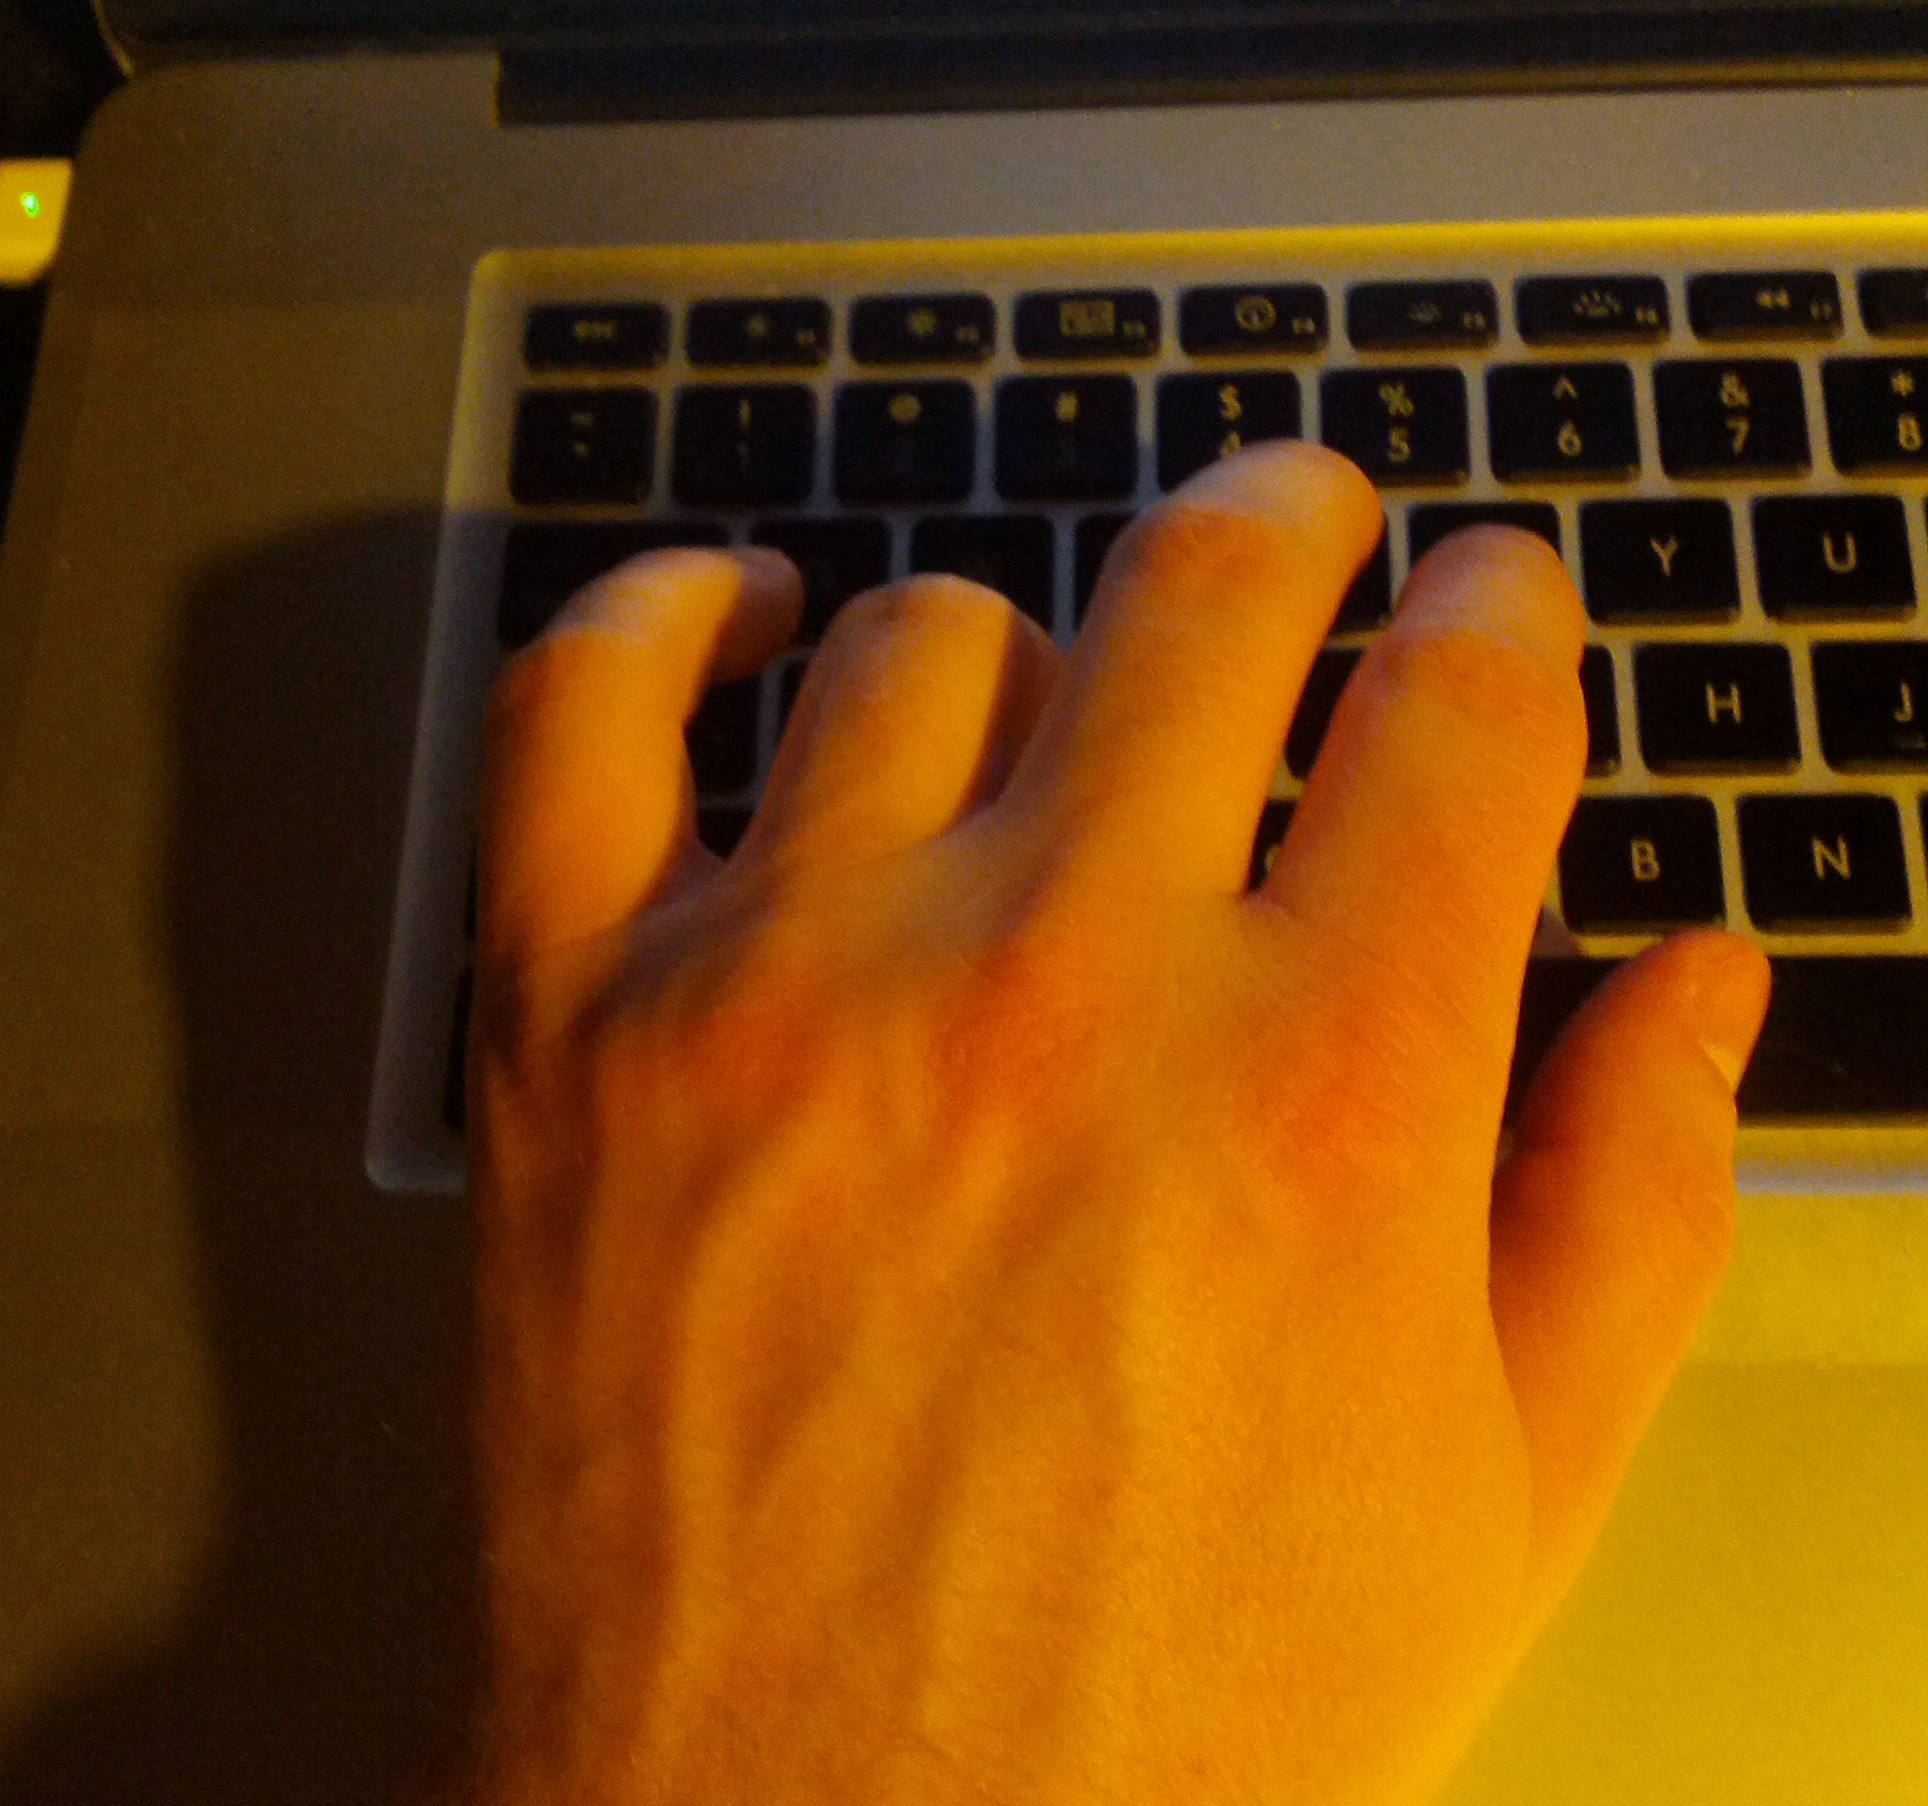
\includegraphics[width=\linewidth]{hand.jpg}
  \caption{Keyboard-card menus are intended to be used with a normal keyboard and monitor, not a touchscreen. The S key is pressed and held down to make \autoref{fig:kcmoxfordzoom} appear on the screen.  Whenever no fingers are held down, the menu appears as it does in the lower half of \autoref{fig:kcmidahooxford}, i.e. with a single ``keyboard-card'' instead of multiple ``stacked'' cards. }
  \label{fig:hand}
\end{figure}

Initially, when no keys are pressed, only the root card, with top-level menu items, is visible (as in the lower half of \autoref{fig:kcmidahooxford}).  Whenever a key corresponding to a submenu (rather than a leaf in the hierarchy) is pressed--\textit{and held down}--that submenu's keyboard-card is placed on top of the existing card(s), slightly offset to show the number of keyboard-cards below it (as in \autoref{fig:kcmoxfordzoom}, which would be displayed while the S key is held down).  %Releasing that key hides that keyboard-card again. 
When one releases the key, the corresponding submenu's keyboard-card disappears.
(Although the issue was ignored in our study, since no more than two cards, including the root card, were ``stacked'' at a time, releasing a key to hide a keyboard-card would most likely also just hide any cards on top of it, even if the keys associated with those cards were still pressed).  Holding down a key corresponding to a leaf in the menu hierarchy, in addition to performing whatever action is assigned, thickens the outline of the corresponding square on the fully-visible top card.

Because menu item selection is performed entirely from the keyboard, without the user having to move his hands, it can be very efficient.  In addition, simply by navigating the menu hierarchy, users end up practicing, and thereby learning, shortcuts needed to access menu items, and may actually stop needing the menu altogether. This idea of ``physical rehearsal''--teaching and reinforcing the physical act of using a shortcut during the process of navigating a menu hierarchy--can be found in work on gestures and ``marking menus'' by Kurtenbach and Buxton \cite{Kurtenback94, kurtenbach1993design}.   


% ==============================================
\subsubsection{Rolled-Chord Shortcuts}
\label{subsec:Rolled-Chord Shortcuts}
% ==============================================

The term ``rolled-chord'' comes from western classical music and refers to playing several notes together but initiating them at different times.  Here we use the term to refer to pressing multiple computer keys at the same time, but initiating the presses in a particular order.  However, while this term could be used to describe shortcuts involving special modifier keys (e.g. Ctrl-X, Alt-F4, Ctrl-Shift-S, etc.) we use the term to describe shortcuts where the modifier keys may in fact be letter keys.  (In applications where users need to type normal text, we assume that a separate mode would exist, as with the text editor \textit{vi} or its extension, \textit{Vim} \cite{Vim}).    For instance, one might press \textit{and hold} the F key, then press \textit{and hold} the D key, and, finally, press the J key to select some particular menu item.  In this paper, we consider only rolled-chord shortcuts using the letter keys plus the semicolon, comma, period, and forward slash keys on a QWERTY keyboard, since avoiding the use of special modifier keys has the advantage of reducing hand movement and therefore potentially increasing speed.

Rolled-chords are to be contrasted with ``standard'' chording in which the exact order of key presses does not matter because it is assumed that key presses are initiated simultaneously.  Standard chording may be used to achieve high speeds of data entry--on specialized keyboards, text entry speeds of up to 300 words per minute are possible \cite{Shneiderman10}.  While one would expect standard chording to be faster because no time is needed to ensure a particular ordering of key presses, ordering does provide more potential shortcuts and, in particular, more shortcuts that may be accessed without moving one's fingers off the home row of keys.  Furthermore, for sequences of shortcuts where the initial keys are identical, we can allow users to hold down those initial keys while pressing and releasing the final keys; for instance, over the course of entering the sequence of shortcuts ``F-J, F-K, F-J", the F key does not need to be released (we will use square brackets to indicate where keys are held down;  e.g. ``F-[J, K, J]'' indicates that the F key is held down while J, then K, then J, again, are pressed).

Rolled-chord shortcuts may also be contrasted with the use of short sequences of typed characters (e.g. ``: q ENTER'' is used to quit in \textit{vi}).  While such sequences remove limitations on the numbers of shortcuts that can be provided, rolled-chords
%, even using only two-key sequences, still provide hundreds of possible shortcuts (we suspect that having more than three, and possibly more than two, keys per shortcut would be impractical for many users) and, if absolutely needed, sequences of rolled-chords could still be treated as shortcuts.
still provide hundreds of possible shortcuts.  To see why, first consider only the shortcuts accessible by pressing two keys.  Some pairs of keys are clearly at least relatively awkward to press together.  For instance, pressing the W and the X keys together might best be accomplished by holding the W key with the ring finger while using either the middle or index finger to press the X key.  Of course this is not a terribly intuitive approach, since normally W and X are both pressed using the ring finger.  In addition, using the middle finger can be quite uncomfortable because of the tight connection between the middle and third fingers, and using the index finger may require a larger than normal amount of hand movement.  

We avoid these problems altogether if we consider just the two-key rolled-chord shortcuts invokable by pressing a key on one side of the keyboard followed by pressing a key on the other side of the keyboard (using first one hand and then the other; in the study described below we actually consider just a small subset of these).  Each side has 15 keys, so the total number of such available shortcuts is (2 sides) * (15 initial-keys/side) * (15 secondary-keys/initial-key) = 450.  For comparison, Microsoft Word for Mac 2011 \cite{MSOffice} contains approximately 230 leaves in its menu hierarchy, if one ignores the Font submenu which adds several hundred more (this is not to say that it would necessarily make sense to add rolled-chord shortcuts to any or all of the items in Microsoft Word's menu hierarchy, but, instead to suggest that many computer end-users and developers have already been exposed to menu hierarchies of such a scale).

We also hypothesize that rolled-chord shortcuts involving three (or perhaps even more) keys may be of practical value, despite being more complicated.  First, consider text editing in \textit{vi}, again, and the problem of moving the cursor around in the buffer.  Basic cursor movement is accomplished by pressing the H key to move left one character, the L key to move right one character, the J key to move down one line, and the K key to move up one line.  In addition, one can move around in larger increments, e.g. forwards or backwards a word, or to the beginning or end of a line, and up and down by paragraph or by page.  These larger increments require entirely different keys (e.g. W for forward a word), which we suspect means that many users just avoid pressing the faster movement keys (they may not fully recall what key to press and also wish to avoid accidentally deleting text).  

With an alternative text editor using rolled-chord shortcuts, one might use multiple keys in the left hand to select the speed of movement while still using H, J, K and L  in the right hand to select the direction.  For instance, one might press and hold F to go into a ``move'' mode and press J to move down a single line followed by L to move forward a character within that next line (recall that this would be ``F-[J, L]'' , i.e. the F key would not need to be released between J and L presses).  One could then add the D key to change the rate of movement to, say, 5 lines/characters per H/J/K/L press (i.e. ``F-[D-[... H/J/K/L key presses here ...]]'', so ``F-[D-[J, L]]'' would move the cursor down 5 lines and then over 5 characters).  One could, instead of D, add the S key to change the rate to, say, 20 lines/characters (so ``F-[S-[J, L]]" would move the cursor down 20 lines and then over 20 characters).  Or, instead of D or S, one could press A to move 80 lines/characters at a time.  

Because the F key is used in conjunction with the D, S, and A keys in this way, and the keys are designed to fit under the first, second, third and fourth finger (starting with the index finger), it is likely that
\begin{itemize}
\item the first two keys in the three-key sequences are at least relatively easy to press and hold down together, and
\item the intensity of the operation is roughly correlated with the center of gravity of the left hand relative to the keyboard and with its degree of rotation.  
\end{itemize}
Because of this correlation, and also because this use of three-key shortcuts could be generalized to applications, besides cursor movement in text editors, where varying degrees of intensity are called for (e.g. zooming and panning in maps, from the keyboard), this style of cursor movement might be considered more organized and intuitive than that of \textit{vi} and other editors.  The approach may also be used with other sets of keys (e.g. R, E, W and Q might be used in the alternative text editor to move the cursor while selecting text).

A second instance where having three-key rolled-chord shortcuts might be practical is simply to ``extend'' the number of keys (rather than intensifying the keys) that can be pressed after pressing the initial key.  Suppose, again, that the first key we press is F, but this time the items under the right-hand keys are codes for various medical procedures commonly associated with a hospital department.  If we have a list of up to 60 such procedure codes, we could extend the 15 right-hand keys using the D, S, and A keys, as in the text editing example above, while keeping them associated with the ``F''
department.

Third, three-key rolled-chord shortcuts may still be very fast, even relative to two-key rolled chord shortcuts.  This may be especially true when all three keys come from the center row of the keyboard (e.g. A-[F-[J]]) and so do not require finger joint extensions or contractions.

Rolled-chords also have several important advantages over simple key sequences.  First, in sequences like ``F-J, F-K, F-J" we may reduce the number of keystrokes needed, as explained above (``F, J, F, K, F, J'' vs. ``F-[J, K, J]'') .  Second, rolled-chord shortcuts enforce the rule, when assigning shortcuts to commands, that the keys pressed in a shortcut never use the same finger twice.  We suspect that following this rule increases speed; it also, as pointed out in \cite{PurdyJuly112012}, removes the possibility of accidentally entering a repeated letter sequence like ``F, F'' because of an operating system's key press repeater.  Third, when mistakes are made in selecting an initial key of a shortcut, no additional keystroke (e.g. "Backspace" or "Delete" key press) is needed to undo the mistake--the user simply releases the key.  This feature is especially important not only because it makes mistakes more preventable, but because it means that \textit{when the available shortcuts are displayed in a navigable hierarchy, as with keyboard-card menus, users can ``peek'' into submenus without having to press an additional key to back out again}.  We expect that this will help novice users considerably in exploring hierarchies and in searching for items that have non-obvious locations within the menu hierarchy.

Finally, one should not overlook the possibility of using forests of menu trees, and of using the shortcuts in one collection to move to another.  When all rolled-chord shortcuts are single-key, this would simply degenerate to simple key sequences.  Many applications might require a balance between one large tree and many small ones. 

% ==============================================
\subsection{Related Work}
% ==============================================

Encouraging shortcut use within graphical user interfaces is an active area of research.    A theoretical explanation of the problem of low levels of shortcut usage can be found in \textit{Paradox of the Active User} \cite{Carroll1987} which notes that people are biased towards using software to solve their immediate problems, rather than towards exploring what the software can do, and also generally prefer to use known solutions rather than new ones.  The severity of the problem has been empirically verified in \cite{Lane05}, and in trying to solve it researchers have gone so far as suggesting that the option to click on a dropdown menu item should be disabled when a keyboard shortcut is available \cite{Grossman07}.  

Our general approach--graphically supporting users in entering commands from the keyboard--has been taken before in a several alternate ways.  ``GEKA'' \cite{Hendy10} populates a list of command names and shortcuts, refining the list as users type, allowing a command line-like experience with a graphical user interface.  ``HotKeyCoach'' \cite{Krisler2008} uses a transparent popup window to inform and remind users of available (traditional) shortcut alternatives in a non-disruptive way as they work with an application.  ``Blur'' \cite{scarr2011dips} combines features seen in ``GEKA'' and ``HotKeyCoach'', notifying users when a command could be invoked by pressing escape and then typing ``hot commands'' (e.g. ``align left'') into a transparent popup window; it also provides lists of command recommendations.  ``ExposeHK'' shows users available (traditional) keyboard shortcuts when a user presses a modifier key; it replaces toolbar icons with printed shortcuts, expands all dropdown menus at once (with shortcuts printed next to the menu item name), and uses tooltips to show shortcuts for icons in a Microsoft \textit{Office 2007}-style ribbon \cite{malacria2013promoting}.

The line of work by Kurtenbach et al. on ``marking menus'' (which extend ``pie menus'' by allowing expert users to select items without looking at the menu) is in many ways parallel to ours, a major difference simply being the intended set of applications:  they assume a context in which users need some sort of pointing device most of the time (e.g. technical drawing), while we assume a context where most of the time users want to have both hands on the keyboard (e.g. text editing).  In particular, the design of keyboard-card menus follows three principles used in the design of marking menus  \cite{kurtenbach1993design}:  
\begin{itemize}
\item \textit{Self-revelation}:  interactively telling users what commands are available and what these commands do
\item \textit{Guidance}: showing users how to invoke commands during the process of self-revelation
\item \textit{Rehearsal}: guiding novice users through the same physical motions that an expert would use
\end{itemize}
A more recent alternative to marking menus, but still following these design principles, is ``OctoPocus'' \cite{Bau2008}.  Kurtenbach et al. also address the issue of providing large numbers of quickly accessible menu items in work on the ``HotBox'' \cite{Kurtenbach1999}.  

Work that most closely relates to ours may be explorations of interaction with multi-touch surfaces, since these provide a new opportunity for computer chording.  Relevant work includes ``Multi-finger Chorded Toolglass'' \cite{malik2007exploration}, ``Multi-Touch Menu'' \cite{Bailly2008}, ``Finger-count shortcuts'' \cite{Bailly2010}, ``Multi-touch Marking Menus'' \cite{Lepinski2010}, and, perhaps most significantly, ``Arpege'' \cite{bau2010arpege}. An advantage of using a multitouch surface is that thumb mobility may be exploited, as seen in \cite{Bailly2008} and \cite{malik2007exploration}. However, physical keyboards appear to be faster to type with than virtual keyboards on a multi-touch surface \cite{Varcholik2012657}, and using them in presenting chords does not create occlusion problems (involving the hands) which, as highlighted in \cite{bau2010arpege}, would likely make the presentation rolled chords much more complicated.

% =============================================================================
\subsection{Study Description}
% =============================================================================

% ==============================================
\subsubsection{Study Motivation}
% ==============================================

Keyboard-card menus are one of many possible ways to present rolled-chord shortcuts.  Using dropdown menus with menu items marked with letters, as in \autoref{fig:rcddmzoom}, as a baseline for comparison makes sense because of their advantages over keyboard-card menus and other types of menus, including that
\begin{itemize}
\item most existing applications already use dropdown menus, making the incorporation of rolled-chord shortcuts into the design of these applications somewhat more straightforward for software developers
\item users may feel more comfortable with them, since they are almost certainly more familiar with them
\item they do not hide submenu siblings (e.g. ``Massachusetts - F'' and ``Utah -T'' are still visible in \autoref{fig:rcddmzoom})
\item they are more compact (at least for relatively small hierarchies)
\end{itemize}

Reducing the advantage of compactness, screen resolutions have improved dramatically over the past decade \cite{BrowserDisplayStatistics} and secondary monitors are often available.  Some advantages of keyboard-card menus over dropdown menus are that
\begin{itemize}
\item since the size and shape of keyboard-card menus is relatively constant, the content being manipulated could never possibly be covered up by the menu
\item since dropdown menus typically have only a single row of items at the root level, they may allow for broader overall menu hierarchies, which have advantages over deep hierarchies \cite{Norman91}
\item the keyboard pattern makes using of the keyboard rather than the mouse the obvious choice
\end{itemize}

The last point may be the most important, though it is unclear how many users would decide to use the mouse rather than the keyboard if presented with labeled dropdown menus.  Finally, there is our \textit{experiment hypothesis}:

\begin{itemize}
\item new users are able to learn menu items' shortcuts faster
\end{itemize}

By this we mean both that the number of selections needed to memorize a shortcut is low and that the time to enter a shortcut that has not been memorized is low. 

\subsubsection{Initial Rationale for Experiment Hypothesis:} 

There are several reasons to think that keyboard-card menus might help users learn shortcuts faster.  First, although the size of each menu item's text is the same in both the keyboard-card and dropdown menu presentations, the character used to access the menu item is bigger, and therefore may be easier to read.  Second, the greater amount of space between menu items may also make misreading the character associated with a menu item more difficult.  Third, placing menu items in a two-dimensional array might help users exploit approximate information about locations because there are more characteristics that can be remembered.  For instance, given set of menu items, if these menu items are displayed in a one dimensional list, one might be able to remember that menu item ``A'' is above menu item ``B'', but, if the items are displayed in a two-dimensional array, one might be able to remember that ``A'' is above ``B'' \textit{and} one might be able to remember that ``A'' is to the left of ``B''. Fourth, with keyboard-card menus there is an alternate, and possibly faster, way to associate the key with the menu item, since the system could be used without looking at the character printed under the menu item.

After the experiment, we thought of a fifth, perhaps most likely, reason keyboard-card menus help users learn shortcuts faster.  This is given in our ``Discussion'' section, below.

% ==============================================
\subsubsection{Study Design}
% ==============================================
To see if the keyboard-card menu improves rolled-chord shortcut learnability relative to a dropdown menu presentation (i.e. relative to dropdown menus labeled as in \autoref{fig:rcddmzoom} that one navigates by pressing and holding keys), we performed a 20 participant (8 male) within-subjects comparison with adult self-described touch-typists as our participants, based loosely on \cite{Ahlstrom10} and \cite{Grossman07}. Participants were recruited through a mass email and word of mouth at a large state university in the United States.  After a 1 minute typing test (using the ``Space Cowboys'' test on typingtest.com), each participant performed up to 720 selection tasks (``trials'') over the course of at most 50 minutes, using one of the two menu systems, followed by half of a brief questionnaire.  The trials were then repeated, over the course of a second period of at most 50 minutes, using the second menu system with a second hierarchy of menu items, followed by the second half of the questionnaire.  Before each 50-minute period, participants performed 10 warm-up trials.  Participants were told that they could ask questions or take breaks at any point that would not count against the 50 minutes for each menu system, and participants were asked, at the 25-minute mark, if they would like to take a break.  Participants were also told that two thirds of the compensation would be prorated based on how many of the 1440 trials they completed.

In each trial, each participant was first prompted by text on the screen to press SPACEBAR, which started an invisible timer for the trial.  They were then presented with text of the form ``U.S. state -> small town'', e.g. ``Delaware -> Little Creek'' (see \autoref{fig:kcmidahooxford}); while the states were presumably recognizable by participants, the towns were unlikely to be recognized since they were selected from lists of the smallest towns in those states.  The trial ended when the town was correctly selected from the submenu labeled with the state's name, at which point the elapsed time was recorded and the participant was again prompted to press SPACEBAR to start the next trial.  The number of incorrect selections of town names during each trial was also recorded (usually this was zero).

Two non-overlapping hierarchies of states and towns were used.  Each consisted of 6 states and 72 towns, 12 from each state.  The states were assigned the A, S, D, F, G, and T keys and the towns were assigned the Y, U, I, O, P, H, J, K, L, semicolon, N, and M keys (as in \autoref{fig:kcmidahooxford}, \autoref{fig:kcmoxfordzoom}, and \autoref{fig:rcddmzoom}).  From each hierarchy, 14 towns, 2 or 3 from each state, were randomly selected for use in trials.  The 720 trials for each menu system were divided into 12 blocks of 60 trials, and the numbers of occurrences of each town in each block were 12, 12, 6, 6, 4, 4, 3, 3, 2, 2, 2, 2, 1, and 1, with the order varying randomly from block to block.  This organization of hierarchies and trials, and the Zipfian distribution used (``which has been shown to represent command use frequency in real applications''), was used in \cite{Grossman07}. 

While the same 14 towns for each hierarchy were used across participants, the numbers of occurrences were paired, randomly, with different towns for different participants (the pairing did not change across blocks for a given participant).  For instance, participants A and B would both see ``Delaware -> Little Creek'', but participant A might see it 6 times in every block while participant B might only see it 2 times in every block.

The numbers of participants were balanced between the four possibilities determined by whether the keyboard-card or dropdown menu was seen first and by which set of states and towns was used with which menu type.

The software for the experiment was run on a 2.8 GHz Intel Core 2 Duo MacBook Pro with Mac OS X Snow Leopard using Java 1.6.  However, participants viewed the software on an 18 inch, 1280 x 1024 pixel separate monitor (Dell Model No. 1800FP) and used a separate keyboard (Dell Model No. L100).  The experiment was performed in a faculty member's office on a university's campus. 


\begin{figure}
  \center
  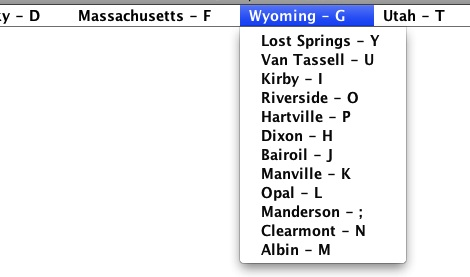
\includegraphics[width=\linewidth]{HKDDHartvilleZoom.jpg}
  \caption{Part of a dropdown menu, navigable by pressing and holding keys rather than with the mouse, used in the study; note the letters on each item.  Also note that the text is the same font and size as in the keyboard-card menus.}
  \label{fig:rcddmzoom}
\end{figure}




% =============================================================================
\subsection{Study Results}
% =============================================================================

The average selection times for the two different menu systems can be seen in \autoref{fig:averagetimes}.  Note that while outlier trials were removed (a trial was considered an outlier if its time was greater than 3*(Q3-Q1)+Q3, where Q1 and Q3 were the first and third quartile values; 0.55\% of trials were considered outliers), average times for participants who did not complete all 1440 trials were left in.  Averaged trial completion times for each block  are only complete for all participants and menu types in blocks 1-8.  One participant was only able to complete trials in blocks 1-8 for both menu types.  Two other  participants were only able to complete trials in blocks 1-10 using the dropdown menus, but were able to complete trials in all blocks using the keyboard-card menus.  The remaining 17 participants were able to complete trials in all blocks.

\begin{figure}
  \center
  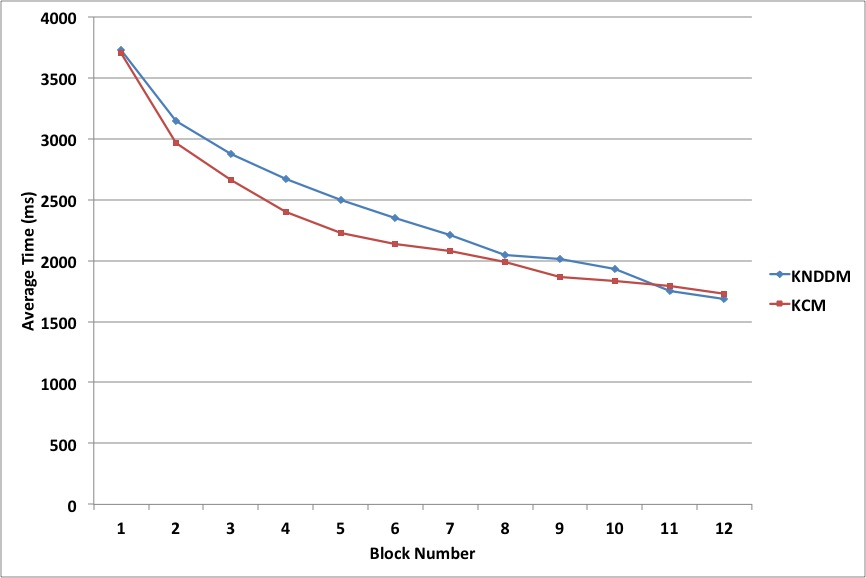
\includegraphics[width=\linewidth]{AverageTimes.jpg}
  \caption{Average trial completion times, in milliseconds, for the keyboard-navigated dropdown menus and keyboard-card menus in the study.  Note that data is only complete for blocks 1-8}
  \label{fig:averagetimes}
\end{figure}

To analyze this data we fit quadratic equations, as first approximations, to the completion time data for each participant (with trial number as the independent variable and completion time as the dependent variable), leaving out times for trials where any participant was missing data (due either to an outlier completion time or to not being able to complete all trials), the result of which was complete data for 323 trials over blocks 1-8; the averages of the times for these individual trials are shown in \autoref{fig:AverageIndividualTrialsComplete}.  Paired t-tests on the coefficients of the fitted quadratics showed statistically significant (p = 0.0458) differences between the average second-order coefficients for keyboard-card and dropdown menus (i.e. there were statistically significant differences in the ``curviness'' of the data for the keyboard-card and dropdown menus).  In addition, we performed a repeated measures ANOVA on the average completion times for blocks 1-7 (where all participants completed all trials), which showed statistically significant differences between the two menu types (p = .044) as well as between the blocks (p < .001).


\begin{figure}
  \center
  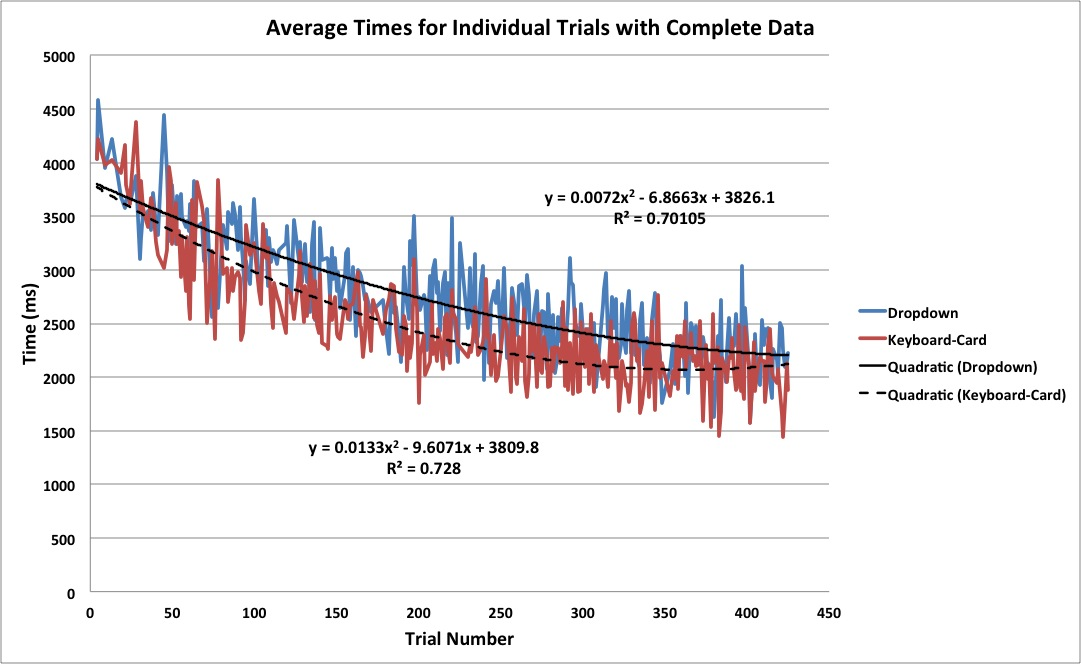
\includegraphics[width=\linewidth]{AverageIndividualTrialsComplete.jpg}
  \caption{Average times across participants at individual trial numbers where data is complete.  These individual trials come from blocks 1-8.  Also included are quadratic curves fit to the data.} 
  \label{fig:AverageIndividualTrialsComplete} 
\end{figure}

Average error rates for each trial and menu type are shown \autoref{fig:errorrates}.  Overall error rates across blocks 1-7 for the dropdown menus and keyboard-card menus were 10.4\% and 8.4\% respectively, where errors were defined as the incorrect selection of a leaf in the menu hierarchy and the error rate for a block was calculated as $e/(e+t)$ where $e=$ the number of errors in the block's non-outlier trials and $t=$ the number of non-outlier trials in the block.  This difference was not statistically significant.  However, t-tests on the data for the 5th, 9th and 10th block differences did show statistical significance (p-values were .032, .008, and .049 respectively; note that 9th and 10th blocks exclude data for one participant).  Though a repeated measures ANOVA on the error rates for blocks 1-7 also failed to show statistical significance, fitting quadratics to the error rates for each participant at each block where data was available, and then performing t-tests on the coefficients \textit{nearly} showed statistical significance at the 5\% level for the quadratic and linear coefficients (p-values were .0544 and .0624 respectively)

Several interesting correlations can also be seen in the overall (i.e. across blocks) data for each participant.  Error rates for dropdown menus were correlated ($R=$0.718) with the error rates for keyboard-card menus and overall average times for dropdown menus were correlated ($R=$0.911) with overall average times for keyboard-card menus.  However, error rates and average times were negatively correlated for both dropdown menus and keyboard-card menus ($R=$ -0.510 and -0.479, respectively), so it appears that some participants chose to concentrate more on being accurate, at the expense of speed, and some chose to do the opposite.

In addition, the difference between the error rates for dropdown and keyboard-card menus was positively correlated with the error rate for dropdown menus (see \autoref{fig:errorratedifferences}) and the difference between the average times for keyboard-card and dropdown menus was positively correlated with the average times for dropdown menus (see \autoref{fig:timedifferences}).  In other words, participants whose error rates were higher made even more mistakes when using the dropdown menus, and participants whose average times were slow were even slower  when using dropdown menus.

\begin{figure}
  \center
  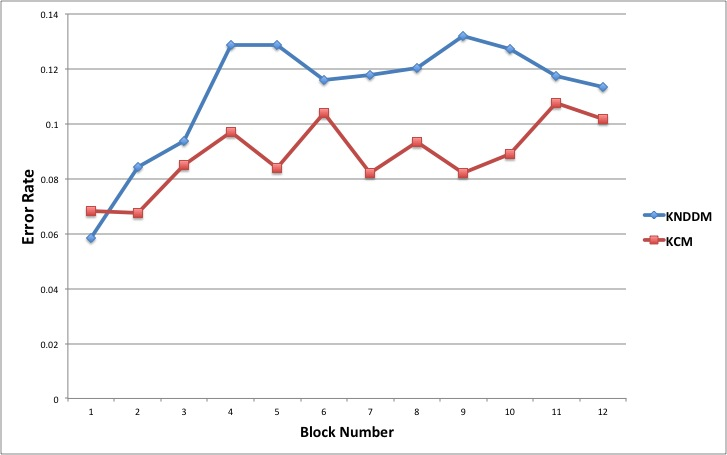
\includegraphics[width=\linewidth]{ErrorDataFixed.jpg}
  \caption{Error rates for the keyboard-navigated dropdown menus and keyboard-card menus in the study.  Note that data is only complete for blocks 1-8.}
  \label{fig:errorrates}
\end{figure}

\begin{figure}
  \center
  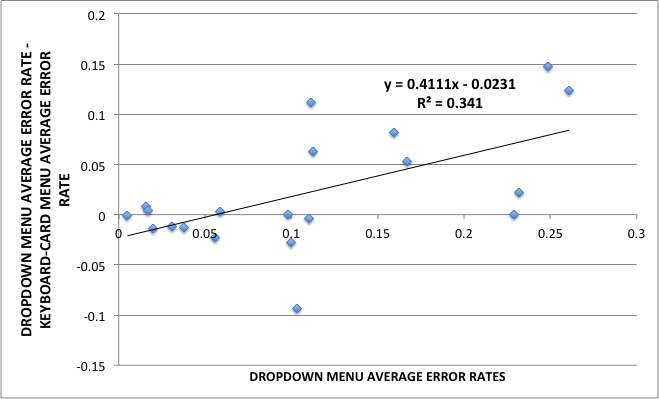
\includegraphics[width=\linewidth]{ErrorRateDifferences.jpg}
  \caption{The differences between the overall average error rates for dropdown menus and keyboard-card menus, for each participant, plotted against the error rate for dropdown menus.}
  \label{fig:errorratedifferences}
\end{figure}

\begin{figure}
  \center
  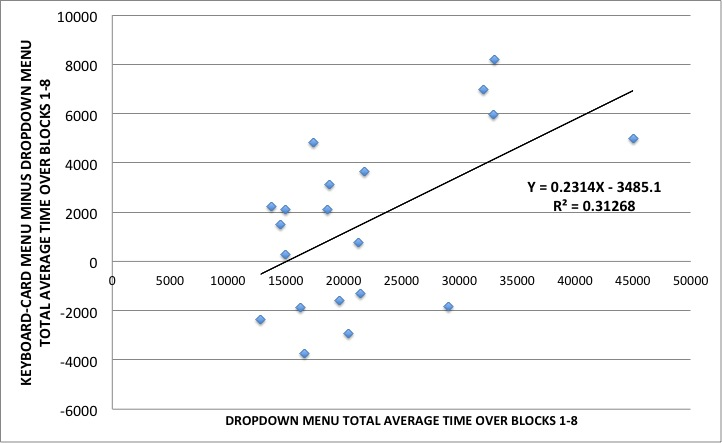
\includegraphics[width=\linewidth]{OverallAverageTimeDifferences.jpg}
  \caption{The differences between the overall average times for dropdown menus and keyboard-card menus, for each participant, plotted against the time for dropdown menus.}
  \label{fig:timedifferences}
\end{figure}

Results from the questionnaire can be seen in the table, where
\begin{itemize}
\item Q1=``How quickly do you feel you were able to become familiar with the menu item locations over the course of performing the trials?''
\item Q2=``At the beginning of the set of trials for this menu system, how quickly do you feel you were able to select menu items?'', and
\item Q3=``At the end of the set of trials for this menu system, how quickly do you feel you were able to select menu items?''
\end{itemize}
Ratings were given on a scale from 0=``Very Slowly'' to 9=``Very Quickly''.  Though the results of these ratings were favorable for keyboard-card menus, t-tests did not reveal statistically significant differences between the average ratings (p-values given in the table). These results were not correlated with typing speed.

\begin{table}[h]
  \centering
  \begin{tabularx}{\linewidth}{ |X|X|X|X|X|X| }
  \hline
   & \bf{KCM Ave.} & \bf{KCM Std. Dev.} & \bf{DDM Ave.} & \bf{DDM Std. Dev.} & \bf{P-values} \\
  \hline
  \bf{Q1}  & 6.0  & 1.5  & 4.8 & 2.4 & .165  \\
  \hline
  \bf{Q2}  & 3.0  & 1.8  & 2.2 & 1.6 & .119  \\
  \hline
  \bf{Q3}  & 7.3  & 1.3  & 6.7 & 2.1 & .525  \\
  \hline
  \end{tabularx}  \caption{Questionnaire Results.}
  \label{tab:myfirsttable}
\end{table}

In addition, two open-ended questions were given in the questionnaire:
\begin{itemize}
\item Q4 = ``For this menu system, did you notice anything that made selecting items difficult?  If so, please list and explain.''
\item Q5 = ``Having used both menu systems, which do you prefer? Why?'' 
\end{itemize}
Q4 was repeated twice, once in the first half of the questionnaire (taken immediately after using first menu type) and once in the second half at the end of the session.  Q5 was the last question in the second half of the questionnaire.

For Q5, 12 of the 20 participants wrote that they preferred the keyboard-card menu, while 8 wrote they preferred the dropdown menus (though with one of the 8, the explanation appeared to give an argument in favor of the keyboard-card menus, so a mistake may have been made in that case which would make the numbers 13 and 7).  Explanations for the preference towards the keyboard-card menus included:
\begin{itemize}
\item ``I seemed to pick up the shortcuts faster.  It felt easier to use''
\item ``There was more visual association in the second''
\item ``...it gave me a visual of where I needed to type with the keyboard image on the screen.  I thought I learned the second menu faster.''
\item ``I felt I got accustomed to it more easily [and] quicker.  I believe I finished the 720 trials in the first faster.''
\item ``...it was easier for me to understand it''
\item ``the layout is more intuitive and it's easier on the eyes.''
\item ``...easier to become familiar with choices''
\item ``Modeling where to press on the keyboard was helpful, as were the color shifts.  It was also easier on the eyes (looking at it was less of a hassle).''
\end{itemize}

On the other hand, some of the explanations of preference from participants favoring the dropdown menus included:
\begin{itemize}
\item ``I feel like I was faster with the second procedure.  However I believe I made more mistakes along the way.''
\item ``The [keyboard-card menu] might be better for those that use the `vulture' method of typing as it shows where the key is.  The extra space in this layout just makes it take longer to read  the flashing colors are distracting once the combinations are memorized.''
\item ``although it's slow starting out, I memorized the keys faster, plus the first one made me feel a little sick D: ''
\item ``more familiar with ``dropdown'' menu''
\item ``I like the first menu system because it takes up significantly less space, and it has more flexibility.''
\item ``because then I didn't try to look and check each time.''
\item ``I was able to catch on quicker''
\end{itemize}

Answers to Q4 after using the keyboard-card menu included:
\begin{itemize}
\item ``Had trouble w/ Kentucky --> might help to alphabetize the key strokes, e.g. `D' for `Delaware'
\item ``I was thrown off that Indiana was `A' rather than `I', etc.  Also, it was kind of hard to read the words printed over the letters on the screen."
\item ``I didn't like the change of colors from blue to red --> hard to get used to''
\item ``At the beginning the color changes were distracting toward my goal, but the visual layout soon became helpful.''
\item ``The visual distance between the prompt + the on-screen keyboard''
\item ``Keys close to each other''
\item ``I couldn't remember where half the towns were.  Seemed to take a long time to locate some cities.''
\item ``I still wanted to sometimes hit the key that corresponded to the letter of the word.''
\item ``Same first letter for states would have made it easier''
\item ``The background letter images made it harder to read the words.''
\item ``That the names on the left disappeared so if you made the wrong selection you had to depress the key to continue scanning the list.''
\item ``Had to read from left to right at first."
\item ``The words sometimes mix with the letter in the key''
\item ``Confusing at first''
\item ``expanding beyond the home row key set, such as using the key `T'.''
\item ``having to move up for colorado and right for kansas threw me off a little. fingers had gotten used to staying still''
\end{itemize}

Answers to Q4 after using the dropdown menu included:
\begin{itemize}
\item ``Despite the number of trials, it took me forever to learn which letter corresponded to which state (some in the middle I didn't learn).  Were menu items ordered in any way? I didn't really pick up on it if they were.  Holding down one key and then pressing the other could be awkward when the keys were close together.  Maybe the commonly-used items could have moved to the top of each menu to make it easier.  Tasks were rapid-fire--I thought I was trying to go a little too fast sometimes''
\item ``With the state/city combination I was tempted to do the combination of keys that corresponded with the first letters of the word.  ex Kentucky -> Fairfield I wanted to do K - F.''
\item ``There were way to many choices''
\item ``beginning letter of state [and] beginning letter of city''
\item ``I was inclined to associate letters with the names of the places (L - little creek) so the lack of matching made it more difficult.  Also, when I had to shift from the standard typing position (G/H for instance) my response time slowed''
\item ``It's much more difficult to read off a dropdown list than with the keyboard layout.  Also, the dropdown list is not in alphabetical order, which oftentimes mislead me to the wrong answer.''
\item ``One thing that I found difficult was when the letters of two options were close together on the menu.  I kept on switching them around in my head and sometimes forgot which was which.'' 
\item ``I felt like my eyes were doing more work looking around the screen than [with the keyboard-card] trials.  Also, having towns on keys which didn't correspond w/ their first letter made it difficult at first.''
\item ``My first instinct would be to hit `L' for Louisiana rather than `A', `C' for Connecticut rather than `D', etc.  Also, the cities under each state's menu were not actually cities in these states, so it was hard to remember their names.''
\item ``It was hard to keep track of the Connecticut/Canaan and Connecticut/Cornwall difference.  It was very difficult locating the names on the dropdown lists.''
\item ``They weren't in alphabetical order''
\item ``At the start, I had to scan the list to find out which key belonged to which city.  That lost me some time"
\item ``The place to look for second menus keep changing and sometimes I would even have to spend time looking for where the menu is.''
\item ``Some menus were in alphabetical order \& others weren't.  Also as one key had to be held down this slowed me as I became more familiar \& memorized combos because sometimes they weren't recognized when typed too fast if my finger didn't stay on the 1st key''
\item ``Utah -Scofield were right next to one another [using the T and U keys], which made it awkward.  Also, there was no alphabetic order to the menu, so it took a long time to find unfamiliar items.''
\end{itemize}

% =============================================================================
\subsection{Discussion}
% =============================================================================

The selection time data supports the hypothesis that the keyboard-card menu's presentation makes rolled-chord shortcuts easier to learn than does the dropdown menu's presentation.  We further hypothesize, first, that the eventual convergence of the two curves in \autoref{fig:averagetimes} means that by the 12th block users had (mostly) memorized the 14 shortcuts (and so were not using either presentation), and second, that the initial divergence of the two curves indicates that the keyboard-card menu's presentation mostly helped users in finding and recalling shortcuts they had seen but not fully memorized.  

Although in \autoref{fig:averagetimes} the separation between the curves appears to be small, it may be exaggerated considerably in more realistic applications by two factors.  First, the period in which users have seen menu items but have not yet memorized their locations (i.e. the middle section of \autoref{fig:averagetimes}) may be extended over a greater period of time (e.g. hours or days, rather than tens of minutes) affecting the number of menu selections needed for memorization.  Second, the effect of errors on the average selection times would likely be much greater, since only the time needed to make an error, recognize it, and make a correct selection is included in the \autoref{fig:averagetimes} data;  in realistic applications, the time to undo an error would also have to be included.

The negative correlation seen between error rates and average times shows users making a tradeoff between speed and accuracy.  However, the data seen in \autoref{fig:errorratedifferences} and \autoref{fig:timedifferences} suggests that use of a keyboard-card menu instead of a dropdown menu can help both users who prefer speed to accuracy and users who prefer accuracy to speed.

After performing the study, we have come up with a relatively simple explanation for the differences between both the average time curves \textit{and} the error rate curves, not among the four given in the ``Study Motivation" section above:  keyboard-card menus make it easier for users to check their knowledge of the shortcuts.  For instance, suppose a user has gained only an intermediate level of experience with the shortcuts and, therefore, wants to check that the shortcut ``D-[L]'' is the one he wants to use.  To check this using the dropdown menu system \textit{without actually invoking the shortcut}, he would have to press and hold the D key and then visually scan through the list of items that appear until he either sees the L key in the list or the menu item itself.  In contrast, after pressing the D key using the keyboard-card system, he can move his gaze much more directly to the position of the menu item associated with the L key because he knows where the L key is within the keyboard layout.

From the written responses to the questionnaire, several issues emerged as significant.  First, the menu items were not organized either alphabetically or by item frequency.  Second, how far users had to move their fingers to invoke a shortcut (e.g. the U key vs. the J key) mattered to them.   Third, users' normal expectation is that the shortcut key used will be the same as the first letter of the menu item.  Finally, some users found the bright flashing colors bothersome.  How much these issues actually slowed users down, and how much they affect users' overall feelings about the shortcuts, remain to be investigated.  However, they may be used as an initial set of heuristics in future keyboard-card menu applications (e.g. given a choice between associating a menu item with the U key or the J key, pick the J key).

% =============================================================================
\subsubsection{Future Work}
% =============================================================================

Many issues surrounding keyboard-card menus remain unexplored.  Perhaps the most important next step is to test the menu system in an actual application; one such application under consideration is interactive theorem proving with the Coq Proof Assistant\cite{Coq}, since its use involves manipulation of a wide variety mathematical notations using a large set of commands.

Other questions that may be addressed (many of which arise from the results of the study discussed in this paper) include:
\begin{itemize}
\item Does the menu actually encourage first time users of a system to use the shortcuts? 
\item What happens when icons instead of, or in addition to, labels are used?
\item What is the best way to map a hierarchy to the menu?
\item What happens when three finger shortcuts are used?  
\item Can keyboard-card menus' presentation be effective with other sorts of shortcuts (e.g. simple key sequences)? 
\item What sorts of color schemes should be used?  Should bright colors be completely avoided because they seem to bother some people?   Should each card have its own color/texture to make it easier to tell where one is in the hierarchy?  (In the study, all sub-cards in the second level were red).
\item How much of a difference does it make to assign a menu item to a key that matches the first letter of the menu item (e.g. assigning the ``Idaho'' submenu to the I key)?  And if one were to do so as much as possible, would inconsistencies caused having two items with the same initial letter make the error rate go up?  Would removing the large letters from the keys in the keyboard-card menu help reduce confusion?
\item Would using dropdown menus alphabetized by shortcut character, with or without extra ``inactive'' locations, make up the difference in times seen between the two menu types in the study? Would alphabetizing by menu item name (e.g. placing ``Atomic City'' ahead of ``Clayton'') in the menus have made any difference?
\item What can we do to prevent users from missing shortcut invocations because they type too fast?  For instance, would keeping a submenu key ``active'' for a few milliseconds after it is released fix the problem?  Can we try to guess the intended shortcut (e.g. can we sometimes assume that ``F, J'' was meant to be ``F-[J]'' if ``J'' by itself is not a valid shortcut)?
\item How effective are these menus for users who do not touch type?
\item How much of the difference does using keys other than A, S, D, F, J, K, L, and semicolon make in expert speed, learnability, accuracy, etc.? 
\end{itemize}


% =============================================================================
\subsection{Conclusion}
% =============================================================================

While selecting from a large set of menu items in an efficient manner is certainly possible, expecting users to learn how to do so using traditional shortcuts displayed in dropdown menus is often unrealistic.  In order to open up new realms of computer applications to a wider range of users (college students typing of mathematics at the computer, for instance), we are rethinking shortcuts and, in particular, how to present them.  We have developed keyboard-card menus, and have tested them against dropdown menus as a way of presenting how to enter shortcuts, using rolled-chords as our shortcut choice in the experiment.  Our data shows that keyboard-card menus, taking advantage of increasing amounts of available screen space with their keyboard-shaped presentation, can be more effective than a presentation based on dropdown menus as a method for presenting large numbers of shortcuts in an easy-to-learn way. 

% =============================================================================
\subsection{Acknowledgements}
% =============================================================================

We would like to thank our participants for their time and effort.  This research was supported by NSF award CCF-1250306.



\section{Keyboard-Card Menus + Syntax Tree Highlighting:  A Case Study with a Subset of Coq}

Here I briefly present a prototype structure editing\footnote{In general, this means editing with an awareness of document validity restrictions, in contrast to systems that work by entering text character by character--many existing systems might be viewed as hybrids.  Coq, because of its tactic system for building proofs, could itself be considered a structure editor.} system.  The system uses keyboard-card menus to move segments of highlighting within the buffer around, in accordance with the underlying syntax tree.

There are several major benefits of this approach.  First, particularly for systems like Coq that involve complex nesting of (often computer-generated, poorly formatted) code, the approach may help users understand the structure of the text, without having to leave the editing environment.  Second, it prevents users from writing many classes of ill-formatted code in a way that may be especially useful to novice users unfamiliar with the rules of the language.  Third, it allows boilerplate code to be easily inserted from templates, reducing the number of necessary key strokes.  Finally, it comes with the learnability advantages of Keyboard-Card menus, as discussed in the previous section.

Perhaps the best way to understand this system is through an example.  In \autoref{fig:pl0} we see the initial state of the system.  The dark green text represents the currently selected node.  In general, text between ``(*'' and ''*)" is comment text, and throughout this example is being used to show ``placeholder'' text that either must or could be filled in.  In \autoref{fig:pl0}, this placeholder text indicates that a propositional variable is required.  The keyboard-card displayed in the bottom half of the window is already set up so that a propositional variable may be typed in.  (In future versions of the keyboard-card menu system, keyboard-cards with different, and possibly larger, sets of keys may be supported so that, for instance, the slash key does not need to be used for backspace).    

\begin{figure}[H]
  \center
  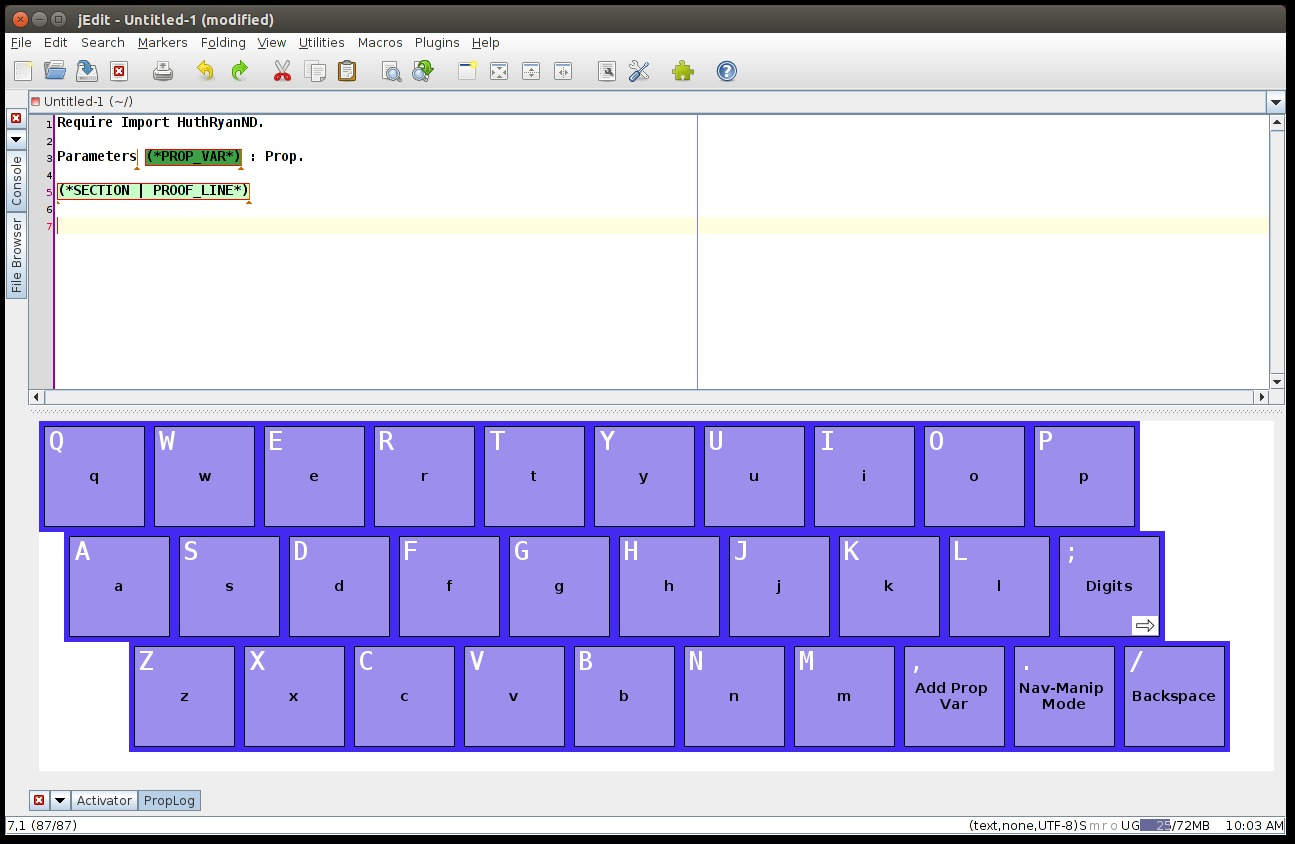
\includegraphics[width=\linewidth]{pl0.jpg}
  \caption{}
  \label{fig:pl0}
\end{figure}

\autoref{fig:pl1} shows the system after the A key has been pressed but before it has been released (hence the graying out of key labels).  Once the A key has been released, other keys can in fact be pressed so as to enter multi-character identifiers.

\begin{figure}[H]
  \center
  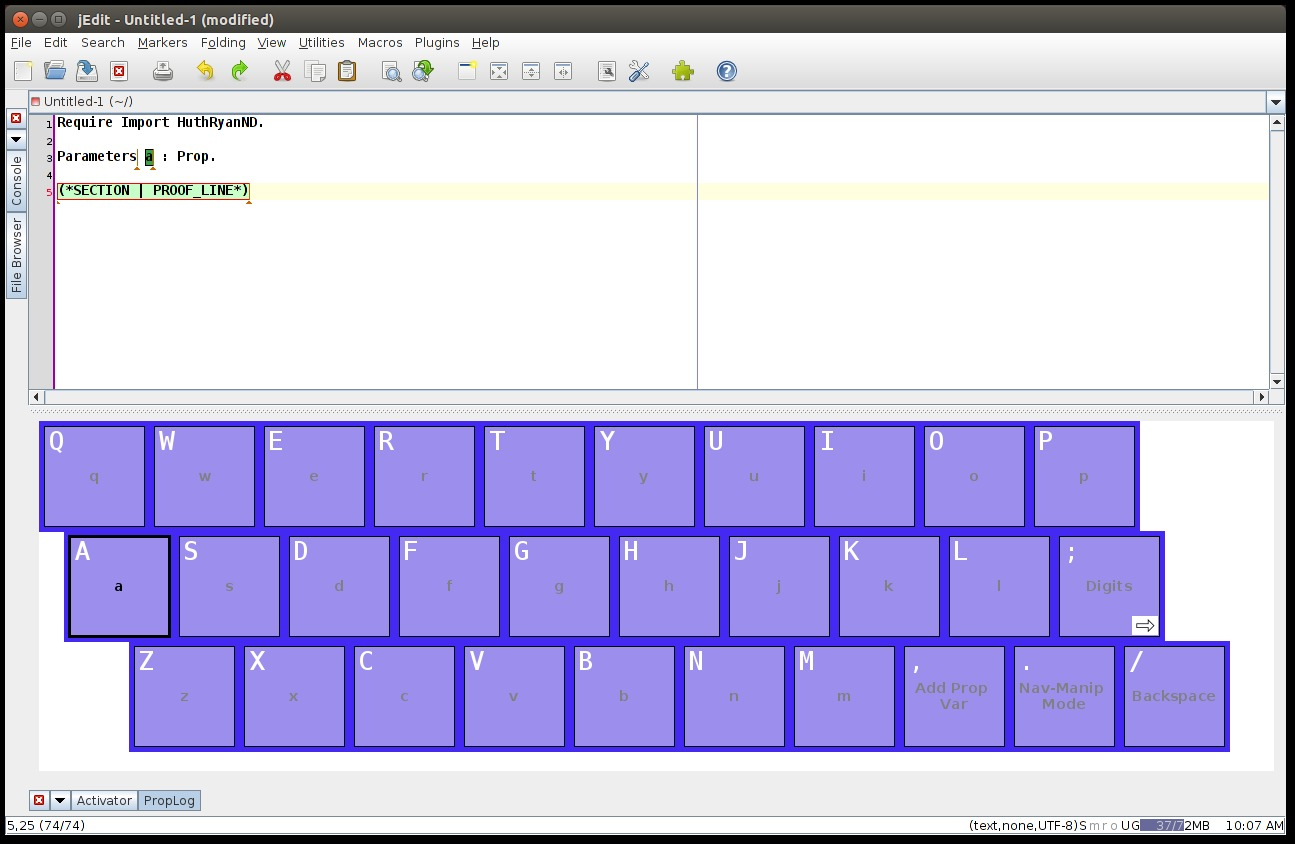
\includegraphics[width=\linewidth]{pl1.jpg}
  \caption{}
  \label{fig:pl1}
\end{figure}

\autoref{fig:pl2} shows the result of releasing the A key and pressing the period/``Navigate and Manipulate Mode'' key.  This has the effect of changing the current keyboard-card menu card tree so that the Nav-Manip root card is displayed and active. 

\begin{figure}[H]
  \center
  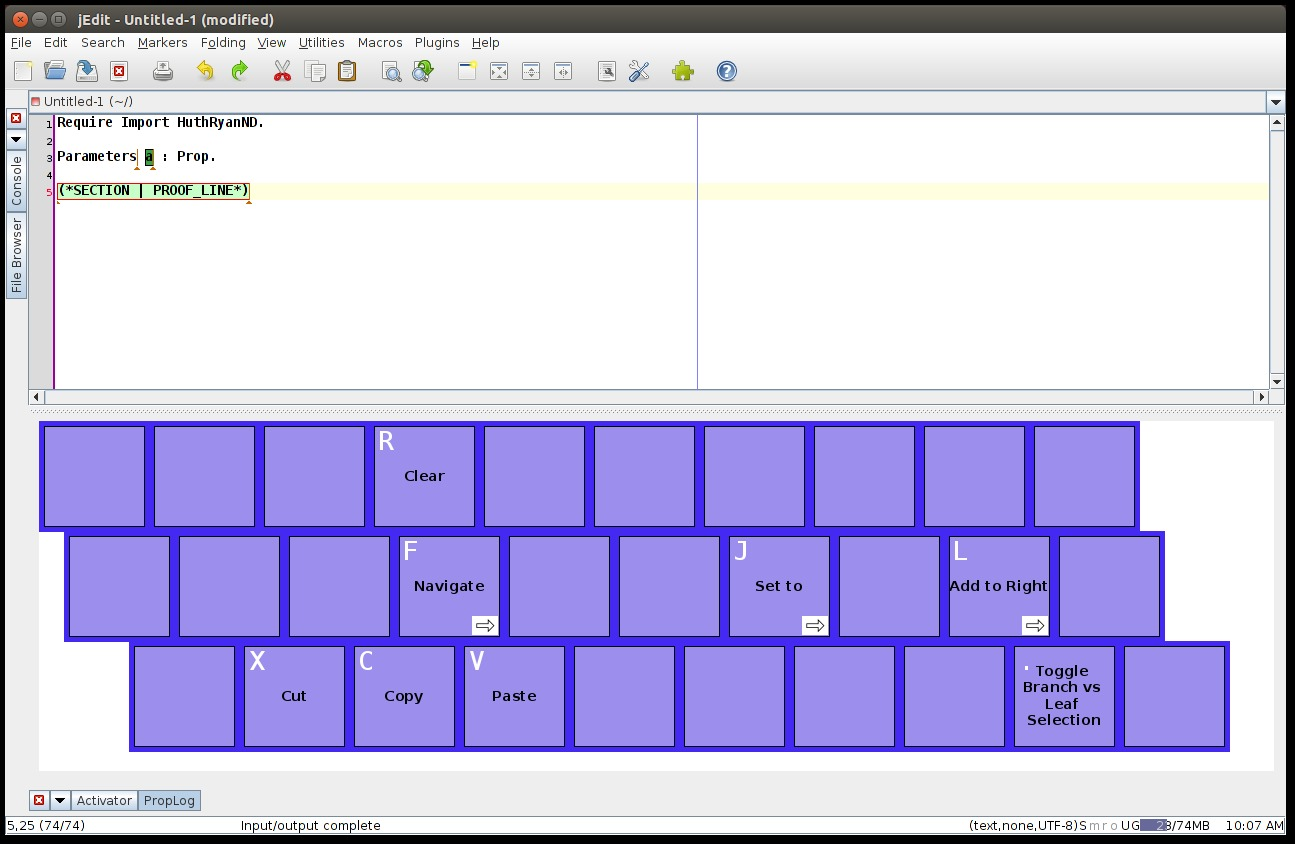
\includegraphics[width=\linewidth]{pl2.jpg}
  \caption{}
  \label{fig:pl2}
\end{figure}

In \autoref{fig:pl3} we see using the navigation submenu to move to the next leaf in the tree.  This is actually a placeholder for an optional list of space-separated propositional variables.  Placeholders for optional text only appear in full when they are selected, and are otherwise marked with a small triangle below the line of text and a vertical line within the line of text.

\begin{figure}[H]
  \center
  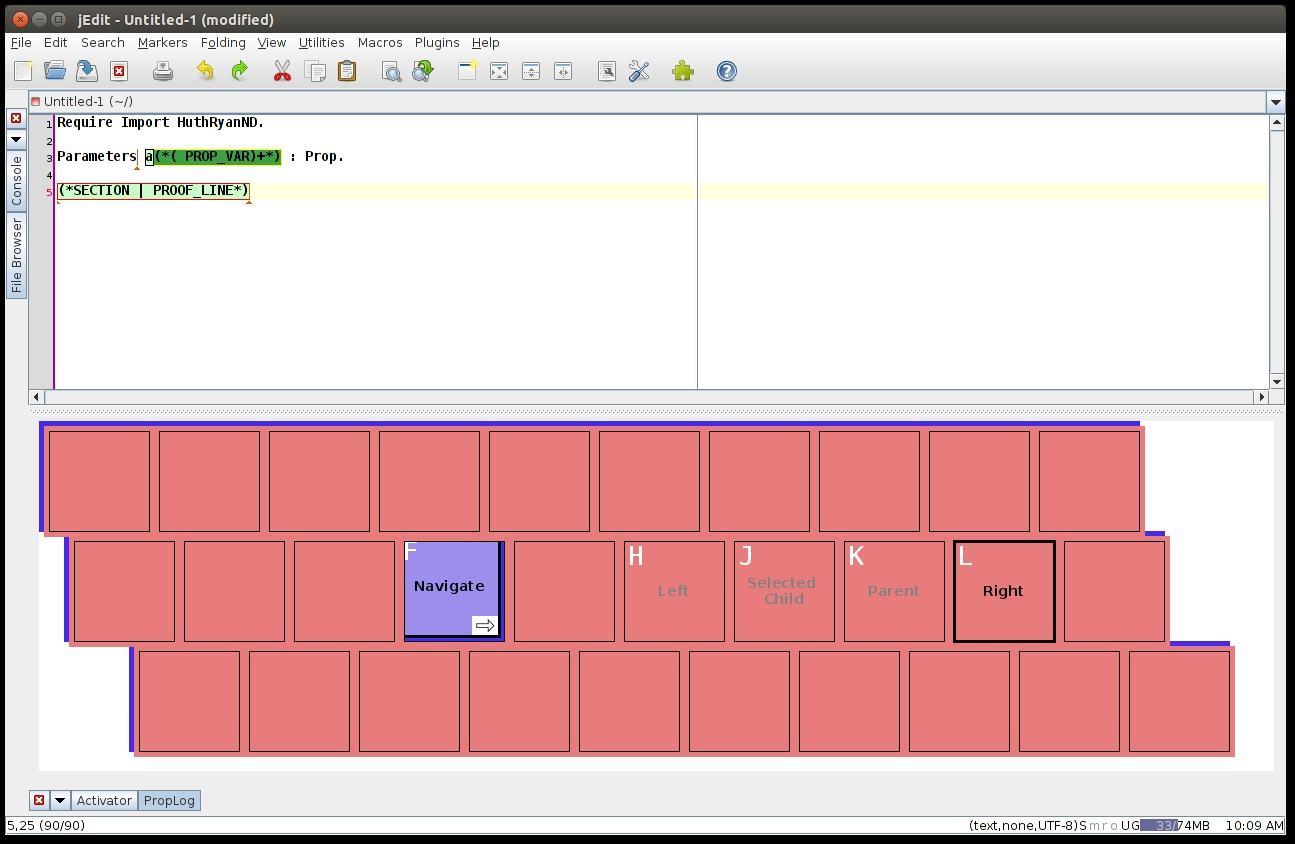
\includegraphics[width=\linewidth]{pl3.jpg}
  \caption{}
  \label{fig:pl3}
\end{figure}

\autoref{fig:pl4} shows the ``Set to'' submenu, after the user has moved right two more positions to where ``Sections'' and ``Proof Lines'' can be inserted.  In future versions of the editor, the other items in the submenu may be grayed out, but at present their selection has no effect.

\begin{figure}[H]
  \center
  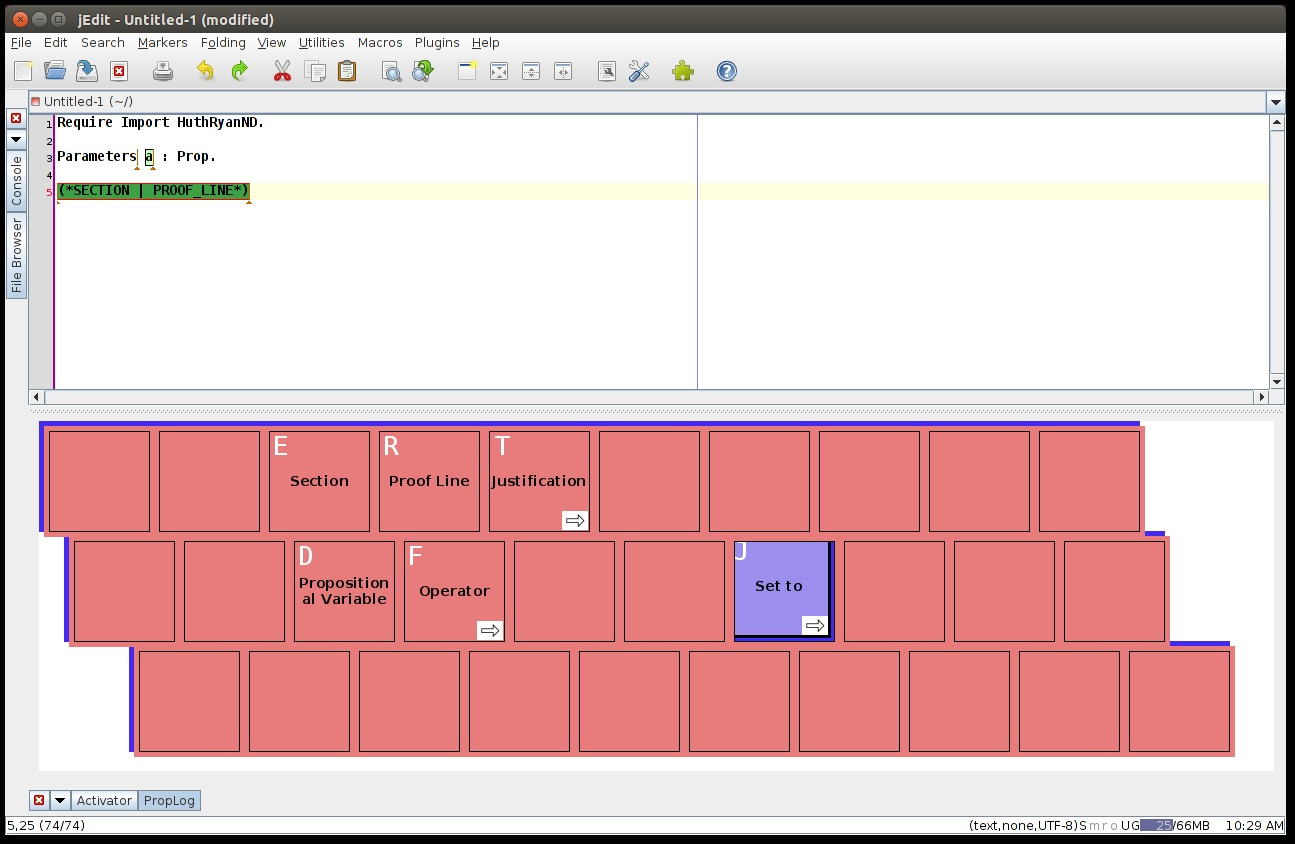
\includegraphics[width=\linewidth]{pl4.jpg}
  \caption{}
  \label{fig:pl4}
\end{figure}

Selecting ``Proof Line'', as in \autoref{fig:pl5} has the effect of inserting a line starting with ``Fact..''.  The ``Line Identifier'' node is selected, and can be edited using a keyboard-card tree similar to that seen in \autoref{fig:pl0}.  The user switches to this keyboard-card tree by pressing the ``Set to'' submenu key while the Line Identifier placeholder is selected---in this case, the submenu key behaves like a leaf key.

\begin{figure}[H]
  \center
  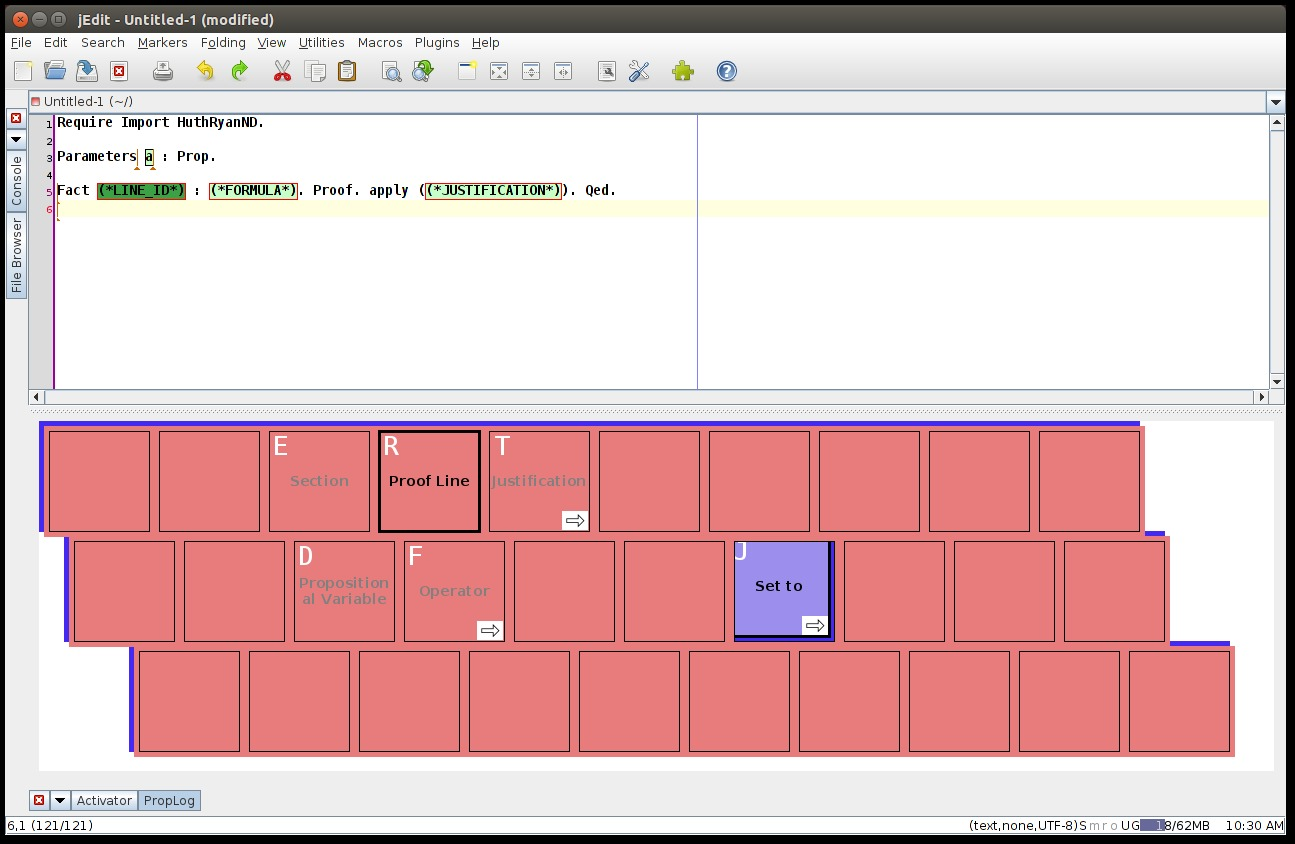
\includegraphics[width=\linewidth]{pl5.jpg}
  \caption{}
  \label{fig:pl5}
\end{figure}

After switching back to Nav-Manip mode and moving to the formula placeholder, the ``\textbackslash/'' (OR) operator may be inserted along with two formula placeholders.  This is accomplished by displaying the ``Operator'' submenu from the ``Set to'' submenu (so three fingers are involved).

\begin{figure}[H]
  \center
  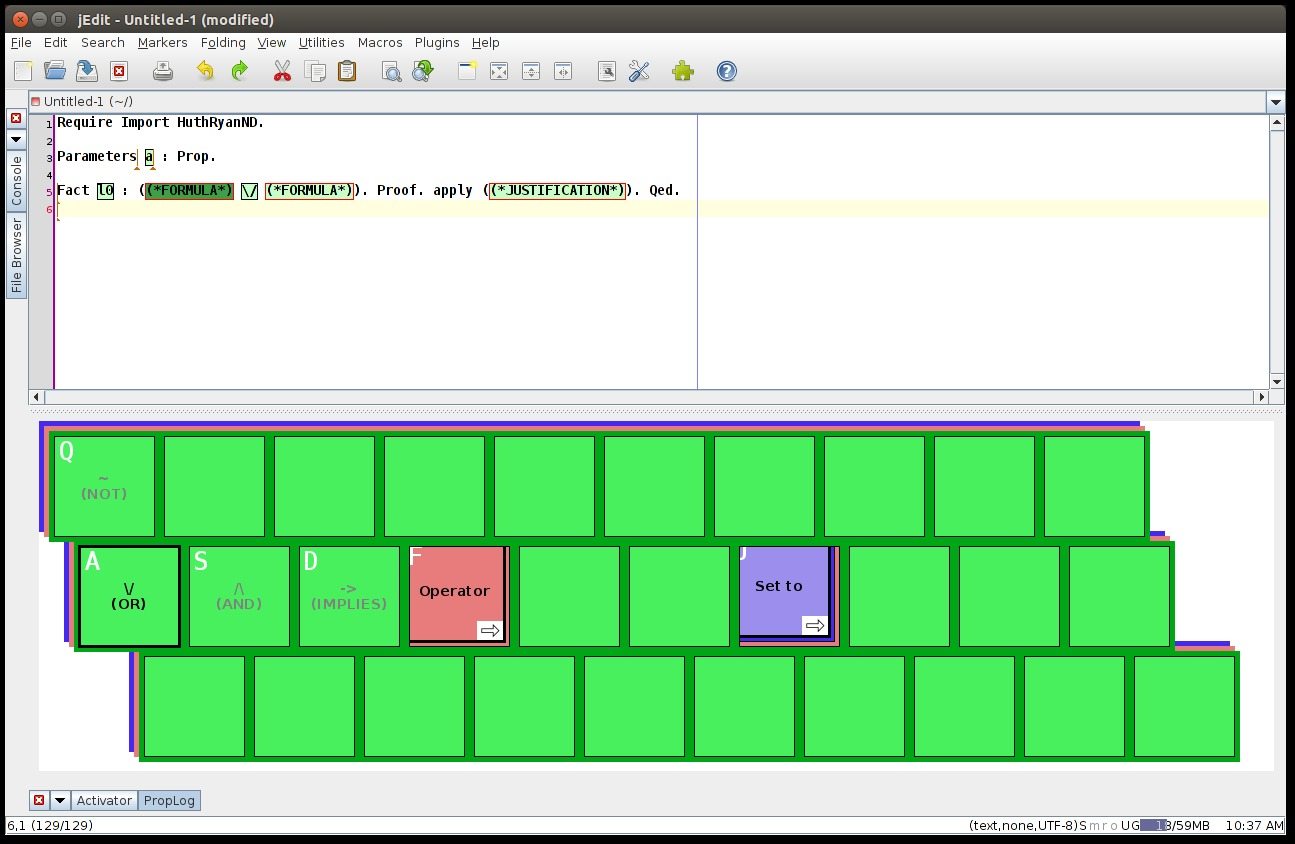
\includegraphics[width=\linewidth]{pl6.jpg}
  \caption{}
  \label{fig:pl6}
\end{figure}

Without having to lift one's index fingers, one can then replace the first of the two new formula placeholders with another binary operator and pair of placeholders.  Not shown, one could have used the ``Add to right'' submenu to replace the current formula, call it ``A'', with a binary operator whose left subformula is A and whose right subformula is selected.  

\begin{figure}[H]
  \center
  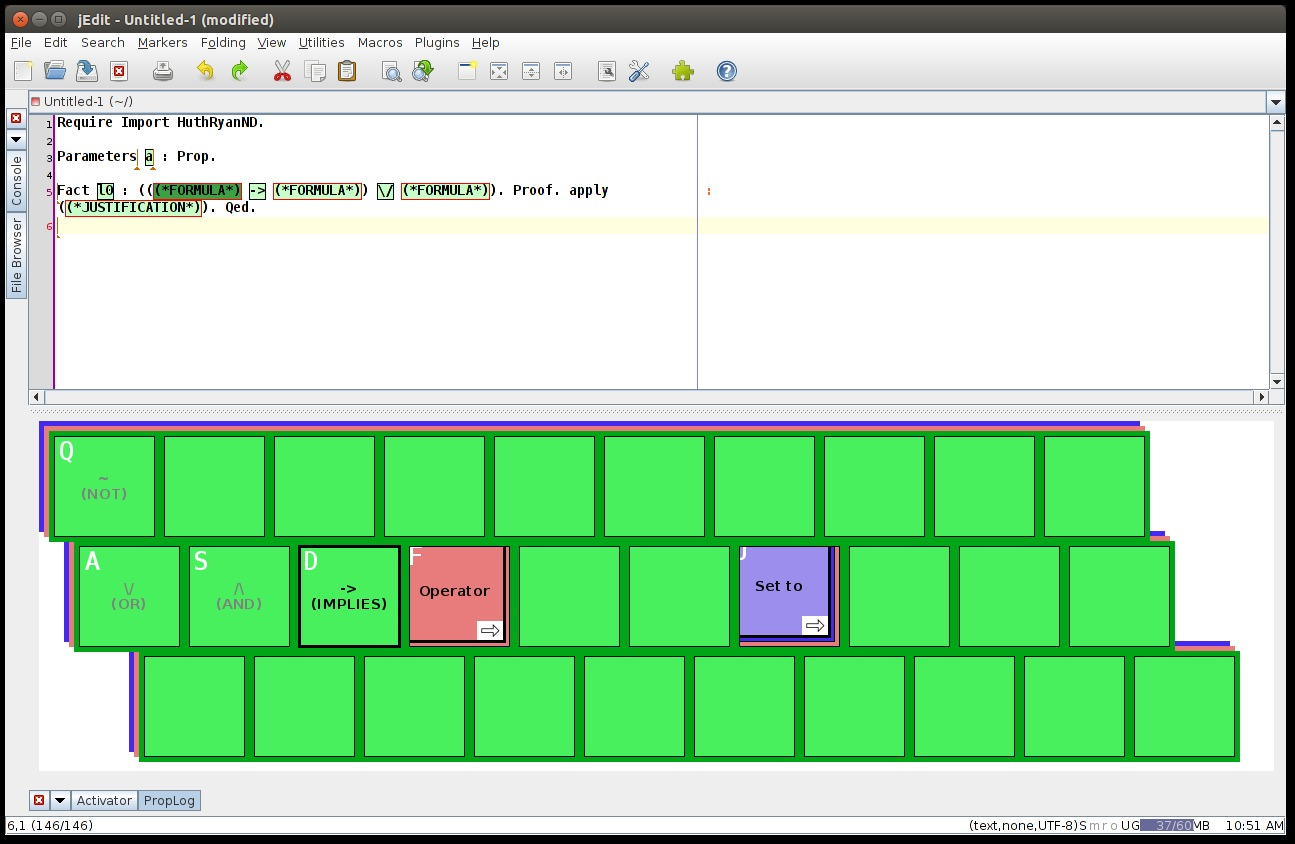
\includegraphics[width=\linewidth]{pl7.jpg}
  \caption{}
  \label{fig:pl07}
\end{figure}

There are actually two different selection modes.  Leaf mode, which we have seen, draws green highlights over selectable leaves and the user can move left and right among these.  Branch mode, seen in \autoref{fig:pl8}, draws brown highlights over a set of sibling nodes.

\begin{figure}[H]
  \center
  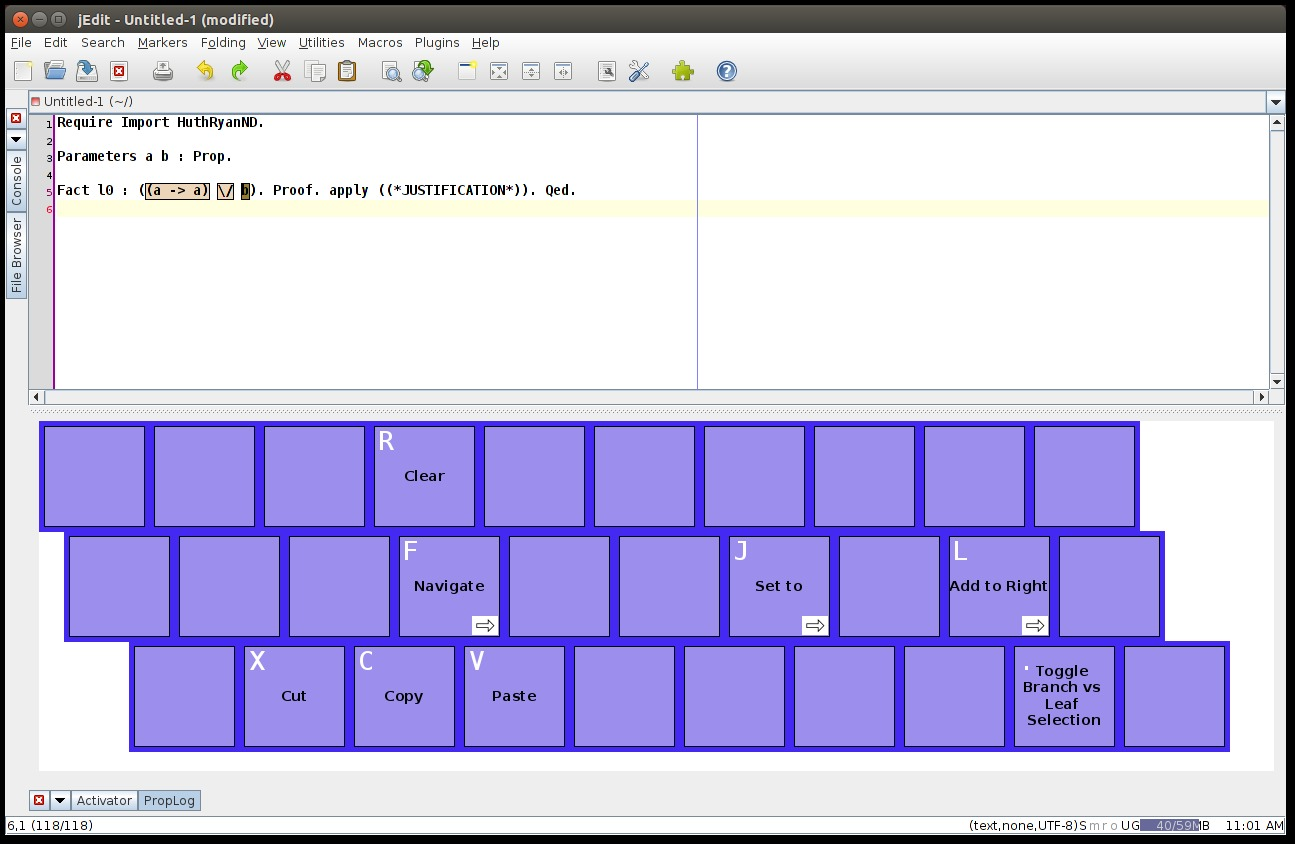
\includegraphics[width=\linewidth]{pl8.jpg}
  \caption{}
  \label{fig:pl8}
\end{figure}

Users can move left, as seen in \autoref{fig:pl9}...

\begin{figure}[H]
  \center
  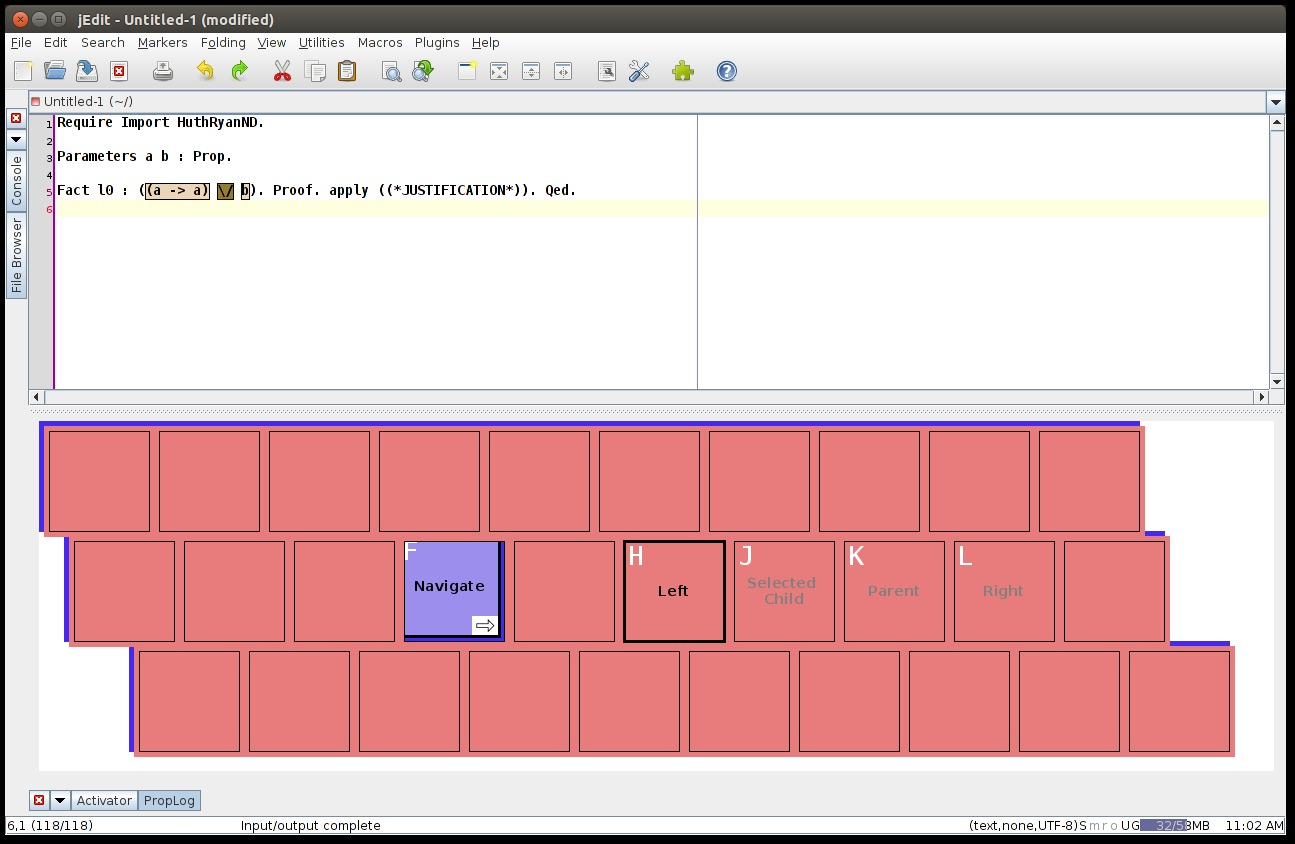
\includegraphics[width=\linewidth]{pl9.jpg}
  \caption{}
  \label{fig:pl9}
\end{figure}

...to the parent, as seen in \autoref{fig:pl10}...

\begin{figure}[H]
  \center
  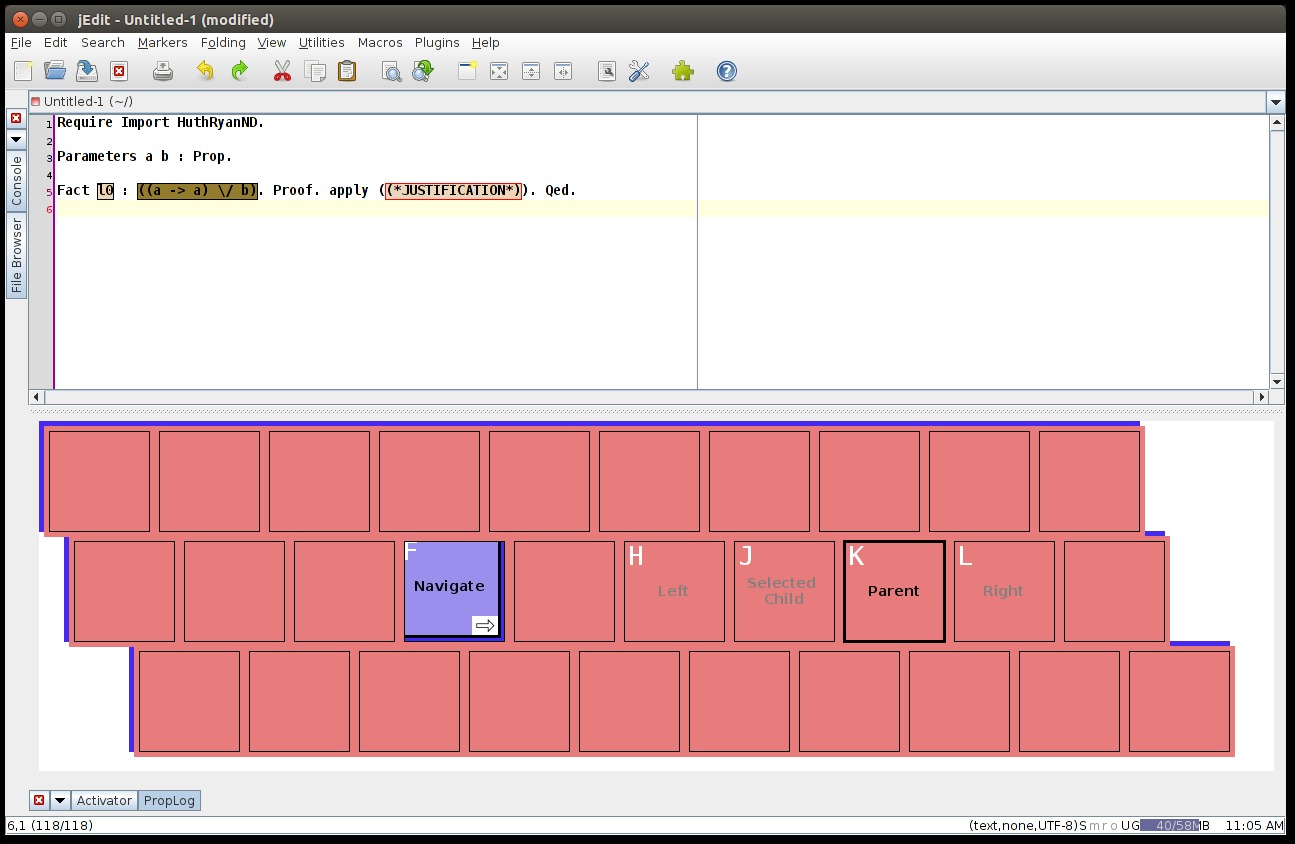
\includegraphics[width=\linewidth]{pl10.jpg}
  \caption{}
  \label{fig:pl10}
\end{figure}

...right, as seen in \autoref{fig:pl11}...

\begin{figure}[H]
  \center
  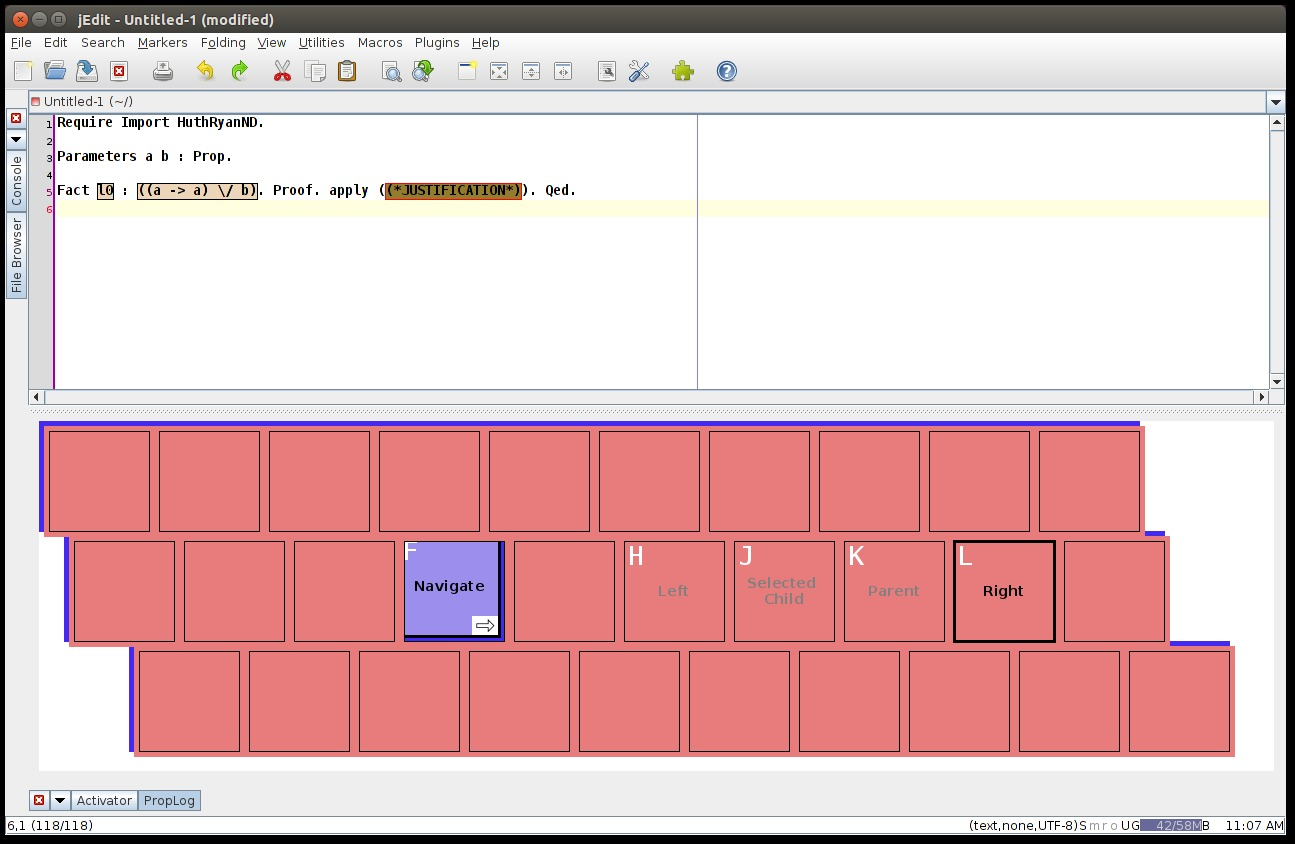
\includegraphics[width=\linewidth]{pl11.jpg}
  \caption{}
  \label{fig:pl11}
\end{figure}

...or back to the selected child node.  Other selection modes (e.g. movement using in-order or level order traversal) may be considered in future iterations of the design process.

%=============================================================================
\chapter{Related Work}
\label{chapter:relatedwork}
%=============================================================================

The need for effective theorem prover user interfaces has been recognized for over 20 years (e.g. \cite{Thery:1992:RTP:142868.143760}) and a series of conferences has even been organized to address this need specifically.\footnote{See http://www.informatik.uni-bremen.de/uitp/ for more information} Many interesting and helpful ideas have been proposed, both for Coq and for related systems.  These ideas vary widely and include integration of Coq, and other theorem provers, with dynamic geometry software \cite{narboux2007graphical,quaresma2007geothms}, easier-to-read declarative languages for proof scripts \cite{corbineau2008declarative}, using wikis for creating proof repositories \cite{corbineau2007cooperative}, and automating the process of using libraries \cite{asperti2010some}.

One approach taken to improve theorem prover user interfaces has been ``Proof by Pointing''\cite{bertot1994proof}, an algorithm to build a proof tree by pointing to portions of a goal.  This was implemented in the \textit{CtCoq} interface \cite{bertot1996ctcoq}, again, later, in the Java-based Pcoq interface \cite{amerkad2001mathematics} and also in the \textit{Jape} system \cite{bornat1999animating}.  Note that some schemes for writing and displaying proofs, notably Fitch style proofs, do not display hypotheses with their conclusion, which may lead to ambiguity when using Proof by Pointing \cite{bornat1997displaying}. 

An example of a recent project is \textit{Panoptes} \cite{farmer2009panoptes}, which allows visualization of proofs produced by the IMPS Interactive Mathematical Proof System.  The system has numerous features allowing users to zoom in on parts of the graph, collapse nodes, rearrange the positions of nodes, label and highlight nodes, and inspect details associated with nodes using pop-up windows.  While these features allow the user to manipulate the presentation of a proof, they do not allow the user to manipulate the proof itself---to change the proof, one must use an Emacs-based environment.

Another significant project is an interactive visualizer for the \textit{ACL2} theorem prover\cite{ACL2}, described in \cite{bajaj2003interactive}.  This tool allows for visualization at three different levels.  It does so first at the level of relationships between theorems and their proofs (the directed acyclic graph describing which lemmas from which libraries are used to prove a given theorem).  Next, it shows a proof tree
%, similar to the visualization given in section \ref{prooftransitions}, 
where a node represents a statement that is being proved using the node's children.  Color coding is used here to indicate the action taken by the prover at a node, and the tree is represented using three-dimensional ``cone trees.''  The contents of the individual nodes, as text, can also be displayed alongside this tree.  At the third level, this text's syntax tree can be visualized (as lines connecting points again, though in a more usual two-dimensional arrangement, and still in contrast with the Syntax Tree Highlighting discussed above).  Selecting text at this level will highlight the corresponding portion of the tree visualization.  The system also supports textual pattern matching, where the degree of matching is indicated by the color of the text and the tree visualization.  Both at this level and at the proof structure level (i.e. the second level) the system is capable of zooming and panning, and, at the proof structure level, rotating is also possible.

A few other significant projects aiming to improve the presentation of machine-checked proofs include \textit{Proviola}, which allows users to move through a proof script displayed on a web page and view the results that Coq would produce \cite{tankink2012narrating}; an ``Interactive Derivation Viewer'' for visualizing derivations written in the TPTP language \cite{trac2007interactive}; the LOUI interface for the OMEGA proof assistant, featuring graphical visualization, term browsing, and natural language proof presentation \cite{siekmann1999loui}; and the Tecton system, featuring tree visualization combined with hypertext navigation of nodes \cite{kapur1994overview}.  Theoretical and methodological work has also been done and can be seen in \cite{eastaughffe1998support,bertot1998generic,luth1999functional,volker2004thoughts,geuvers2009proof}, and \cite{luth2009user}.  Work aimed at making ITPs more suitable for novices and educational settings includes \cite{tsovaltzi2003approach,meier2004adaptable,narboux2007graphical,billingsley2007student,dillinger2007acl2s,hendriks2010teaching,schreiner2009risc} and \cite{pierce2010proofassist}.

In addition to previous work specifically on theorem prover user interfaces, it is important to consider more general human-computer interaction research and research on software development tools.  Starting with the latter, one can consider the data of \cite{murphy2006java} showing that the Eclipse IDE's ``rename,'' ``move,'' ``extract'', and ``inline'' refactoring commands are in fact used by many programmers and are frequently invoked via key bindings.  The data also shows that a large percentage of \textit{all} commands executed by developers using the IDE extensively were invoked via key bindings, and one of the top commands was ``content assist'', which suggests possible text to insert (similar to Proof Previews, though it does not show the effects of evaluating this text).  One may also note, here, the existence of various lines of work, e.g. the \textit{Frama-C} \cite{FramaC} project, aimed at integrating theorem proving and programming within IDEs, and the \textit{KeY} \cite{beckert2007verification} project (for ``Integrated Deductive Software Design'') which integrates graph visualization with theorem proving in the Eclipse IDE.

In addition to IDEs, we may consider software visualization tools:  \cite{bassil2001software} reports on a survey of users of software visualization tools such as \textit{daVinci} (now called \textit{uDraw(Graph)}), \textit{GraphViz}, \textit{Grasp} (now \textit{jGrasp}), and \textit{Tom Sawyer Software}--more than 40 different tools altogether.  Some of the ``functional aspects'' of the software visualization tools that were considered most useful, and that might also have useful analogs in theorem prover user interfaces, were ``search tools for graphical and/or textual elements'', ``hierarchical representations'' and ``navigation across hierarchies'', ``use of colors'', and ``easy access, from the symbol list, to the corresponding source code.''  Among functional aspects considered least useful were ``3D representations and layouts, and virtual reality techniques'' and ``animation effects'', though the later was considered ``quite useful'' when the software was implemented in a declarative language.  Software visualization tools were considered beneficial in increasing productivity and managing complexity, and were considered particularly important in the ``software comprehension process.''

A survey and taxonomy of software visualization is presented in \cite{caserta2011visualization}.  Similar to \cite{bajaj2003interactive}, it divides tools into three groups according to their use at three different levels of abstraction: line, class, and architecture.  They also differentiate between tools used for visualizing code at a particular time and those that allow for visualization of the evolution of software.  Many of the techniques used by these tools could be applied to visualization for interactive theorem provers.  \textit{Seesoft} \cite{eick1992seesoft}, for instance, miniaturizes lines of code with lines of color-coded pixels, and \textit{sv3D} \cite{marcus20033d} extends this idea using three-dimensional arrays of blocks where information about lines of code is encoded in the height and color of the blocks.  Other techniques potentially useful for interactive theorem prover user interfaces include using animation and color gradients to show the direction of relationships between software components \cite{alam2007evospaces,holten2006hierarchical} and using texture and 3D object primitives called ``geons'' to encode additional information \cite{holten2005visual,irani2001using}.

The more general human-computer interaction literature on tree visualization is quite extensive--many techniques have been developed.  Four different ``common layouts'' are listed in \cite{holten2006hierarchical}: rooted tree
%(the node layout presented, for instance, in \autoref{fig:similarnodes}, with 
(child nodes arranged on a horizontal line above or below their parents), radial trees (nodes of each level of the tree are arranged in concentric circles, with the root node at the center, its children at the first circle out, their children at the next circle out, etc.), balloon trees (each parent's child nodes are arranged radially around the parent), and treemaps (which divide a rectangle into smaller and smaller rectangles with the largest rectangle representing the root of the tree and the smallest representing the leaves, and where division of the rectangles switches between using horizontal and vertical lines when going between tree levels; these were developed in \cite{shneiderman1992tree}).  These common layouts have been extended in various ways.  For instance, \cite{nguyen2002space} describes a space-optimized version of balloon trees and \cite{van1999cushion} describes the the addition of gradients to the rectangles in treemap visualizations, making the structure of the tree easier to see.

\cite{katifori2007ontology} presents an extensive review of tree visualization techniques.  Along with classifying visualizations as 2D or 3D (or 2.5D when no movement in or manipulation of a 3D visualization is allowed), it divides the visualizations into six overlapping categories: indented list, node-link and tree, zoomable, space-filling, focus+context or distortion, and three-dimensional information landscapes.  Indented lists can be seen in file system browsers, e.g. \textit{Microsoft Windows}' \textit{Explorer}, the rooted and radial trees mentioned in \cite{holten2006hierarchical} as common layouts are ``node-line and tree'' type, and treemaps are an example of the space-filling type.  An example of a zoomable visualization is \textit{Grokker} \cite{rivadeneira2003study} which allows users to click and expand nested circles.  An example of the focus+context or distortion category is the \textit{Hyperbolic Browser} \cite{lamping1996hyperbolic} which magnifies and centers on the area around a selected node in a radial layout.  An example of a three-dimensional information landscape is the \textit{Harmony Information Landscape} \cite{eyl1995harmony}.


%=============================================================================
\chapter{Summary and Conclusions}
%=============================================================================

This document contributes in several ways.  First and foremost are the development of user interface prototypes and their evaluation.  These prototypes include novel applications and implementations of existing user interface ideas to interactive theorem proving: the automatic reorganization of the layout of the tree visualizatio used in Proof Transitions, representation of the cached evaluated section in the basic CoqEdit environment, the presentation of suggestions in Proof Previews.  The prototypes also include new schemes for interacting with proofs that may be generalized to work with many other software applications:  keyboard-card menus, syntax tree highlighting, and text-manipulation visualization seen in Proof Transitions.

In addition to these user interface ideas, insight into several other issues is provided.  One lesson learned in testing Proof Transitions is that the Paradox of the Active User--that users may be too busy using software to explore its features--may extend further than one might expect:  not only do inexperienced computer users fail to take advantage of shortcuts when dropdown menus are available, but experienced computer science students often also fail to take advantage of keyboard commands even when interaction using the mouse is not available.  This is evidence of the importance of the design principle that one should make taking advantage of features unavoidable (at least by default).

Another lesson learned is on how user interface studies for interactive theorem provers may be conducted.  The original plan for evaluating the effectiveness of Proof Transitions was to do a blind grading of proof explanations using 
Unfortunately, it turned out (in the pilot testing for the experiment) that the explanations given by participants would make no sense without an accompanying view of the screen (so blind grading became impossible).\footnote{The natural way of explaining the proofs turned out to be to explain what each tactic did as one moved through the proof, rather than describing the overall structure and important points in the proof as we had expected.  This was probably the result of limiting the number of tactics to which participants were exposed (and only using propositional logic) while still keeping the proofs complex by having many branches.}  The solution to evaluating the effectiveness of Proof Transitions turned out to be looking for more objective ways in which Proof Transitions might be better.  One attempt at doing this was by encouraging participants to give specific information about the effects of each tactic (e.g. how many nodes does it produce); participants largely seemed to find either that these instructions were confusing or that such precise detail about each node was unimportant for their explanations of the proofs (which was probably reasonable, since many tactics produced similar or identical results).  The solution that ultimately worked, looking at whether participants stated when a destruct tactic created two child nodes, involved looking at what participants actually included in their proof explanations (rather than what we expected would be in them) and did not require forcing participants to change their behavior.

The final contribution to be mentioned is simply the set of results obtained.  With Keyboard-Card Menus, we have evidence that users are capable of interacting with a computer through a new interface and that the presentation used by this interface has learnability advantages over dropdown menus.  With the Proof Previews experiment results, we have evidence that the menu of suggestions allow users to complete more proofs in less time, and that users usually prefer using the feature to typing out the proof character by character.  

With Proof Transitions, although a majority of participants did not prefer the new interface, one must bear several facts in mind.  First, this was not a winner-take-all comparison and a large minority of participants did in fact prefer the Proof Transitions interface; one-size-fits-all is probably not what is needed in theorem prover user interfaces, and, as suggested by both the novice users in the study and experienced users in the earlier survey, many-sizes-to-fit-each may be more appropriate (e.g. a user interface for teaching or presenting proofs vs. a user interface for writing them).  Second, this large minority was present despite the experiment being biased against Proof Transitions (since the prototype version of Proof Transitions that was presented to participants did not allow proofs to be written or edited, though a non-prototype version might, and since the tutorial that was seen by participants was presented primarily using the basic interface).  Third, there are many ways in which Proof Transitions could be refined to boost user preference for it higher, as discussed below.

This brings us to the question of where to go from here.  I see at least four major paths.  First is the next iteration of \textbf{refinement and testing of Proof Transitions}.  This might include:

\begin{itemize}
 \item Automatically adding visit-marks (the purple squares seen in \autoref{fig:ptvisitednode}) to nodes as they are visited.  The original rationale for not doing so was that users would want to only mark nodes they had actually taken a close look at and felt comfortable they understood (which, as far as I can tell, is still accurate), and it is very easy to navigate through the tree without actually looking at the contents of the nodes.  The problem was that users forgot to use the visit-mark feature.  Reasonable compromises might be 1) to add the marks only after the user had continuously been at the node, zoomed in, for a few seconds) to gradually make the mark fade in as the user remained at the node.
 \item Improvements to the transition highlighting and animation (i.e. blinking yellow highlighting).  Making the animation play automatically when one moves to a node would be one improvement, since users tended to forget about the animation's existence.  Giving the user the ability to move through the matching text at his own pace (e.g. by pressing keys) might be another; one could then allow the animation to be played more quickly when one moves to the node, knowing that the user has the opportunity to go back at a slower pace.  It also seems unlikely that blinking highlighting is the best way to match sections of text; other options that may be more salient include drawing lines between matching locations and making a copy of the text float to its matching location.
 \item One major advantage of the basic CoqEdit interface seems to be the fact that node traversal was linearized--the user is forced to go through the nodes in a particular order.  This means faster traversal of the proof tree, as well as making it easy to tell which nodes have been visited. Adding forwards and backwards commands for both in-order and level-order would be relatively straightforward (though it might be helpful to zoom out during the larger jumps).
 \item Having a mini-map, rather than forcing users to go through the extra step of zooming out, might make it easier to keep track of where one is within the tree.  At the same time, one could allow for more than two zoom levels so that users could inspect branches of the proof tree (as well as pairs of nodes or the entire tree structure).
\end{itemize}

There are also some longer-term issues to be addressed.  Perhaps the most challenging would be a mechanism for getting sets of matching text resulting from tactic use on particular goals.  While it may be best to leave to back-end developers the task of providing commands to print out relevent information\footnote{This would be analogous to a command line debugging tool for a programming language.}, there are also probably still more design decisions regarding what that information includes as well has how to present it to the user.  For example, a user might be interested in the procedure by which a tactic is executing other tactics (e.g. the fact that the ``intros'' tactic repeatedly executes the ``intro'' tactic).

Other longer-term work on Proof Transitions includes:

\begin{itemize}
 \item Integrating the visualization with the editing environment.  Presumably this will follow a model similar to that of Proof Web (see \autoref{fig:proofweb}), but inevitably there will be some complications.  One important difference with Proof Web that I hope to see is the ability to edit the proof script ``from the visualization'' at arbitrary nodes in the proof tree; this would require some automatic code generation and, ideally, automatic code formatting.
 \item Dealing with nodes containing large amounts of text.  One solution here would be to make the nodes scrollable (like ordinary windows).  Other solutions that might work better with the text matching visualization might be to shrink the node's text or to expand the box containing the text.  Hybrid solutions are another possibility.
 \item Visualizing advanced tactics that actually have effects on unproved goals other than the current goal.  These tactics are not necessary, and users could be prevented from using these, but some relatively minor modifications to the existing visualization could probably be used to represent these.
\end{itemize}

A second path for future research would be to \textbf{fully implement Proof Previews}.  One complicating aspect of this is performance:  how to index libraries, and perhaps use some parallel processing, to generate a list of possible tactics and theorems to apply in real time.  Two additional related problems are how to put the most helpful suggestions at the top of the list and how to avoid not only tactics that immediately produce errors, but also tactics that produce unprovable subgoals.  This could be very challenging as it involves techniques from automated theorem proving (a discipline in its own right).

A third path would be to \textbf{improve and optimize Keyboard-Card Menus, Syntax Tree Highlighting, and their combined use}.  \autoref{section:kcm} discusses many possible avenues for future work on Keyboard-Card Menus.  Two more, not mentioned there, would be 1) to explore different sets of keys (e.g. consider keyboard-cards that include the SHIFT keys), and 2) to experiment with providing more detailed information about the effects of invoking a command (e.g. pressing and holding a key for several seconds might be equivalent to hovering over an icon with the mouse instead of clicking it).  Other areas to work on include:

\begin{itemize}
% \item commands for larger templates
 \item Providing alternative ways to traverse the syntax tree, e.g. if one runs out of siblings when moving the right, does moving to an uncle on the right feel seem natural?
 \item Optimizing the set of commands and their placement in the keyboard-card hierarchies.
 \item Working with other languages, e.g. 1st order logic, programming languages, or Coq's full ``vernacular'' language---part of the rationale for developing Syntax Tree Highlighting was to make clear how to parse expressions in Coq that often involve deep nesting of subexpressions and non-standard or user-defined notations/precedences. 
\end{itemize}

A fourth and final path would be to step back and \textbf{re-evaluate the design of traditional text editors}.  One can think of the Proof Transitions as a non-traditional editor (the prototype being only available for read-only documents).  Given larger amounts of screen space, keyboard-card menus and other new input techniques, and programming interfaces for zoomable user interfaces, work in this direction seems appropriate.

%I hope that this document will inspire further research along one or more of these paths.


%=============================================================================
% \appendix
% %=============================================================================
% 
% %=============================================================================
% \chapter{Sample Appendix}
% 
% \section{Appendix One}
% \blindtext
% 
% \section{Appendix Two}
% \blindtext
% 
% %=============================================================================
% \chapter{Another Appendix}
% 
% \section{Appendix Three}
% \blindtext
% 

%=============================================================================
% bibliography
%=============================================================================
\interlinepenalty=10000	% prevents bib items from splitting across pages
\bibliographystyle{uithesis}
\bibliography{thesis}

\end{document}
